% This LaTeX document needs to be compiled with XeLaTeX.
\documentclass[a4paper]{article}
%\documentclass[10pt]{article}
\usepackage[utf8]{inputenc}
\usepackage{graphicx}
\usepackage[export]{adjustbox}
\graphicspath{{./images/}{../cose da aggiungere/pittogrammi/}{../cose da aggiungere/privacy_conformita/}}
\usepackage{caption}
\usepackage{amsmath}
\usepackage{amsfonts}
\usepackage{amssymb}
\usepackage[version=4]{mhchem}
\usepackage{stmaryrd}
\usepackage{multirow}
\usepackage{hyperref}
\hypersetup{colorlinks=true, linkcolor=blue, filecolor=magenta, urlcolor=cyan,}
\urlstyle{same}

\usepackage{float}
\usepackage{tabularx}
\usepackage{array}

\usepackage{titling}
\pretitle{\begin{center}
\includegraphics[width=\textwidth]{../cose da aggiungere/header_WATT+}\\[6em]}
	\posttitle{\end{center}}

\usepackage[fallback]{xeCJK}
\usepackage{polyglossia}
\usepackage{fontspec}
\usepackage{newunicodechar}
%\IfFontExistsTF{Noto Serif CJK JP}
%{\setCJKmainfont{Noto Serif CJK JP}}
%{\IfFontExistsTF{STSong}
%  {\setCJKmainfont{STSong}}
%  {\IfFontExistsTF{Droid Sans Fallback}
%    {\setCJKmainfont{Droid Sans Fallback}}
%    {\setCJKmainfont{SimSun}}
%}}

\setmainlanguage{italian}
\IfFontExistsTF{CMU Serif}
%{\setmainfont{CMU Serif}}
%{\IfFontExistsTF{DejaVu Sans}
%  {\setmainfont{DejaVu Sans}}
%  {\setmainfont{Georgia}}
%}

%New command to display footnote whose markers will always be hidden
\let\svthefootnote\thefootnote
\newcommand\blfootnotetext[1]{%
  \let\thefootnote\relax\footnote{#1}%
  \addtocounter{footnote}{-1}%
  \let\thefootnote\svthefootnote%
}

%Overriding the \footnotetext command to hide the marker if its value is `0`
\let\svfootnotetext\footnotetext
\renewcommand\footnotetext[2][?]{%
  \if\relax#1\relax%
    \ifnum\value{footnote}=0\blfootnotetext{#2}\else\svfootnotetext{#2}\fi%
  \else%
    \if?#1\ifnum\value{footnote}=0\blfootnotetext{#2}\else\svfootnotetext{#2}\fi%
    \else\svfootnotetext[#1]{#2}\fi%
  \fi
}

\newunicodechar{□}{\ifmmode\square\else{$\square$}\fi}
\newunicodechar{✓}{\ifmmode\checkmark\else{$\checkmark$}\fi}

\title{\Huge{SKIN ANALYZER+}}
\date{}

\begin{document}
	
\maketitle

%\section{MANUALE D'USO Skin Analyzer+}

\begin{figure}[H]
	\centering
	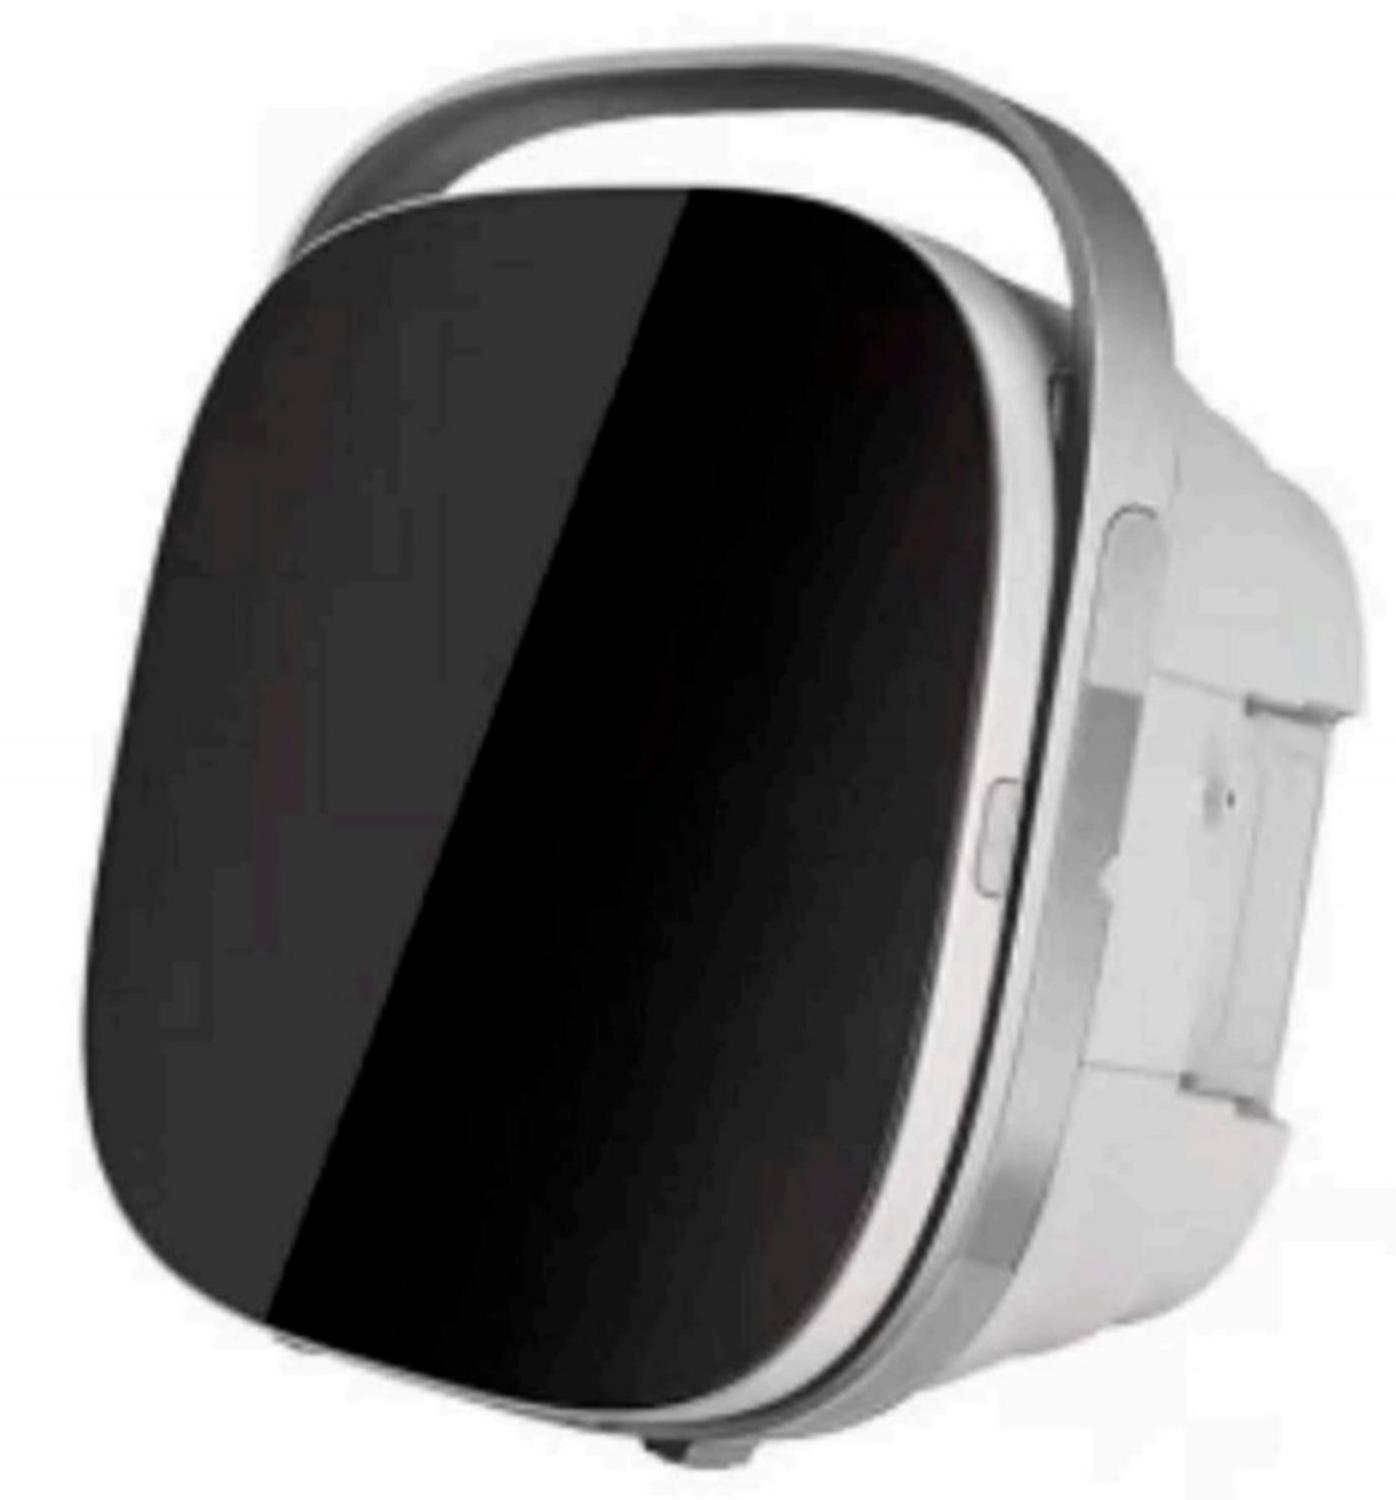
\includegraphics[width=0.6\textwidth]{018f02f8-3740-46eb-ab06-ecd68977d8ca-01_1500_1396_974_2415}
	\captionsetup{labelformat=empty}
%	\caption{Si prega di leggere attentamente questo manuale prima di installare e utilizzare l'strumento.}
\end{figure}

\newpage
Si prega di leggere attentamente questo manuale prima di installare e utilizzare lo strumento.

\section*{Dichiarazione}
Grazie per aver acquistato il sistema di analisi della pelle.\\
Si prega di leggere attentamente questo manuale prima di installare e utilizzare il dispositivo.

Vengono apportate modifiche senza preavviso a causa di aggiornamenti e miglioramenti del prodotto.

Dichiarazione: I diritti d'autore del manuale utente appartengono al produttore originale e il suo contenuto non può essere copiato o diffuso senza autorizzazione scritta.

L'azienda si impegna a garantire che le informazioni contenute in questo manuale siano accurate e affidabili. Tuttavia, non fornisce alcuna forma di garanzia, inclusa, ma non limitata a, la garanzia implicita di idoneità commerciale e idoneità per un particolare scopo. L' azienda non sarà ritenuta responsabile di alcuna perdita o danno, compresi i risultati dell'utilizzo di queste informazioni o i danni speciali causati, anche qualora tale perdita o danno derivi da negligenza o da altri errori commessi dall'azienda.

\newpage

\tableofcontents

\newpage

\section{Simboli}
\begin{figure}[H]
	\centering
	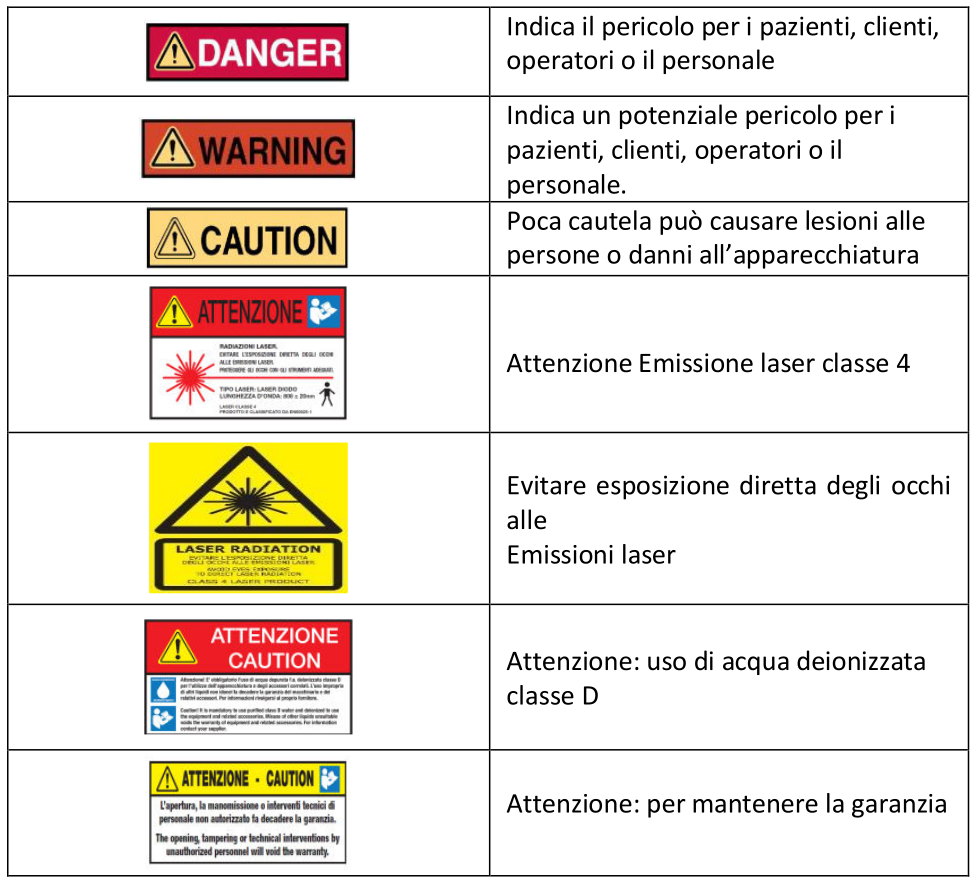
\includegraphics[width=\linewidth]{pittogrammi_1}
%	\caption{}
	\label{fig:pittogrammi1}
\end{figure}
\begin{figure}[H]
	\centering
	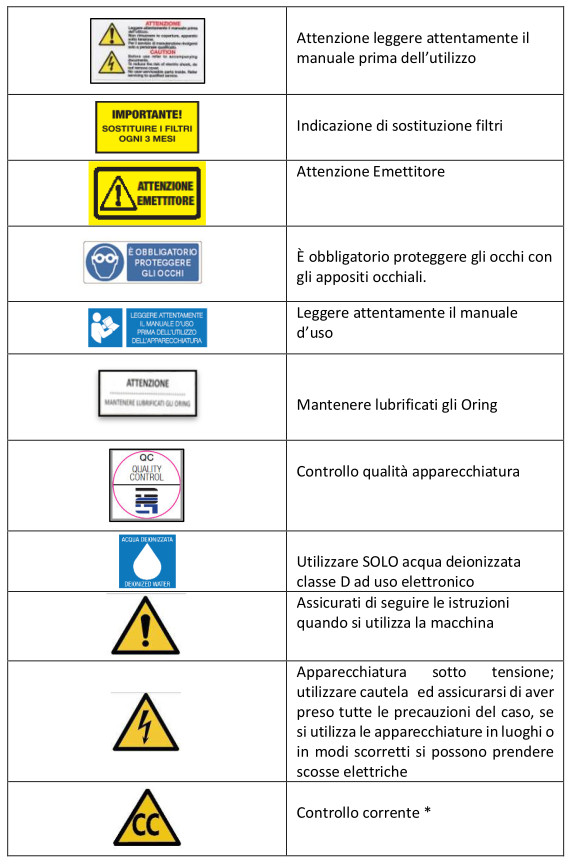
\includegraphics[width=\linewidth]{pittogrammi_2}
%	\caption{}
	\label{fig:pittogrammi2}
\end{figure}
\begin{figure}[H]
	\centering
	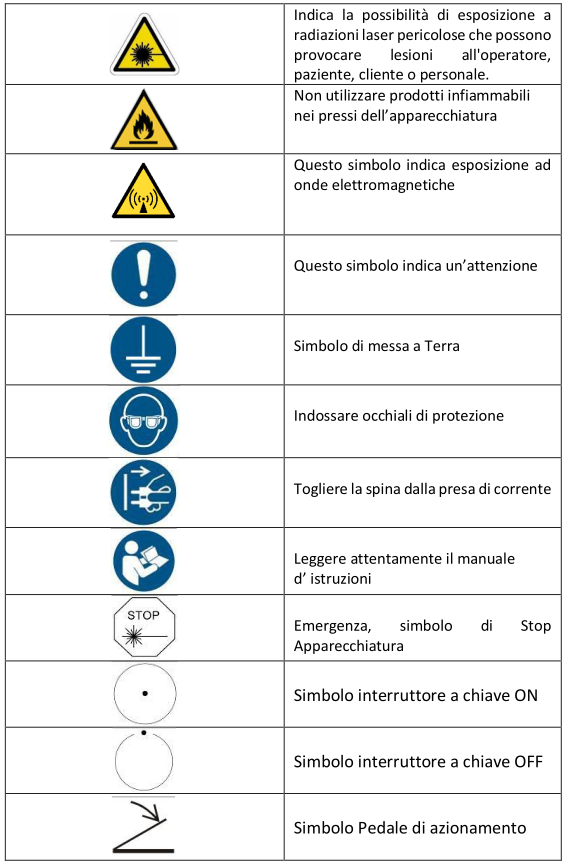
\includegraphics[width=\linewidth]{pittogrammi_3}
%	\caption{}
	\label{fig:pittogrammi3}
\end{figure}
\begin{figure}[H]
	\centering
	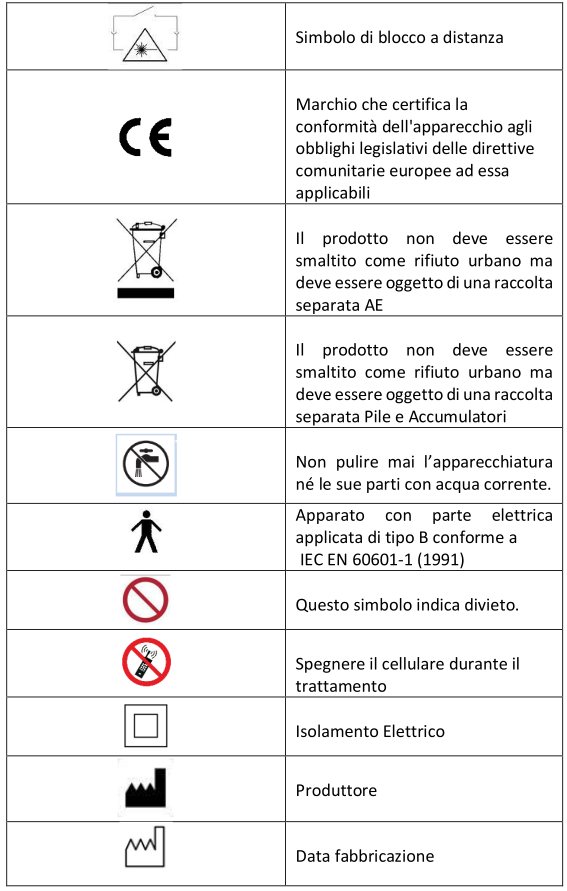
\includegraphics[width=\linewidth]{pittogrammi_4}
%	\caption{}
	\label{fig:pittogrammi4}
\end{figure}
\begin{figure}[H]
	\centering
	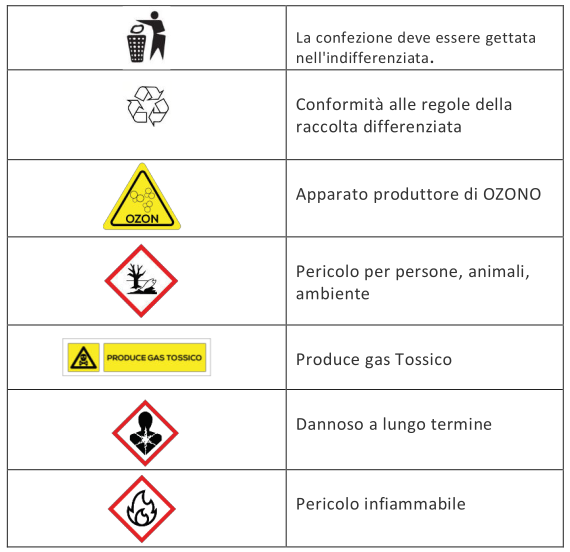
\includegraphics[width=\linewidth]{pittogrammi_5}
%	\caption{}
	\label{fig:pittogrammi5}
\end{figure}


\newpage

\section{Struttura e accessori}
\begin{center}
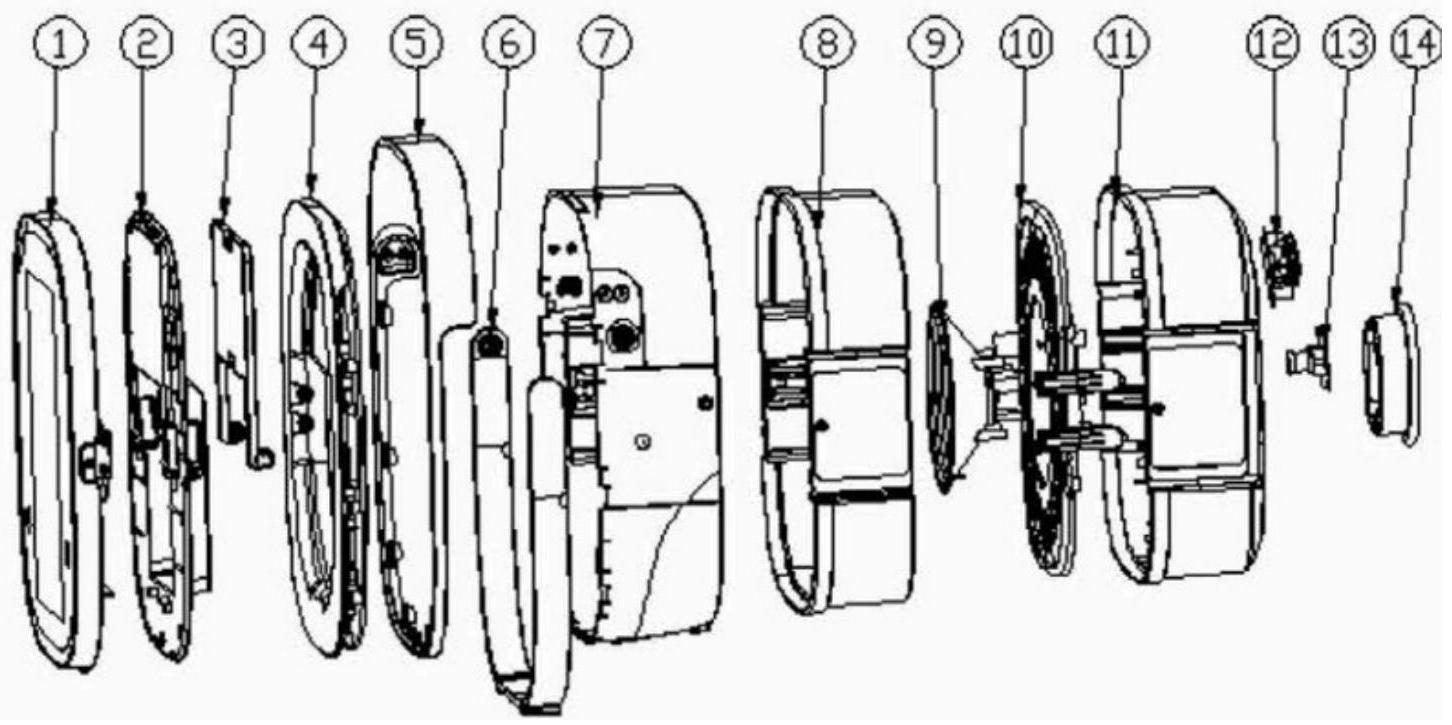
\includegraphics[max width=\textwidth, alt={}]{018f02f8-3740-46eb-ab06-ecd68977d8ca-04_725_1452_432_213}
\end{center}

\begin{center}
\begin{tabular}{|l|l|l|l|}
\hline
N0. & Nome & QTY & NOTA \\
\hline
1 & Mostra la copertina anteriore & 1 &  \\
\hline
2 & Visualizza la copertina posteriore & 1 &  \\
\hline
3 & Supporto per lo schermo & 1 &  \\
\hline
4 & Cassetta anteriore del corpo principale & 1 &  \\
\hline
5 & Handle & 1 &  \\
\hline
6 & Sostegno del corpo principale & 1 &  \\
\hline
7 & Copertina anteriore del corpo principale & 1 &  \\
\hline
8 & Coperchio centrale del corpo principale & 1 &  \\
\hline
9 & Armadio per fotocamere & 1 &  \\
\hline
10 & Pannello luminoso a LED & 1 &  \\
\hline
11 & Rivestimento posteriore del corpo principale & 1 &  \\
\hline
12 & Pannello di controllo & 1 &  \\
\hline
13 & Accessori per pulsanti & 1 &  \\
\hline
14 & Copertura accessoria & 1 &  \\
\hline
\end{tabular}
\end{center}

\section{Parametri}
\begin{itemize}
	\item Potenza: 20 W
	\item Tensione dell'adattatore: 110-230 VAC $\pm 10 \%$; tensione del corpo principale o pannello: $12 \mathrm{~V} \mathrm{CC} / 3 \mathrm{~A}$
	\item Piattaforma operativa: Android 8.1
	\item Camera: fotocamera HD da 20 milioni di pixel
	\item Modalità fotografia: Modalità automatica
	\item Dimensione dello schermo: 10,1 pollici
	\item Memoria in esecuzione: 2 GB
	\item Spazio di archiviazione: 64 GB
	\item Estensione esterna: supporto per schede SD esterne
	\item Connessione tra host e tablet: Wi-Fi/USB Luce specchio: tre colori di luce regolabili
	\item Dimensioni della macchina: $34 \mathrm{~cm} \times 30 \mathrm{~cm} \times 12 \mathrm{~cm}$
	\item Pacchetto Dimensioni: $43 \mathrm{~cm} \times 22 \mathrm{~cm} \times 41 \mathrm{~cm}$
	\item NW:3.5KG
	\item GW:4.8KG
\end{itemize}

\section{Installazione}
\subsection{Installazione}
\begin{enumerate}
  \item Il cavo di alimentazione e il cavo dati del tablet sono collegati rispettivamente al computer e al tablet; in questo momento l'indicatore verde è acceso, come
\end{enumerate}

\begin{figure}[H]
\begin{center}
  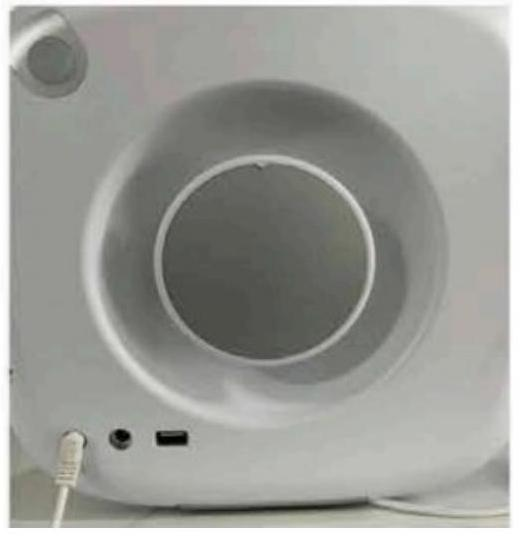
\includegraphics[alt={},max width=\textwidth]{018f02f8-3740-46eb-ab06-ecd68977d8ca-05_538_521_697_297}
\captionsetup{labelformat=empty}
\caption{Immagine 3-1}
\end{center}
\end{figure}

mostrato nella figura 3-13-2.

\begin{figure}[H]
\begin{center}
  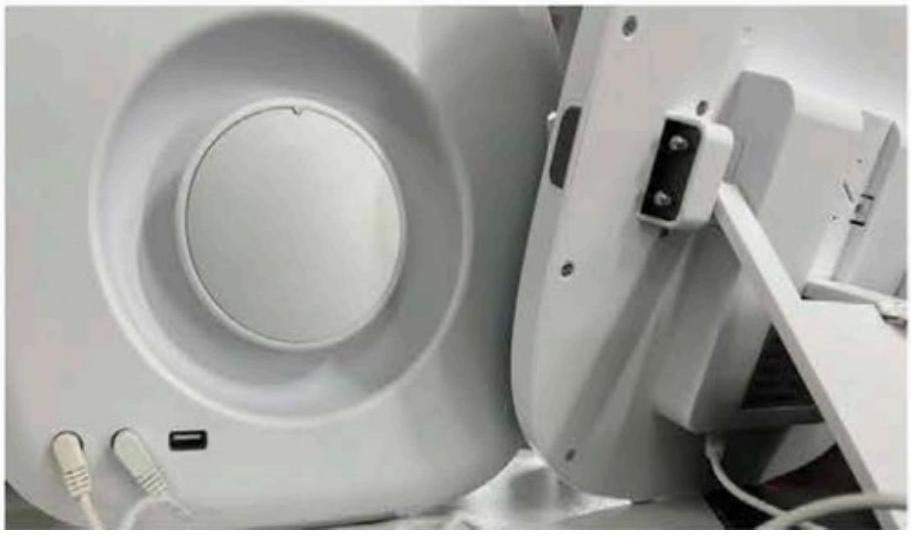
\includegraphics[alt={},max width=\textwidth]{018f02f8-3740-46eb-ab06-ecd68977d8ca-05_538_915_697_872}
\captionsetup{labelformat=empty}
\caption{Immagine 3-2}
\end{center}
\end{figure}

\begin{enumerate}
  \setcounter{enumi}{1}
  \item Aprire il supporto per la pastiglia e fissare i due supporti nella scanalatura per fissarla, come mostrato nella figura 3-3.
\end{enumerate}

\begin{figure}[H]
\begin{center}
  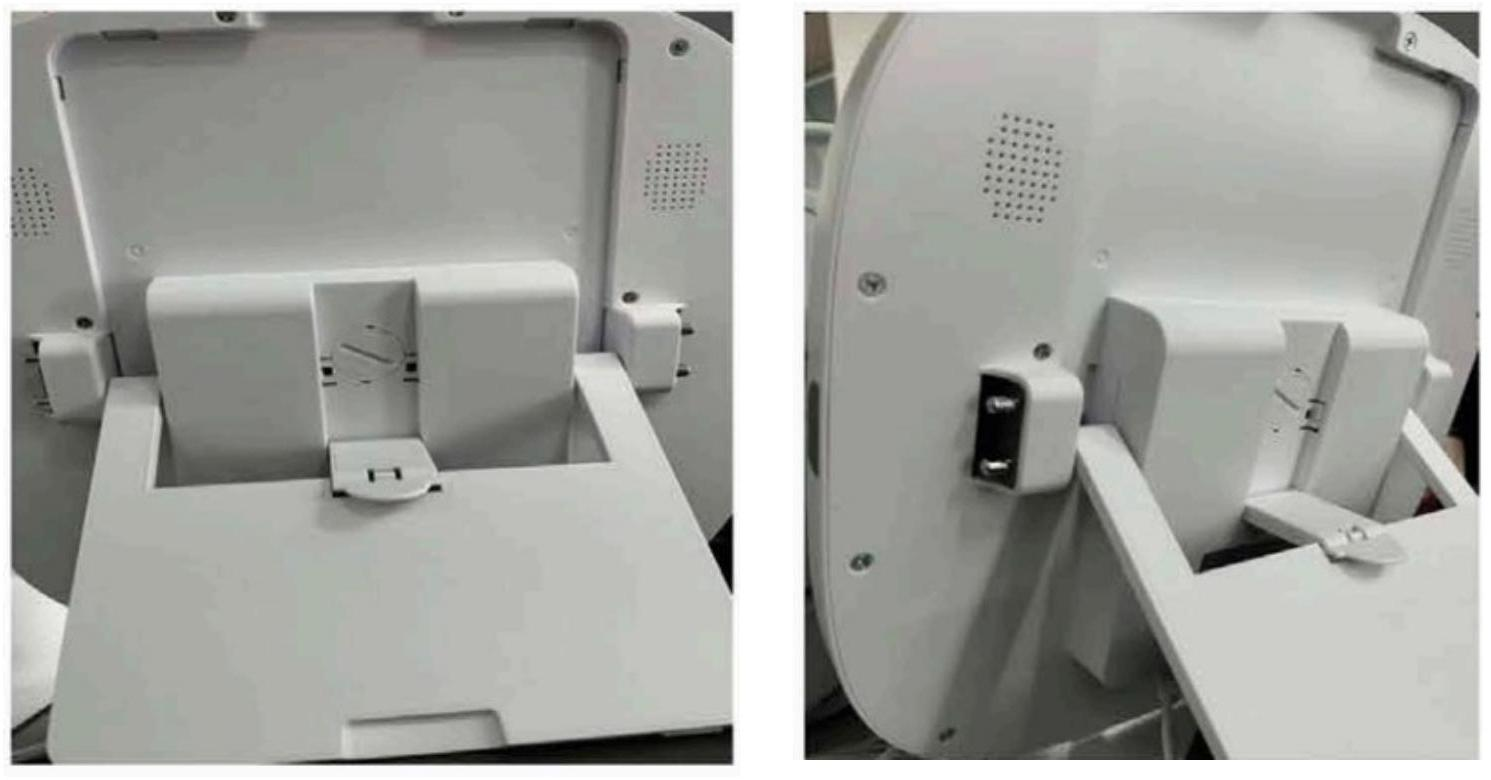
\includegraphics[alt={},max width=\textwidth]{018f02f8-3740-46eb-ab06-ecd68977d8ca-05_780_1491_1544_290}
\captionsetup{labelformat=empty}
\caption{Immagine 3-3}
\end{center}
\end{figure}

\begin{enumerate}
  \setcounter{enumi}{2}
  \item Premi a lungo il pulsante di accensione sul lato destro del tablet per $3-4$ secondi per accenderlo; e clicca sul pulsante di regolazione della luce sul lato sinistro per regolare 3 tipi di lluminazione;
\end{enumerate}

\section{Introduzione all'interfaccia}
\subsection{Introduzione della pagina iniziale}
Fai clic sull'app per accedere al sistema di analisi. Come mostrato nella figura 4-1-1

\begin{figure}[H]
\begin{center}
  
\includegraphics[alt={},max width=\textwidth]{018f02f8-3740-46eb-ab06-ecd68977d8ca-05_893_666_752_2811}
\captionsetup{labelformat=empty}
\caption{Immagine 4-1-1}
\end{center}
\end{figure}

\subsubsection{Pagina pubblicitaria}
Dopo aver acceso l'apparecchio, l'interfaccia passerà automaticamente all'interfaccia di pubblicità del software (come mostrato nella Figura 4-1-2).\\
Si tratta di un display pubblicitario, utilizzato principalmente per promuovere i prodotti o gli strumenti del negozio, ma che può anche servire a mostrare offerte promozionali per attirare i clienti e farli scoprire i dettagli dei prodotti.\\
Puoi modificare l'immagine pubblicitaria da visualizzare: clicca su qualsiasi angolo dello schermo per accedere alla

Sistema.

\section{OEM Multiple oltre ogni tua immaginazione}
Analizzare con precisione il marketing scientifico

\begin{figure}[H]
\begin{center}
  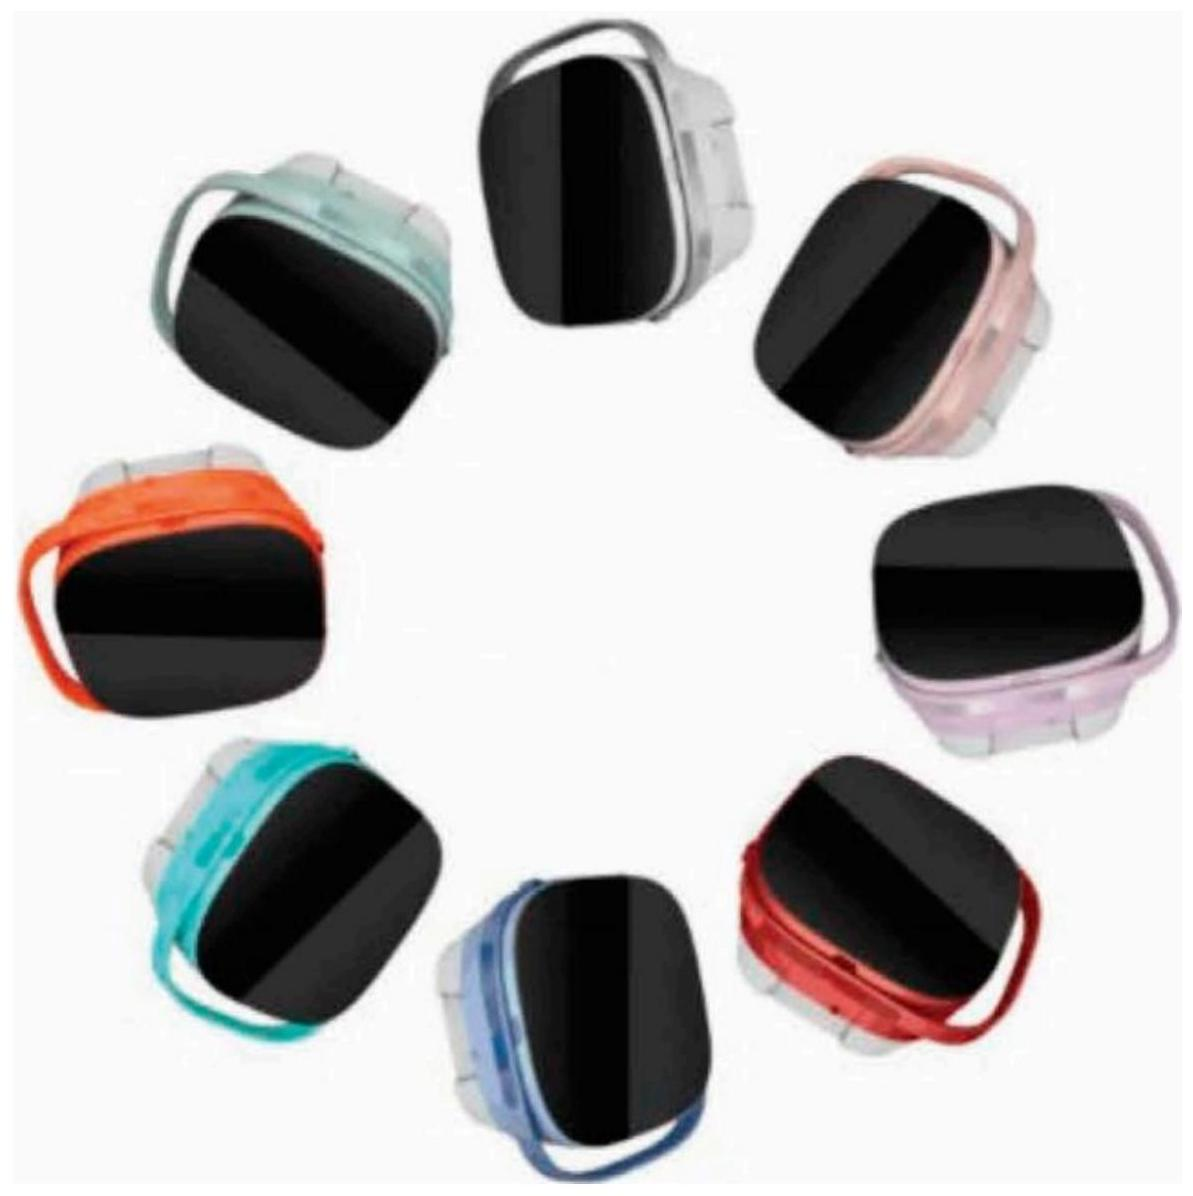
\includegraphics[alt={},max width=\textwidth]{018f02f8-3740-46eb-ab06-ecd68977d8ca-06_1196_1193_788_426}
\captionsetup{labelformat=empty}
\caption{Immagine 4-1-2}
\end{center}
\end{figure}

\subsubsection{Barra degli strumenti}
Una volta acceduto al software, l'interfaccia principale comprende principalmente i seguenti elementi: la barra degli strumenti, la sezione del logo, la barra di ricerca per le informazioni clienti, la sezione per i nuovi clienti, la pagina di ritorno alla pagina pubblicitaria e l' interfaccia di gestione del negozio.

\begin{figure}[H]
\begin{center}
  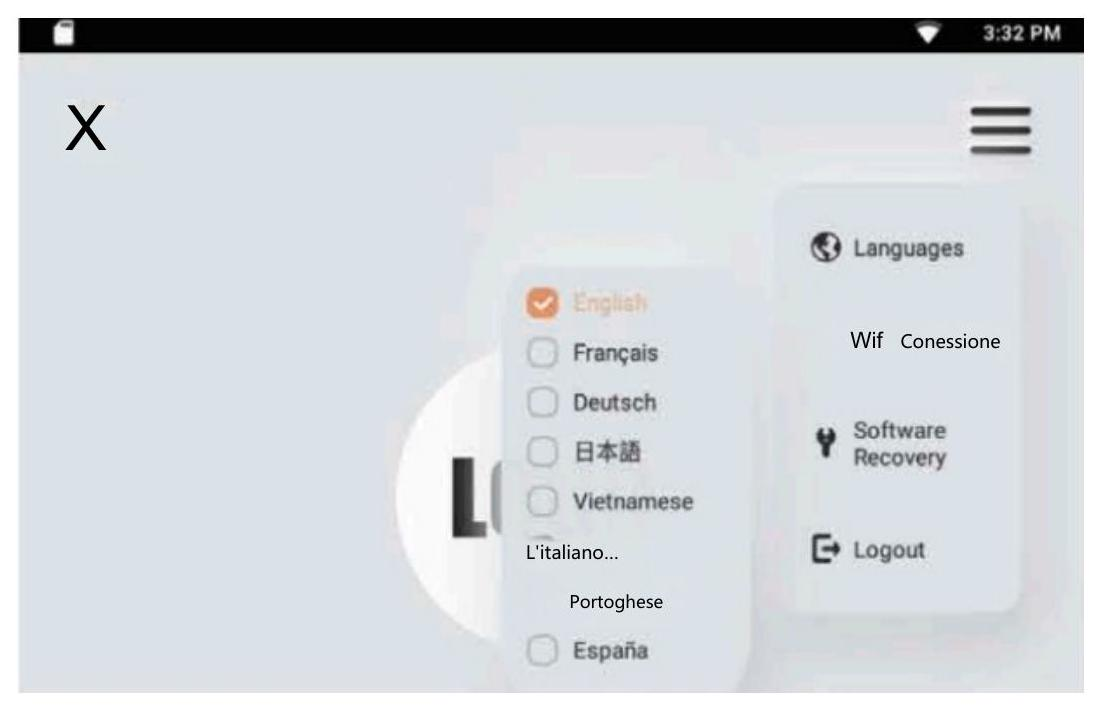
\includegraphics[alt={},max width=\textwidth]{018f02f8-3740-46eb-ab06-ecd68977d8ca-06_708_1096_193_2547}
\captionsetup{labelformat=empty}
\caption{Immagine 4-1-3}
\end{center}
\end{figure}

Come mostrato nella figura 4-1-3, clicca per accedere alla barra degli strumenti:\\
Scegliere la lingua: 7 lingue sono opzionali (inglese, francese, tedesco, giapponese, vietnamita, italiana, portoghese, spagnolo)\\
Conessione Wi-Fi:Inserisci le informazioni del Wi-Fi per connettersi al Wi-Fi disponibile in negozio o al Wi-Fi degli apparecchi (LDwifi), come mostrato nella figura 4-1-4\\
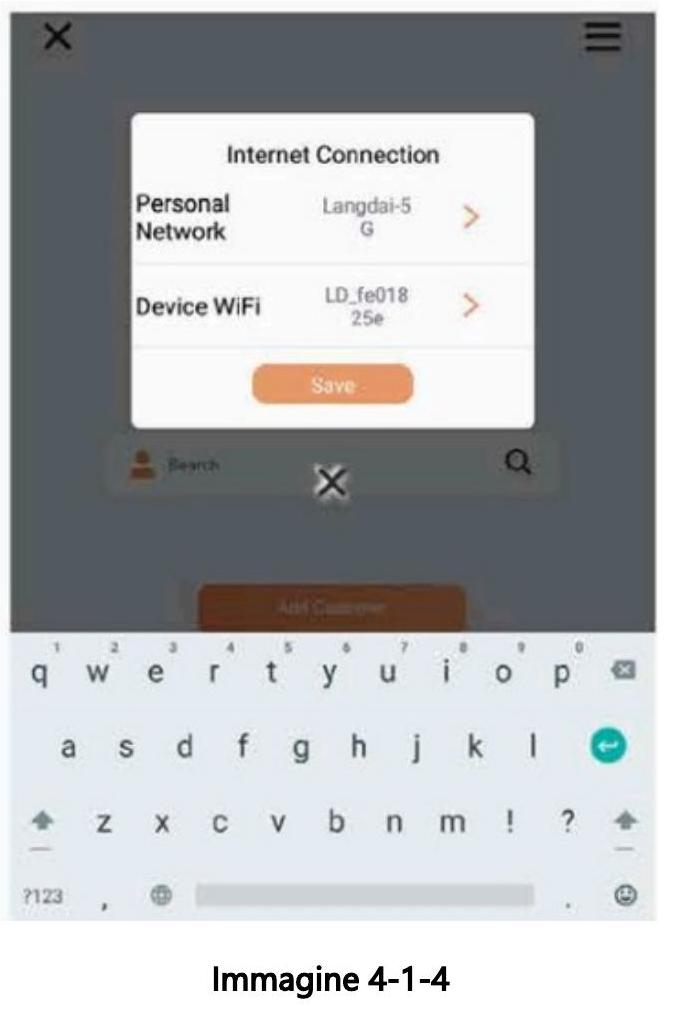
\includegraphics[max width=\textwidth, alt={}, center]{018f02f8-3740-46eb-ab06-ecd68977d8ca-06_1009_673_1635_2769}

Riparazione del software: utilizzato principalmente per l'aggiornamento e la riparazione del software.\\
Uscita:Esce dall'interfaccia del software Camface e torna alla barra degli strumenti dell'app del sistema.

\subsubsection{Pagina iniziale}
Come mostrato nella Figura 4-1-4:\\
LOGO:Puoi inserire il tuo logo qui (vedi 7.3.2 per i dettagli)\\
Barra di ricerca:Trova rapidamente i clienti cercando i loro nomi e numeri di telefono.Aggiungi cliente: Crea file clienti e aggiungi nuove informazioni sui clienti. (come mostrato nella Figura 4-1-5)

Inserisci prima le informazioni necessarie: nome, sesso, data di nascita e numero di telefono.

Inserisci poi altre informazioni: storia di allergie, principali problemi cutanei che hai avuto e prodotti in uso.

\begin{figure}[H]
\begin{center}
  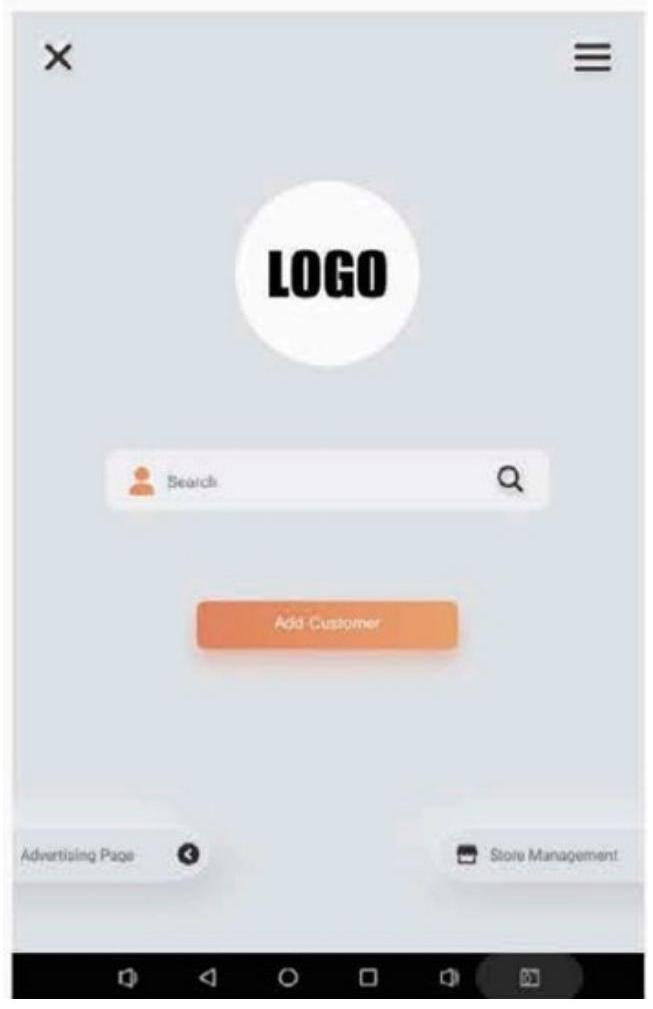
\includegraphics[alt={},max width=\textwidth]{018f02f8-3740-46eb-ab06-ecd68977d8ca-07_1009_653_1557_352}
\captionsetup{labelformat=empty}
\caption{Immagine 4-1-4}
\end{center}
\end{figure}

Infine, fai clic su "Salva" o su "Salva e effettua l'analisi della pelle".

\begin{figure}[H]
\begin{center}
  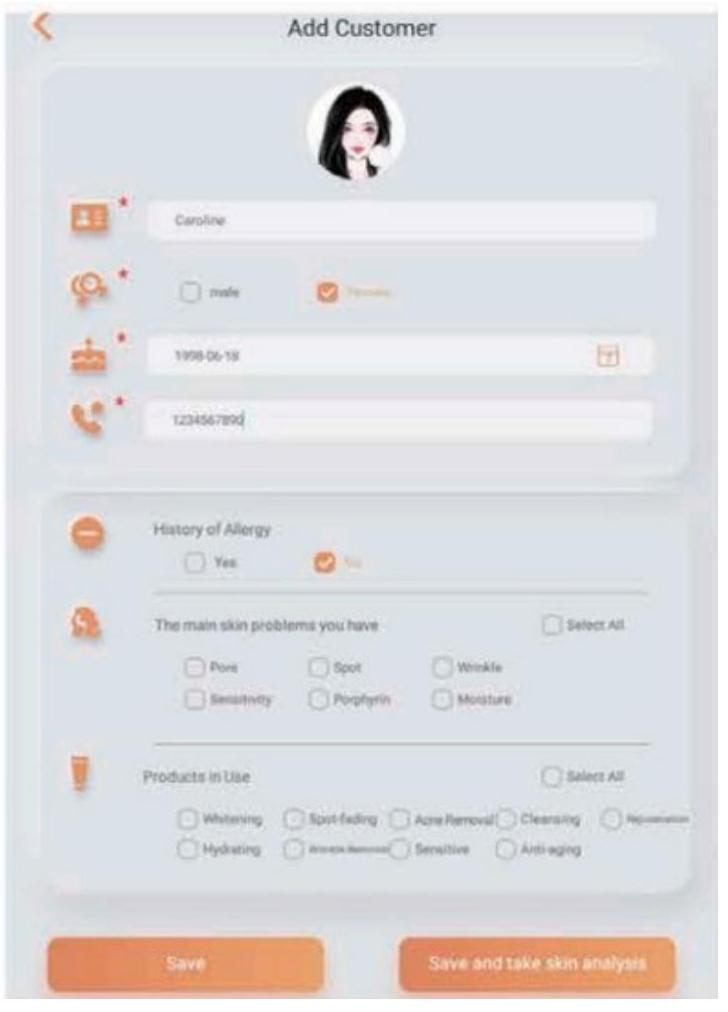
\includegraphics[alt={},max width=\textwidth]{018f02f8-3740-46eb-ab06-ecd68977d8ca-07_1012_728_1557_1092}
\captionsetup{labelformat=empty}
\caption{Immagine 4-1-5}
\end{center}
\end{figure}

Pagina pubblicitaria:Clicca su " Pagina pubblicitaria " per tornare all' interfaccia di visualizzazione delle pubblicità (come mostrato nella Figura 4-1-2). L' interfaccia pubblicitaria consente di inserire immagini o video (per maggiori dettagli, consultare le sezioni 6.4 .6 e 7.3.2).

Gestione del negozio:Accedi alla sezione Gestione File Clienti/Gestione Dati/Gestione Prodotti/Impostazioni come mostrato nella Figura 4-1-6.

\begin{figure}[H]
\begin{center}
  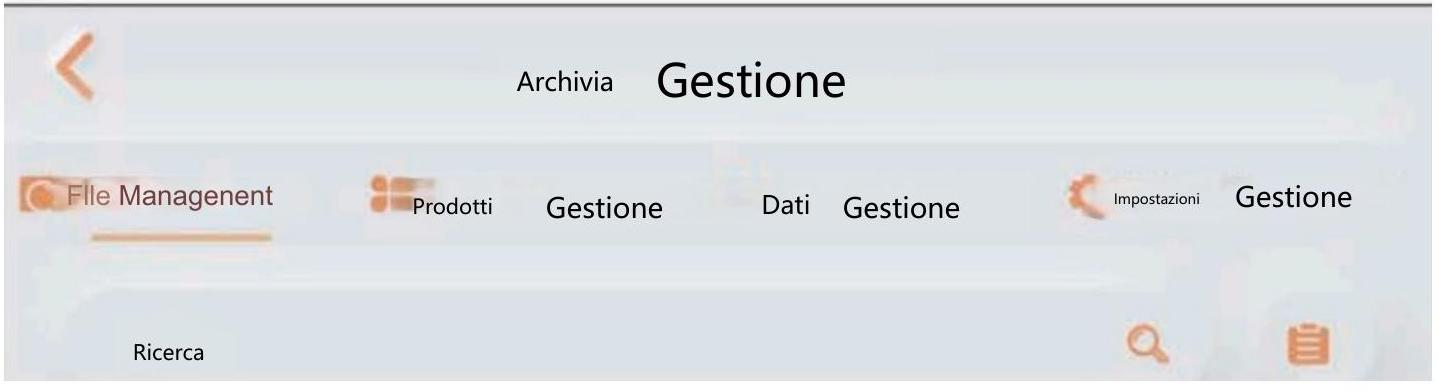
\includegraphics[alt={},max width=\textwidth]{018f02f8-3740-46eb-ab06-ecd68977d8ca-07_392_1439_775_2381}
\captionsetup{labelformat=empty}
\caption{Immagine 4-1-6}
\end{center}
\end{figure}

\subsubsection{Introduzione di altre chiavi}
Come mostrato nella figura 4-1-7, dall'indietro a destra si trovano: "volume-", "torna alla pagina precedente", "interfaccia home screen", "Split Screen", "volume+" e "screenshot".\\
□\\
口

\section{Guida all'operazione}
\subsection{Fotografie}
Una volta aggiunto con successo il cliente, puoi cliccare direttamente per salvare e iniziare l'analisi della pelle (come mostrato nella Figura 4-1-5); oppure cliccare per iniziare a scattare le foto, come mostrato nella Figura 5-1-1.

\begin{figure}[H]
\begin{center}
  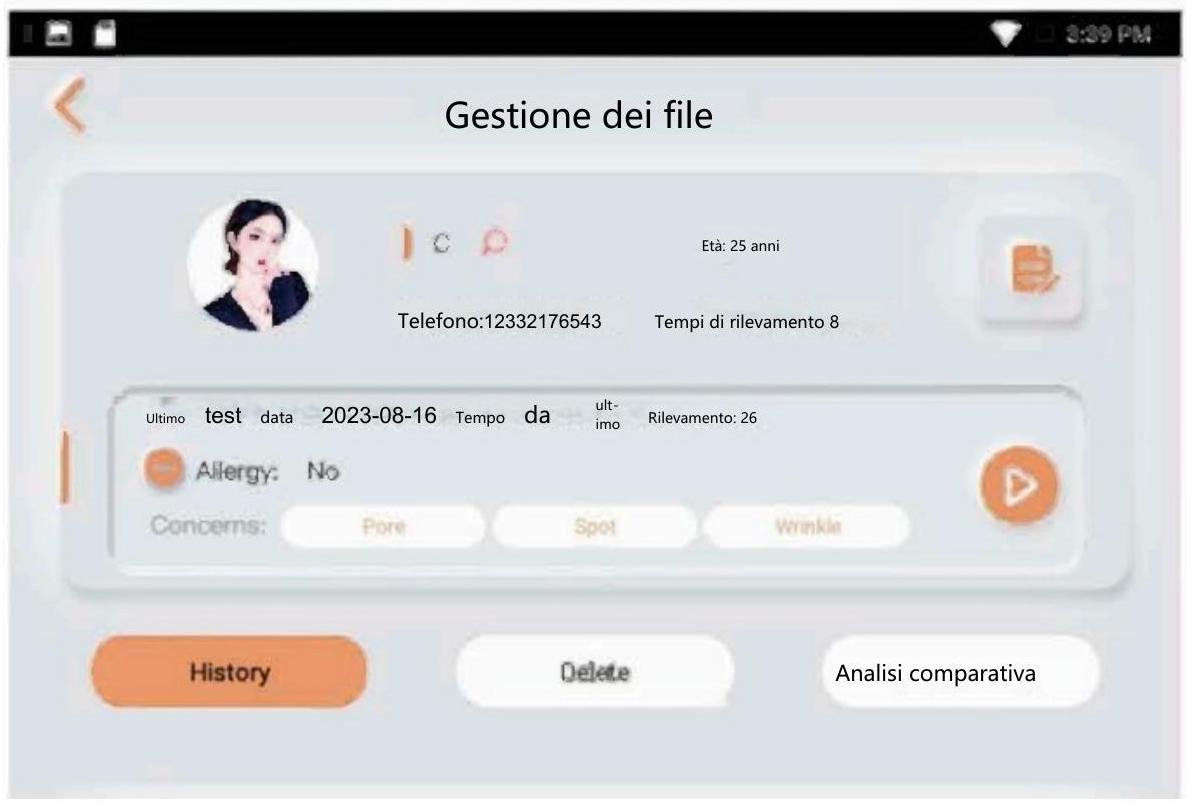
\includegraphics[alt={},max width=\textwidth]{018f02f8-3740-46eb-ab06-ecd68977d8ca-08_805_1193_730_439}
\captionsetup{labelformat=empty}
\caption{Immagine 5-1-1}
\end{center}
\end{figure}

\section{Consigli prima di scattare:}
\begin{enumerate}
  \item Angolo di ripresa: assicurati di guardare in avanti, chiudere gli occhi e non guardare in basso, in alto o di lato.
  \item Evitare la luce esterna: durante la ripresa è necessario abbassare la copertura ogni volta per evitare l'influenza di fonti luminose esterne. Assicurarsi che non ci siano capelli in eccesso sul viso che possano entrare nell'area di regolazione, posizionare il viso nel supporto del mento e nel supporto della fronte, quindi premere il pulsante di ripresa per avviare l'analisi.
  \item Senza trucco: il creme corretto, la base e altri prodotti funzionali coprono le imperfezioni superficiali della pelle, mentre la protezione solare blocca i raggi UV che potrebbero danneggiare il viso. Assicurati di non truccare la pelle durante la ripresa per ottenere risultati di analisi accurati; quindi fai clic, come mostrato in figura 5-1-25-1-3.
\end{enumerate}

\begin{figure}[H]
\begin{center}
  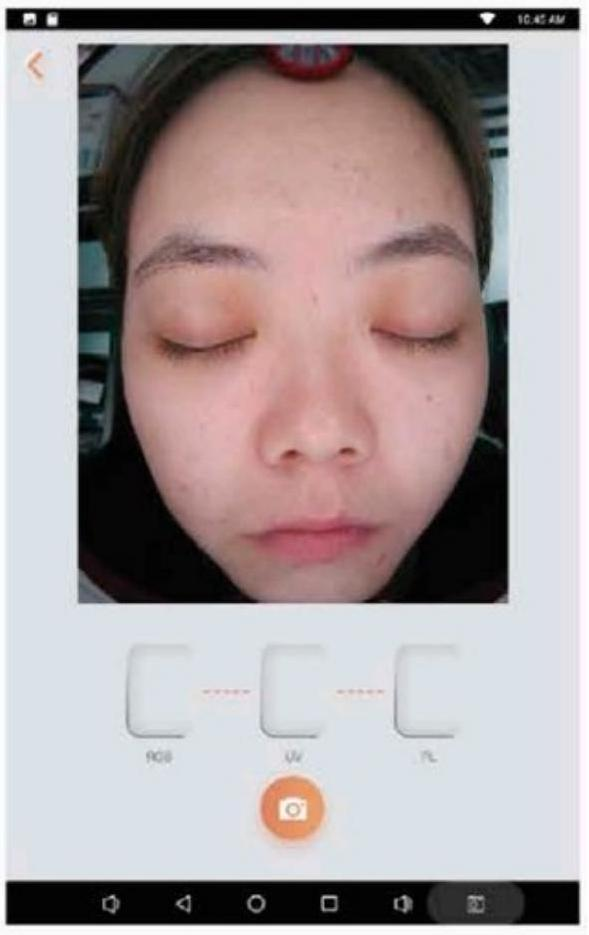
\includegraphics[alt={},max width=\textwidth]{018f02f8-3740-46eb-ab06-ecd68977d8ca-08_935_589_193_2481}
\captionsetup{labelformat=empty}
\caption{Immagine 5-1-2}
\end{center}
\end{figure}

\begin{figure}[H]
\begin{center}
  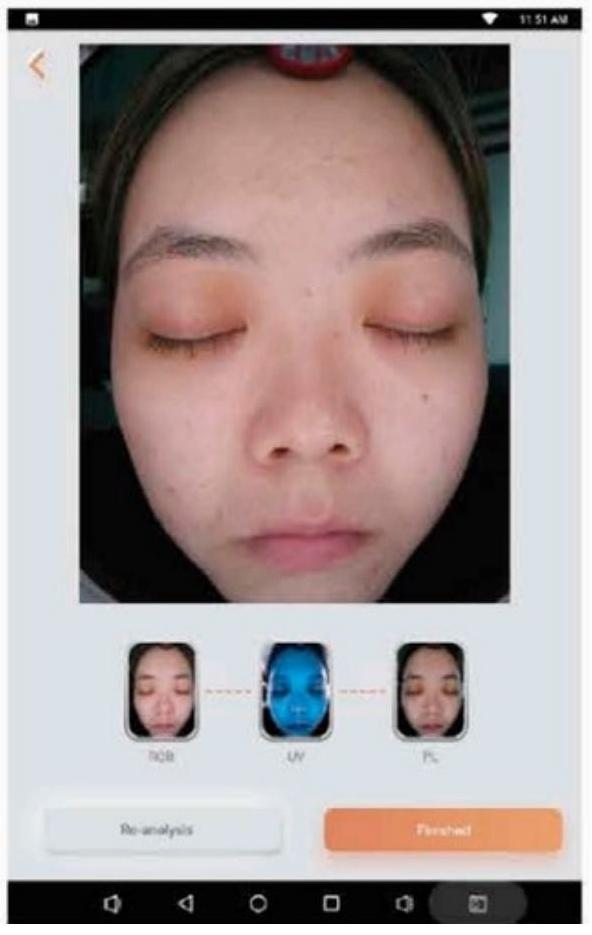
\includegraphics[alt={},max width=\textwidth]{018f02f8-3740-46eb-ab06-ecd68977d8ca-08_935_592_193_3134}
\captionsetup{labelformat=empty}
\caption{Immagine 5-1-3}
\end{center}
\end{figure}

\begin{figure}[H]
\begin{center}
  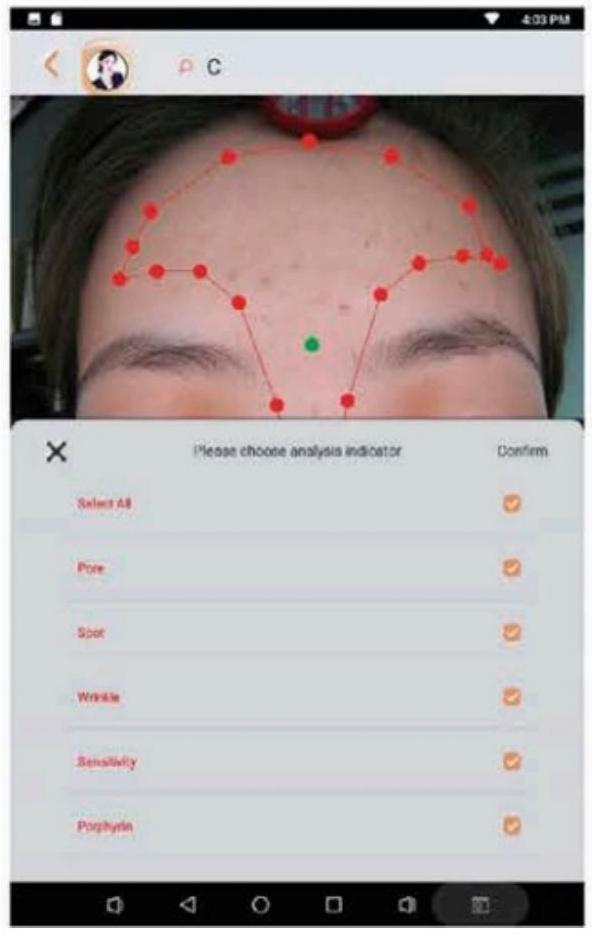
\includegraphics[alt={},max width=\textwidth]{018f02f8-3740-46eb-ab06-ecd68977d8ca-08_938_592_1657_2462}
\captionsetup{labelformat=empty}
\caption{Immagine 5-1-4}
\end{center}
\end{figure}

\begin{figure}[H]
\begin{center}
  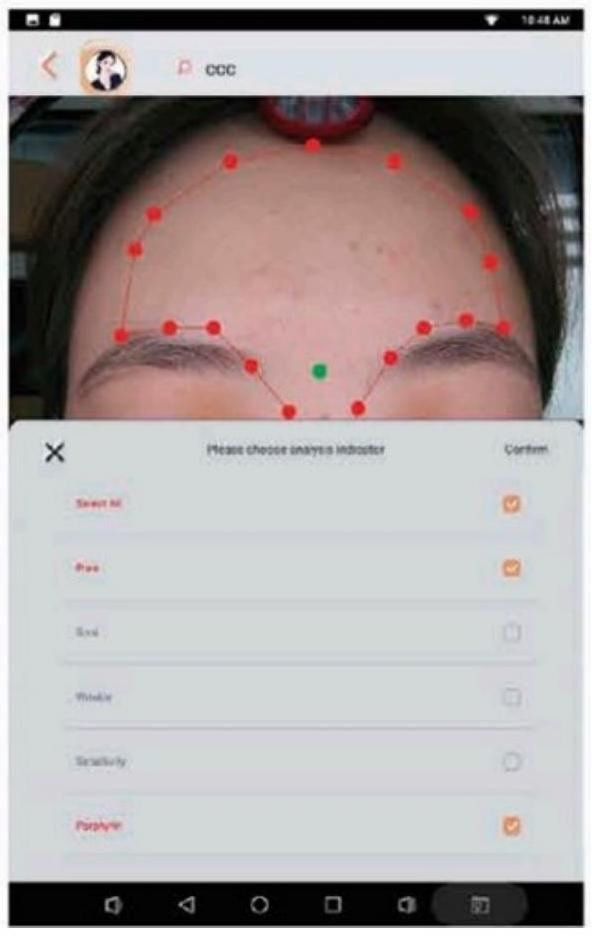
\includegraphics[alt={},max width=\textwidth]{018f02f8-3740-46eb-ab06-ecd68977d8ca-08_938_592_1657_3121}
\captionsetup{labelformat=empty}
\caption{Immagine 5-1-5}
\end{center}
\end{figure}

Clicca e controllare l'analisi della pelle regolabile dopo la scattatura, come mostrato nella figura $5-1-45-1-5$. I parametri predefiniti includono l'analisi di 6 problemi cutanei; è possibile personalizzare gli elementi di analisi in base alle esigenze, quindi clicca su L'elemento di analisi personalizzato apparirà in un singolo rapporto, come mostrato nella figura 5-1-6 5-1-7.

\begin{figure}[H]
\begin{center}
  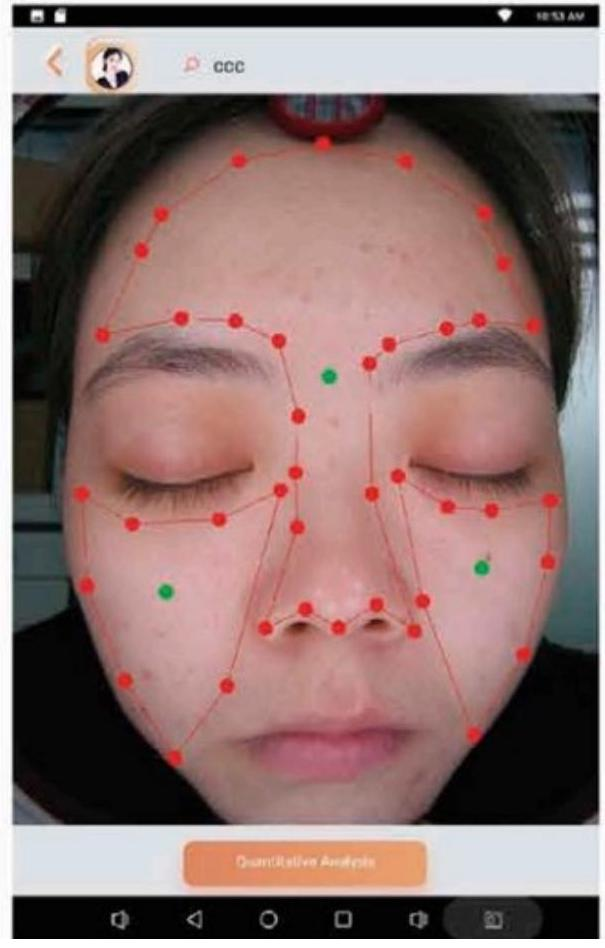
\includegraphics[alt={},max width=\textwidth]{018f02f8-3740-46eb-ab06-ecd68977d8ca-09_948_605_213_355}
\captionsetup{labelformat=empty}
\caption{Immagine 5-1-6}
\end{center}
\end{figure}

\begin{figure}[H]
\begin{center}
  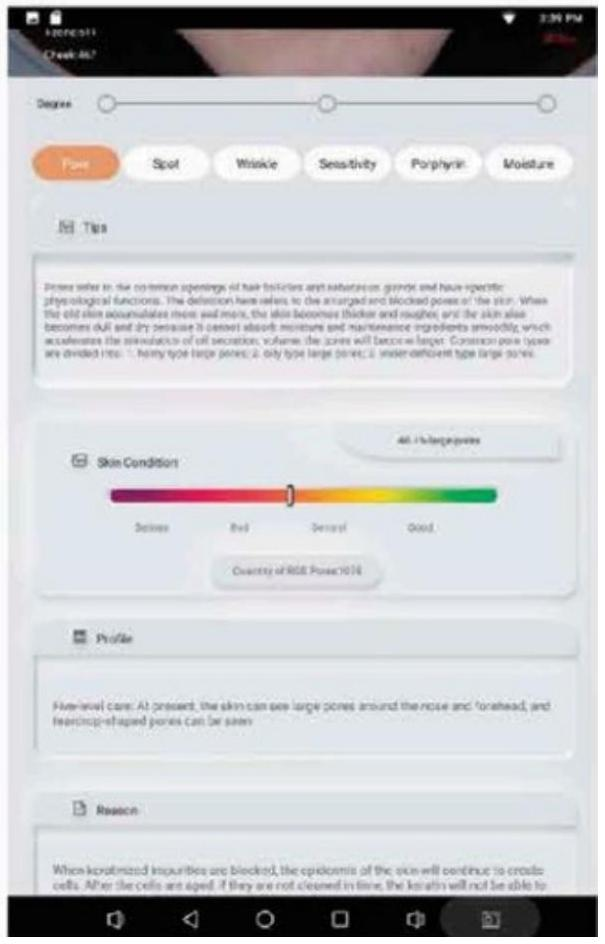
\includegraphics[alt={},max width=\textwidth]{018f02f8-3740-46eb-ab06-ecd68977d8ca-09_944_605_213_1066}
\captionsetup{labelformat=empty}
\caption{Immagine 5-1-7}
\end{center}
\end{figure}

\begin{figure}[H]
\begin{center}
  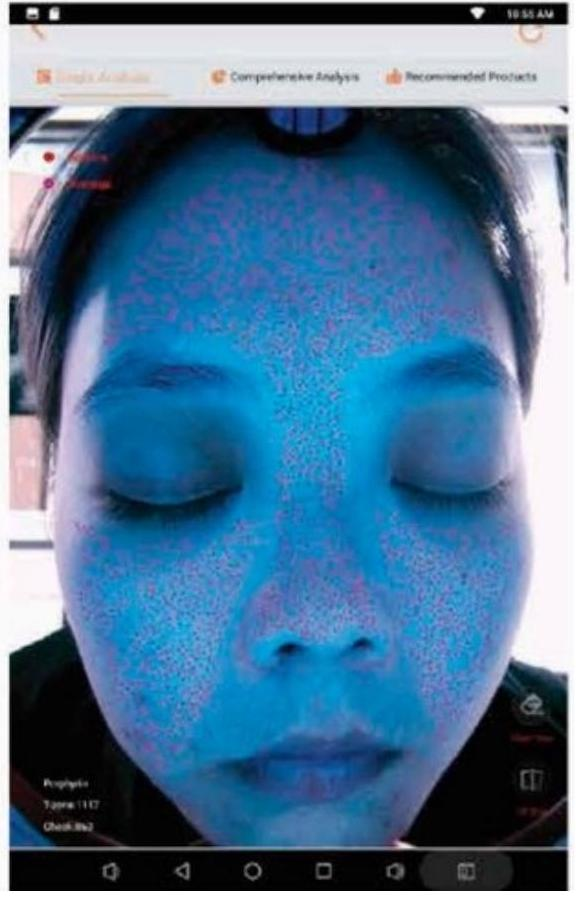
\includegraphics[alt={},max width=\textwidth]{018f02f8-3740-46eb-ab06-ecd68977d8ca-09_899_576_1693_371}
\captionsetup{labelformat=empty}
\caption{Immagine 5-2-1}
\end{center}
\end{figure}

\begin{figure}[H]
\begin{center}
  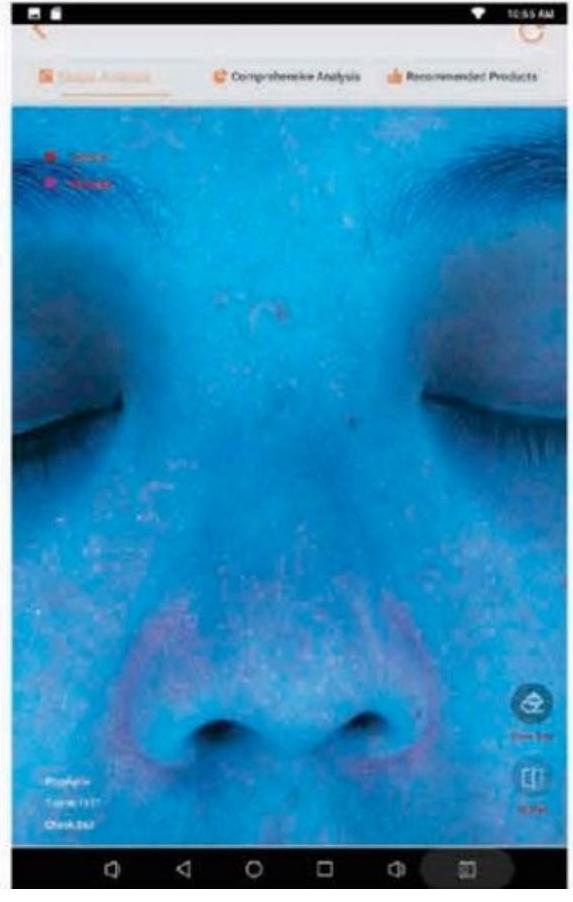
\includegraphics[alt={},max width=\textwidth]{018f02f8-3740-46eb-ab06-ecd68977d8ca-09_902_573_1693_1053}
\captionsetup{labelformat=empty}
\caption{Immagine 5-2-2}
\end{center}
\end{figure}

\subsection{Analisi singola}
Come mostrato nella figura 5-2-1, seleziona gli elementi dell'analisi della pelle in base alle tue esigenze; quindi, premi due dita sullo schermo e scorrili per ingrandire l'immagine e visualizzare i dettagli, come illustrato nella figura 5-2-2.

\begin{figure}[H]
\begin{center}
  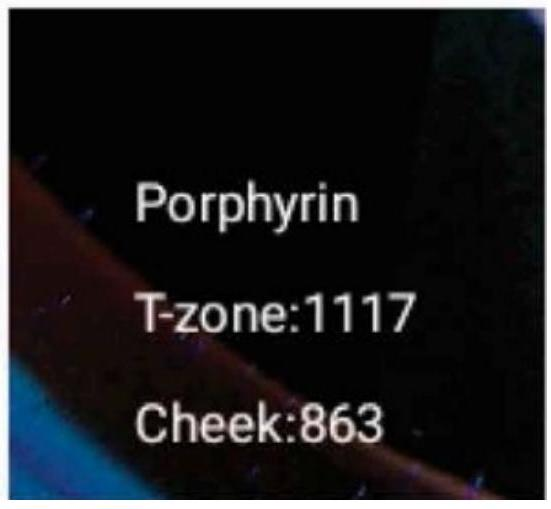
\includegraphics[alt={},max width=\textwidth]{018f02f8-3740-46eb-ab06-ecd68977d8ca-09_509_551_432_2429}
\captionsetup{labelformat=empty}
\caption{Immagine 5-2-3}
\end{center}
\end{figure}

\begin{figure}[H]
\begin{center}
  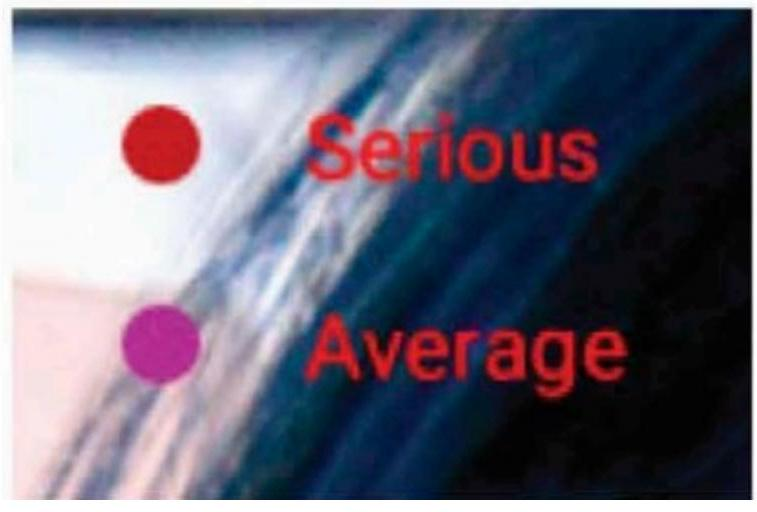
\includegraphics[alt={},max width=\textwidth]{018f02f8-3740-46eb-ab06-ecd68977d8ca-09_512_757_432_3014}
\captionsetup{labelformat=empty}
\caption{Immagine 5-2-4}
\end{center}
\end{figure}

\begin{figure}[H]
\begin{center}
  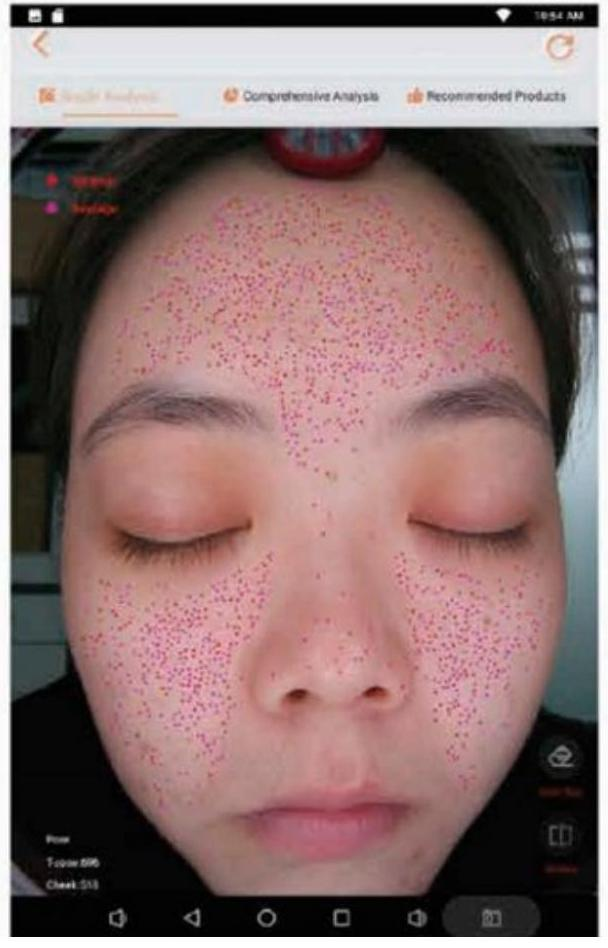
\includegraphics[alt={},max width=\textwidth]{018f02f8-3740-46eb-ab06-ecd68977d8ca-09_948_608_1570_2436}
\captionsetup{labelformat=empty}
\caption{Immagine 5-2-5}
\end{center}
\end{figure}

\begin{figure}[H]
\begin{center}
  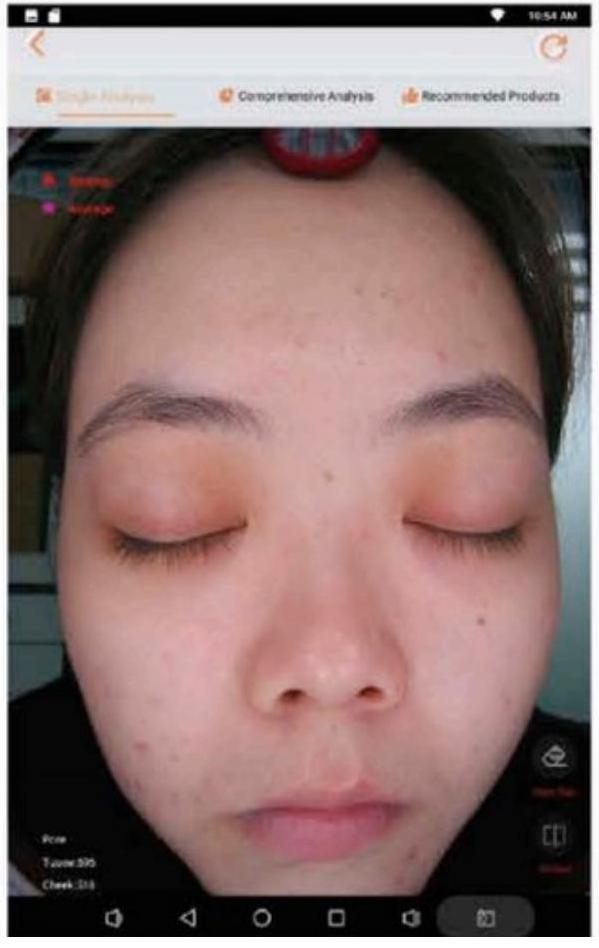
\includegraphics[alt={},max width=\textwidth]{018f02f8-3740-46eb-ab06-ecd68977d8ca-09_948_599_1570_3153}
\captionsetup{labelformat=empty}
\caption{Immagine 5-2-6}
\end{center}
\end{figure}

Zona T e guance:I numeri nell' angolo in basso a sinistra dell' immagine corrispondono rispettivamente al numero di problemi relativi alla zona T e alle guance, come mostrato nell' immagine 5-2 3 .

Colori dei marcatori:l diversi colori dei marcatori nell'angolo in alto a sinistra indicano diversi gradi di problemi cutanei, come mostrato nella figura 5-2 - 4

Tag puliti:Clicca per rimuovere il segno di problema e visualizzarlo meglio sulla pelle mostrato nella figura 5-2-55-2-6.

Come illustrato nella figura 5-2-7, sono presenti 9 analisi singole, tra cui macchie, pigmentazione, aree brune e danni UV sono riassunte in una sezione

Alla fine di un'analisi, clicca su\\
localmente. (Come mostrato nella figura 5-2-8) apposita, che rientra nel rapporto completo sulle macchie.\\
per salvare il rapporto.

\begin{figure}[H]
\begin{center}
  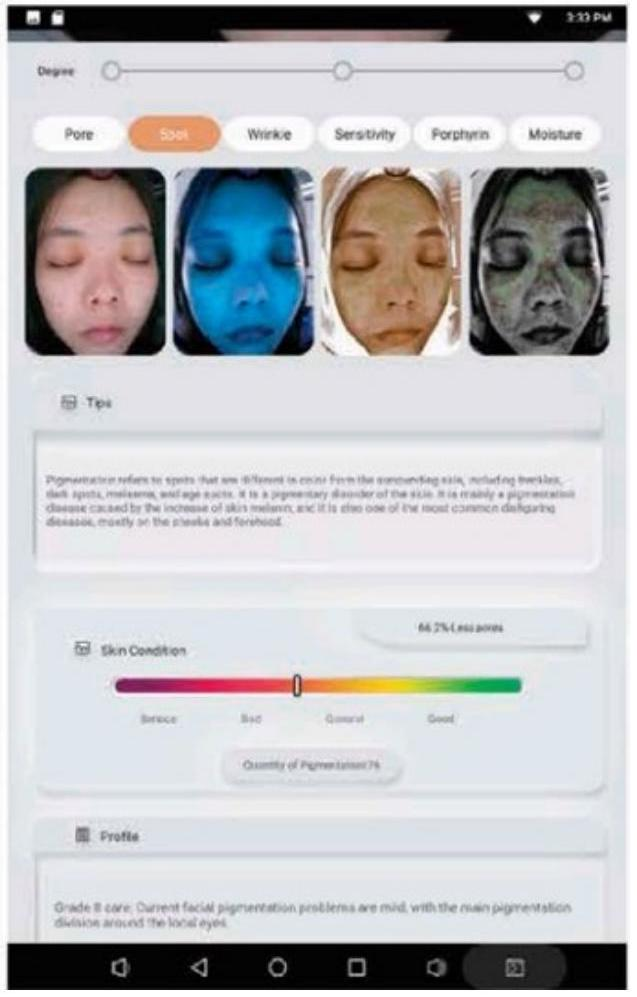
\includegraphics[alt={},max width=\textwidth]{018f02f8-3740-46eb-ab06-ecd68977d8ca-10_997_637_781_336}
\captionsetup{labelformat=empty}
\caption{Immagine 5-2-7}
\end{center}
\end{figure}

\begin{figure}[H]
\begin{center}
  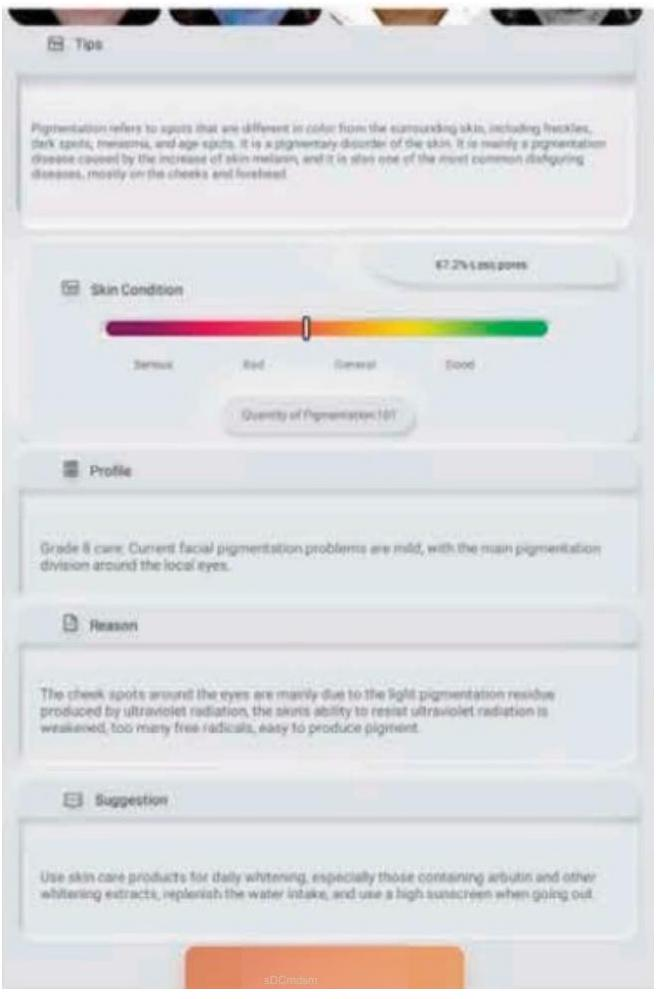
\includegraphics[alt={},max width=\textwidth]{018f02f8-3740-46eb-ab06-ecd68977d8ca-10_999_656_775_1034}
\captionsetup{labelformat=empty}
\caption{Immagine 5-2-8}
\end{center}
\end{figure}

Nota: Il valore percentuale si basa sul confronto con persone della stessa fascia d'età.\\
Più alto è il valore, migliore è la condizione della tua pelle.\\
Pore RGB: indica la presenza di pori di grandi dimensioni sulla pelle superficiale, ovvero pori di diametro superiore a $0,02-0,05 \mathrm{~mm}$.\\
Spot RGB: indica un punto cutaneo attuale il cui colore è più scuro del colore normale della pelle e che presenta una forma rotonda o irregolare sulla superficie cutanea.\\
Pigmentazione UV: indica la pigmentazione attuale della derma, che prevede la comparsa futura di macchie superficiali; alcune aree più gravi sono già visibili, e più è scura, peggio è la situazione, richiedendo maggiore attenzione.\\
Area marrone: indica lo stato del metabolismo cutaneo; per alcune persone è necessario

\begin{figure}[H]
\begin{center}
  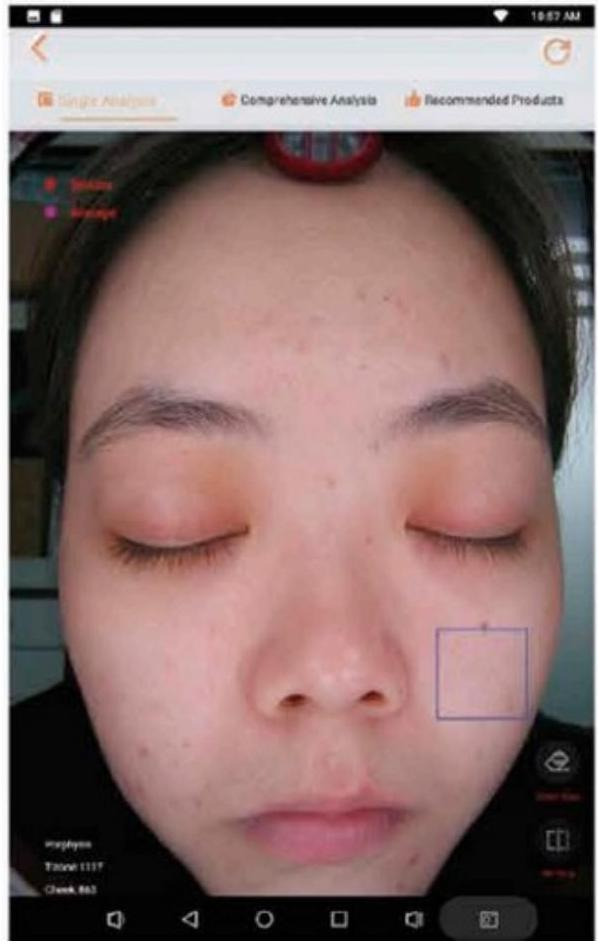
\includegraphics[alt={},max width=\textwidth]{018f02f8-3740-46eb-ab06-ecd68977d8ca-10_948_598_1641_2475}
\captionsetup{labelformat=empty}
\caption{Immagine 5-3-1}
\end{center}
\end{figure}

\begin{figure}[H]
\begin{center}
  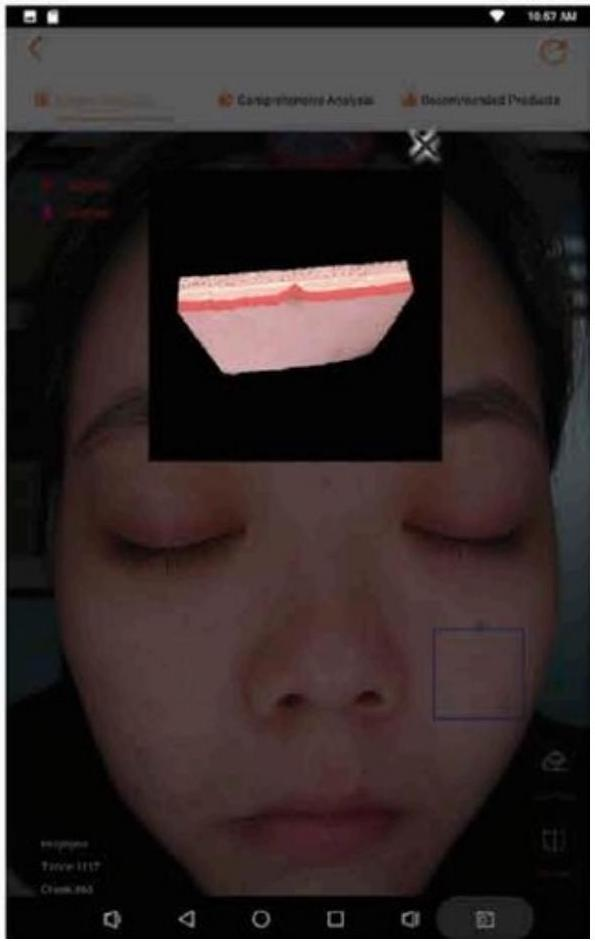
\includegraphics[alt={},max width=\textwidth]{018f02f8-3740-46eb-ab06-ecd68977d8ca-10_941_595_1641_3173}
\captionsetup{labelformat=empty}
\caption{Immagine 5-3-2}
\end{center}
\end{figure}

Il metabolismo non è ottimo: da quelle macchie marroni si possono vedere le aree interessate.\\
Lesione da UV: si tratta di una macchia nella pelle profonda causata da un' esposizione prolungata al sole, da un uso insufficiente del filtro solare e da bruciature solari, che alla fine portano a una pigmentazione grave nelle zone più interne della pelle.\\
Righe RGB: indica lo stato attuale delle rughe e l'area della pelle non liscia né piana; pi ù alto è il valore percentuale, migliore è la condizione delle rughe. Area sensibile: indica uno stato di pelle particolarmente reattiva, soggetta a allergie in caso di cambiamento delle stagioni o all'uso di cosmetici contenenti metalli pesanti in quantit à eccessiva.

UV Porphyrin: indica la secrezione di sebo nella derma e la presenza di comedoni. UV Moisture: indica lo stato di umidità della pelle nella derma.

\subsection{3 "Slice 3D"}

\includegraphics[max width=\textwidth, alt={}]{018f02f8-3740-46eb-ab06-ecd68977d8ca-10_62_1626_1441_2255} vedi l'immagine 3D per i problemi della pelle.

\subsection{Rapporto completo}
\begin{verbatim}
Comprehensive Analysis C
\end{verbatim}

icca ingresso nella figura 5-4-1 5-4-2, che mostra il risultato dell'analisi completa e la simulazione dell'età della pelle. La tabella di valutazione mostra le condizioni cutanee in confronto a persone della stessa fascia d'età. "Tipo di Pelle Attuale" mostra automaticamente il tipo di pelle in base ai risultati dell'analisi. Le raccomandazioni per la cura della pelle possono essere modificate tramite Cloud, personalizzabili in base alle esigenze del mercato locale (vedi 7.3.4 per i dettagli). e\\

\includegraphics[max width=\textwidth, alt={}, center]{018f02f8-3740-46eb-ab06-ecd68977d8ca-11_76_405_836_1363}

Alla fine dell'analisi completa, clicca su

\begin{figure}[H]
\begin{center}
  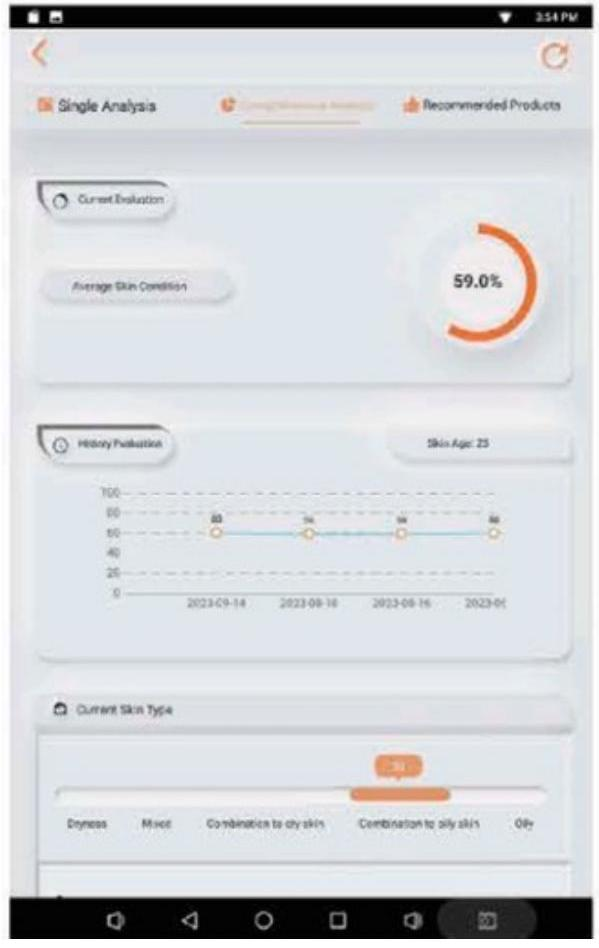
\includegraphics[alt={},max width=\textwidth]{018f02f8-3740-46eb-ab06-ecd68977d8ca-11_948_599_1059_400}
\captionsetup{labelformat=empty}
\caption{Immagine 5-4-1}
\end{center}
\end{figure}

Carica nel cloud per salvare il rapporto nel cloud o sul dispositivo locale. (Come mostrato nella figura 5-4-2)

\begin{figure}[H]
\begin{center}
  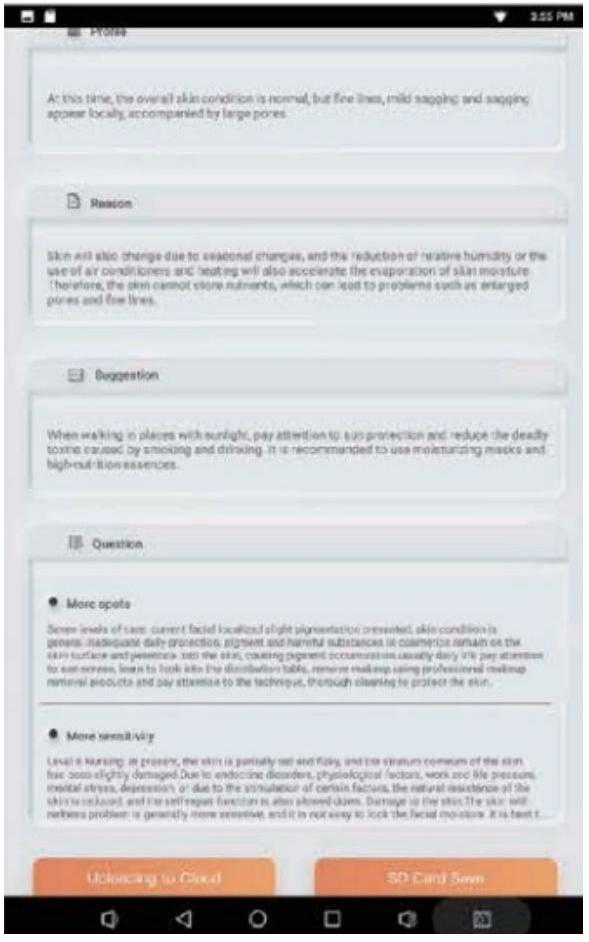
\includegraphics[alt={},max width=\textwidth]{018f02f8-3740-46eb-ab06-ecd68977d8ca-11_942_589_1059_1072}
\captionsetup{labelformat=empty}
\caption{Immagine 5-4-2}
\end{center}
\end{figure}

\subsection{Prodotti consigliati}
La sezione "Prodotti consigliati" viene generata automaticamente dal sistema in base allo stato della pelle del cliente, fornendo prodotti già pre-downloaded nella sezione "Prodotti" del cloud (vedi 7.2.3 per i dettagli). È inoltre possibile aggiungere o eliminare prodotti per la cura della pelle in base alle esigenze del cliente, come mostrato nelle figure 5-5-1 e 5-5-2.

\begin{figure}[H]
\begin{center}
  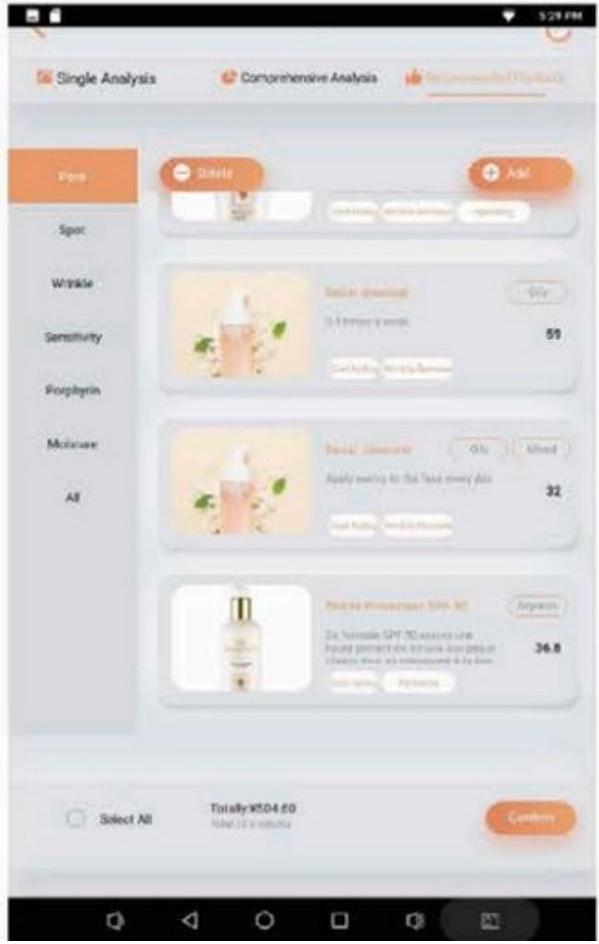
\includegraphics[alt={},max width=\textwidth]{018f02f8-3740-46eb-ab06-ecd68977d8ca-11_944_599_213_2536}
\captionsetup{labelformat=empty}
\caption{Immagine 5-5-1}
\end{center}
\end{figure}

\begin{figure}[H]
\begin{center}
  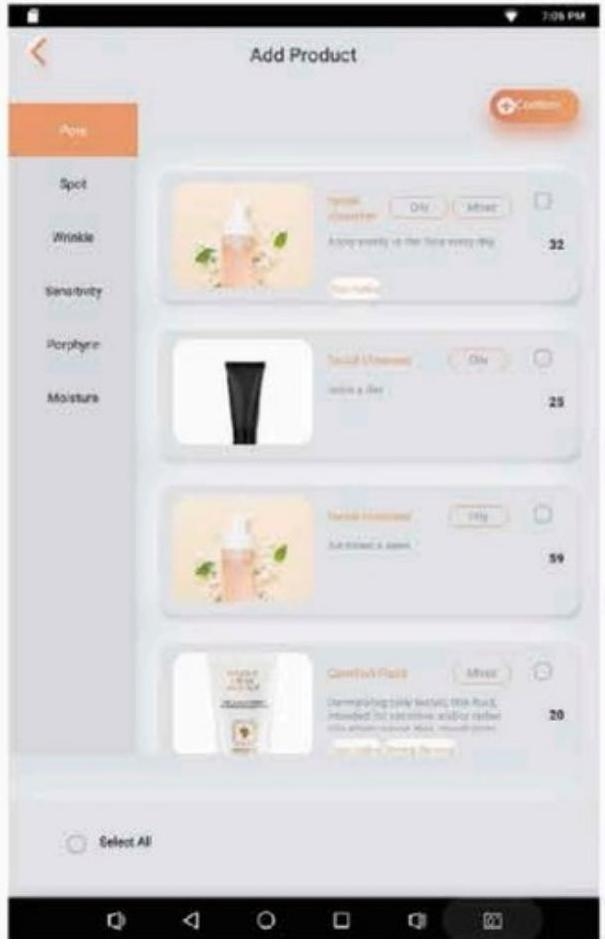
\includegraphics[alt={},max width=\textwidth]{018f02f8-3740-46eb-ab06-ecd68977d8ca-11_944_605_213_3234}
\captionsetup{labelformat=empty}
\caption{Immagine 5-5-2}
\end{center}
\end{figure}

\begin{figure}[H]
\begin{center}
  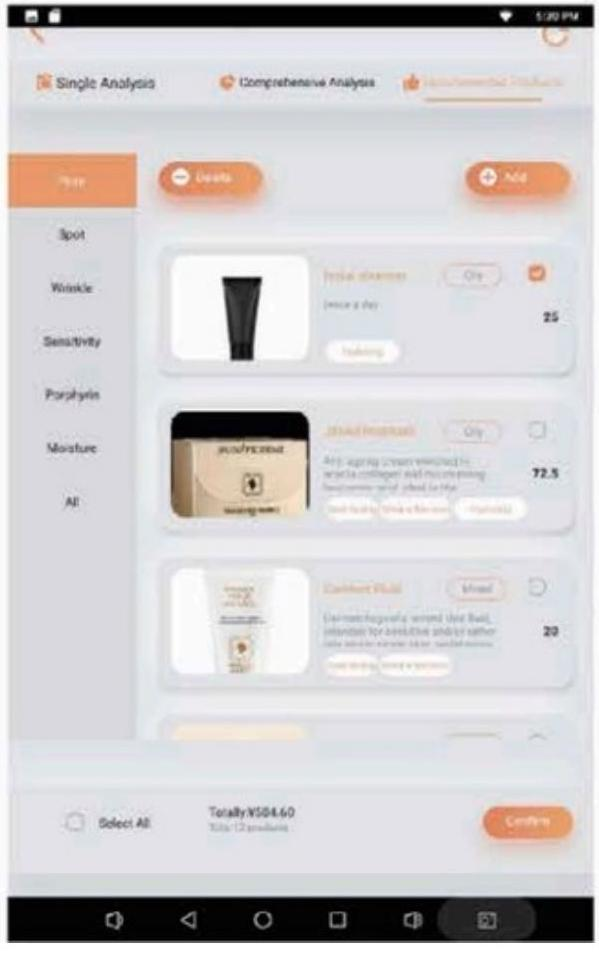
\includegraphics[alt={},max width=\textwidth]{018f02f8-3740-46eb-ab06-ecd68977d8ca-11_954_599_1635_2513}
\captionsetup{labelformat=empty}
\caption{Immagine 5-5-3}
\end{center}
\end{figure}

\begin{figure}[H]
\begin{center}
  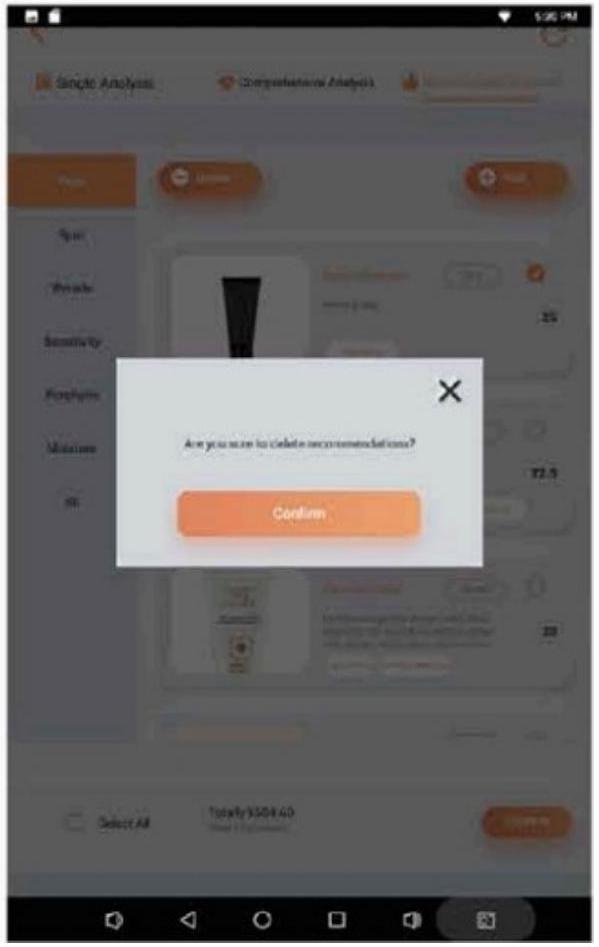
\includegraphics[alt={},max width=\textwidth]{018f02f8-3740-46eb-ab06-ecd68977d8ca-11_947_599_1635_3224}
\captionsetup{labelformat=empty}
\caption{Immagine 5-5-4}
\end{center}
\end{figure}

Aggiungi prodotti:Fai clic su "aggiungi" per inserire altri prodotti, come mostrato nella figura 5-5-3; Eliminare prodotti:Selezionare il prodotto da eliminare, cliccare su " Elimina " e confermare I' operazione, come mostrato nella figura 5-5-4;

\section{Gestione del negozio}
\subsection{Gestione dei file}
Dopo aver aggiunto con successo un cliente, il file del cliente appena creato è disponibile nella gestione del negozio, come mostrato nella figura 6-1-1. Seleziona un file cliente per visualizzare i dati dettagliati: nome, sesso, età, numero di telefono, data della rilevazione, data dell'ultimo test, tempo trascorso dalla rilevazione precedente e i 3 problemi cutanei più gravi (preoccupazioni). Barra di ricerca: Inserisci il nome del cliente o il numero di telefono per trovare rapidamente il file del cliente specificato.

Elenco clienti: Clicca per modificare l'ordine dell'elenco, come mostrato in

\begin{figure}[H]
\begin{center}
  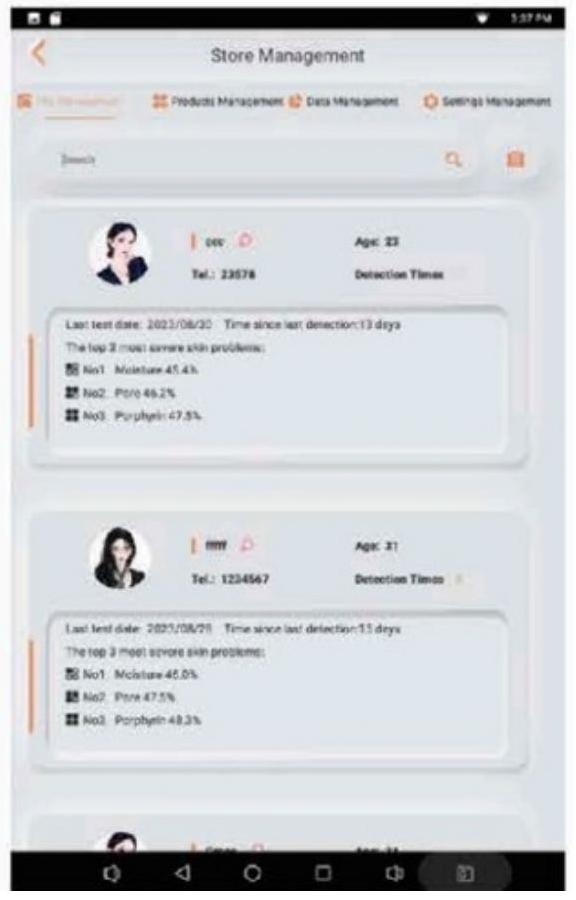
\includegraphics[alt={},max width=\textwidth]{018f02f8-3740-46eb-ab06-ecd68977d8ca-12_900_576_1295_449}
\captionsetup{labelformat=empty}
\caption{Immagine 6-1-1}
\end{center}
\end{figure}

Immagine 6-1-2.

\begin{figure}[H]
\begin{center}
  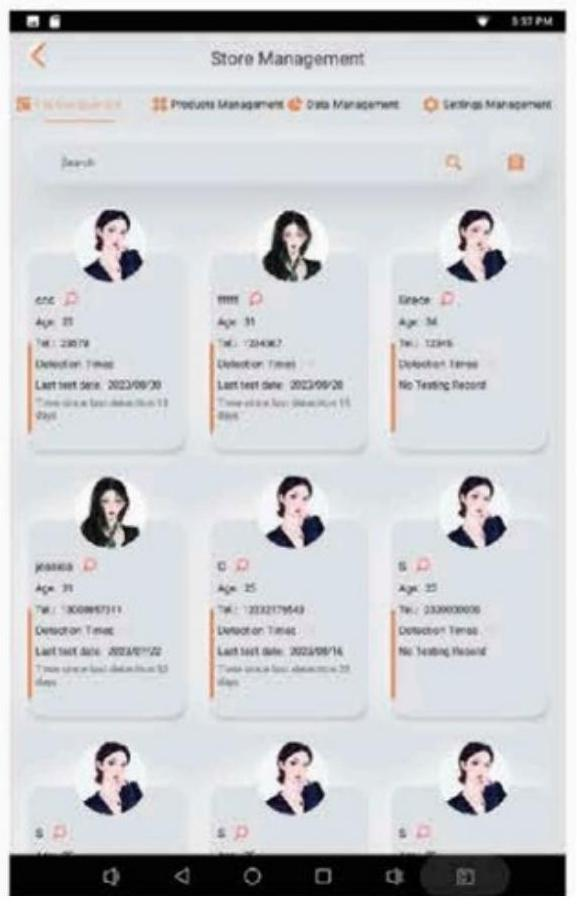
\includegraphics[alt={},max width=\textwidth]{018f02f8-3740-46eb-ab06-ecd68977d8ca-12_909_577_1292_1046}
\captionsetup{labelformat=empty}
\caption{Immagine 6-1-2}
\end{center}
\end{figure}

Modifica: come mostrato nella figura 6-1-3, clicca per modificare i dati del cliente Elimina il file del cliente: premi e teni premuto il file del cliente per cancellarlo, poi tocca su "conferma", come mostrato nella figura 6-1-4.\\
Fai clic sul file del cliente, come mostrato nella figura 6-1-5.

\begin{figure}[H]
\begin{center}
  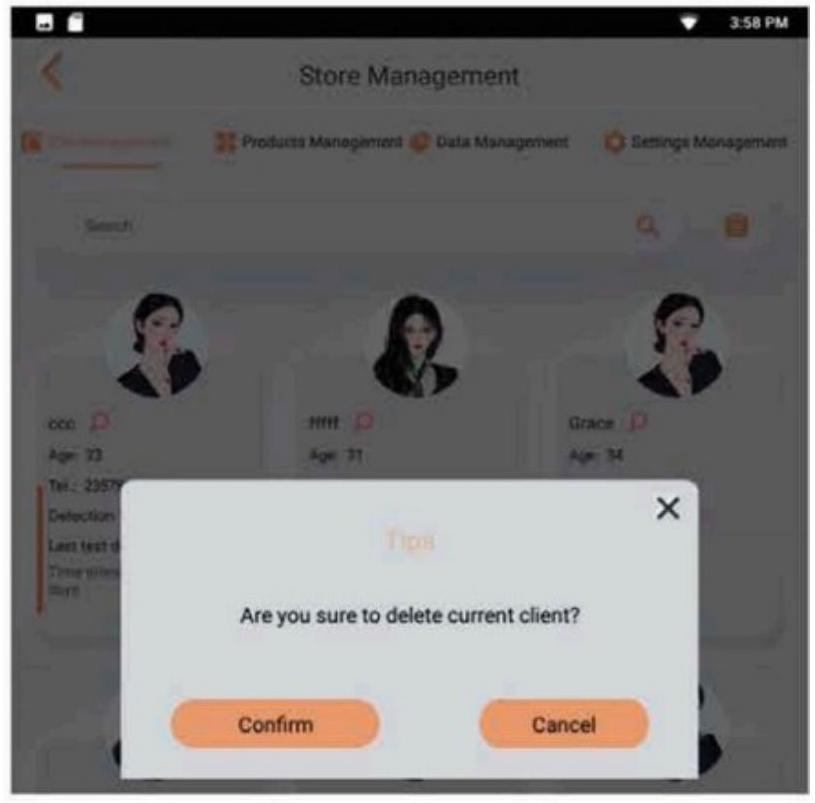
\includegraphics[alt={},max width=\textwidth]{018f02f8-3740-46eb-ab06-ecd68977d8ca-12_803_815_639_2378}
\captionsetup{labelformat=empty}
\caption{Immagine 6-1-4}
\end{center}
\end{figure}

\begin{figure}[H]
\begin{center}
  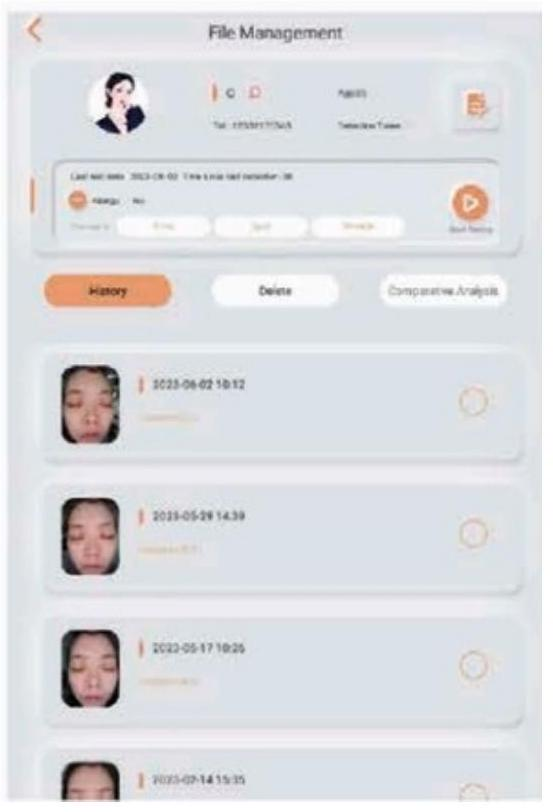
\includegraphics[alt={},max width=\textwidth]{018f02f8-3740-46eb-ab06-ecd68977d8ca-12_812_553_633_3302}
\captionsetup{labelformat=empty}
\caption{Immagine 6-1-5}
\end{center}
\end{figure}

Storia: contiene dati di rilevamento passati,\\
Cancellare: clicca $\_\_\_\_$ e "conferma" per eliminare l'elemento attualmente selezionato, oppure clicc □ per eliminare tutti i record del file, come mostrato nella figura 6-1-6

\begin{figure}[H]
\begin{center}
  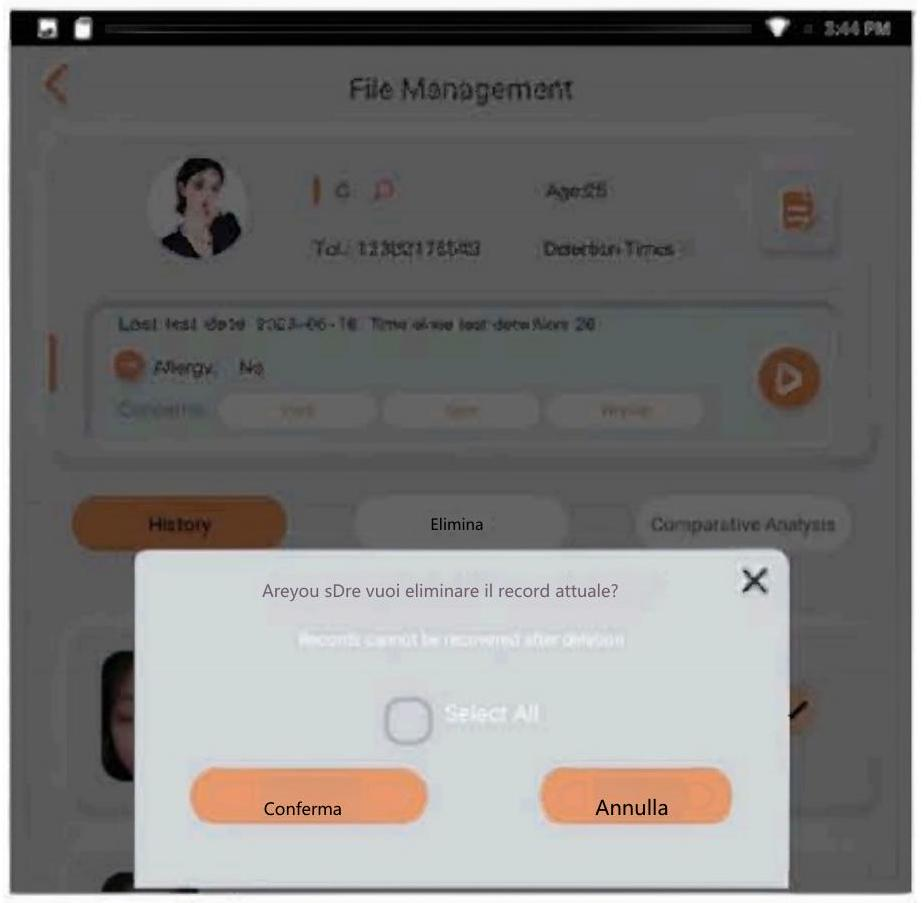
\includegraphics[alt={},max width=\textwidth]{018f02f8-3740-46eb-ab06-ecd68977d8ca-12_903_922_1670_2639}
\captionsetup{labelformat=empty}
\caption{Immagine 6-1-6}
\end{center}
\end{figure}

Analisi comparativa: seleziona i risultati del test relativi a due date diverse e fai clic su "Analisi comparativa" per visualizzare il rapporto, come mostrato nella figura 6-1-7. Le sei condizioni cutanee - Pore RGB, Spot RGB, Wrinkle RGB, Porphyrina UV e Umidità UV - possono essere ingrandite e confrontate una per una, come mostrato nella figura 6-1-8.

Clicca su "Confronta il rapporto"\\
Il cliente può visualizzare i risultati prima e dopo il test, come mostrato nella figura 6-1-9.

\begin{figure}[H]
\begin{center}
  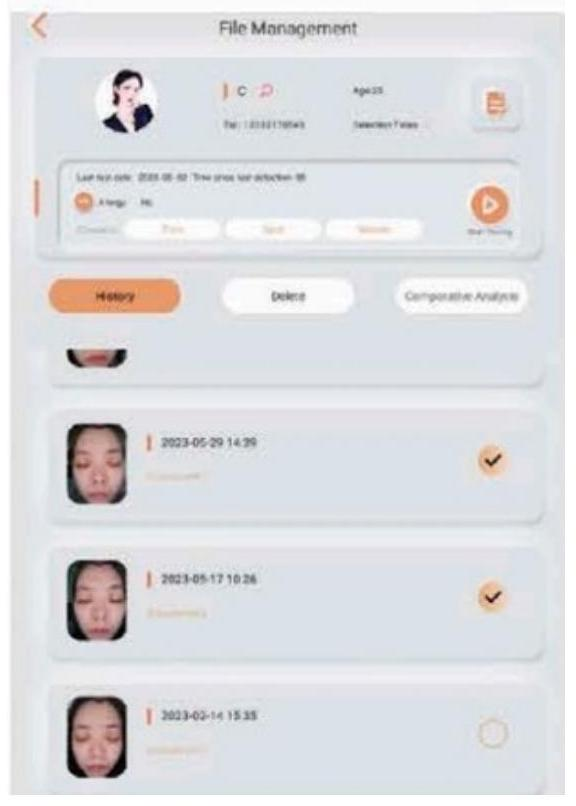
\includegraphics[alt={},max width=\textwidth]{018f02f8-3740-46eb-ab06-ecd68977d8ca-13_806_576_904_187}
\captionsetup{labelformat=empty}
\caption{Immagine 6-1-7}
\end{center}
\end{figure}

\begin{figure}[H]
\begin{center}
  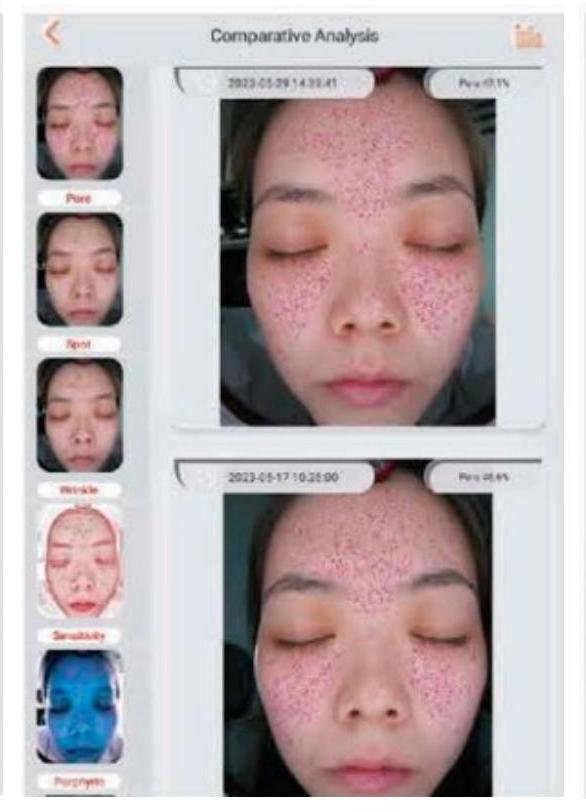
\includegraphics[alt={},max width=\textwidth]{018f02f8-3740-46eb-ab06-ecd68977d8ca-13_812_586_904_749}
\captionsetup{labelformat=empty}
\caption{Immagine 6-1-8}
\end{center}
\end{figure}

\begin{figure}[H]
\begin{center}
  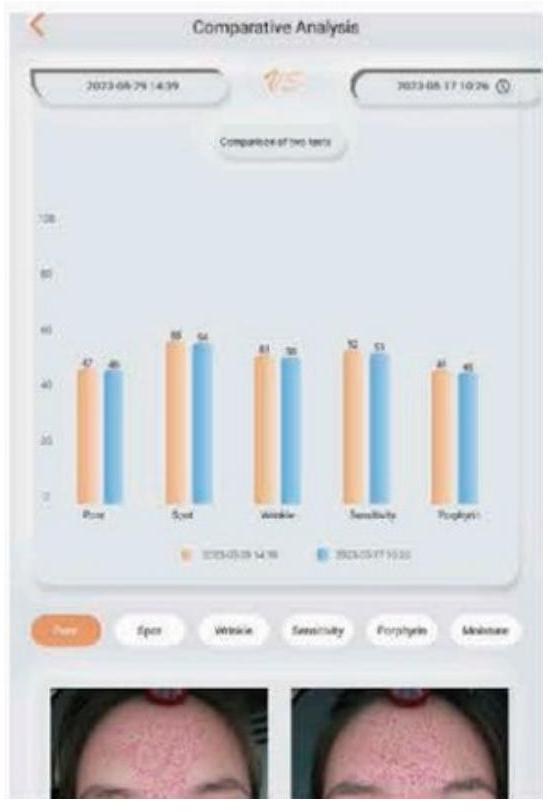
\includegraphics[alt={},max width=\textwidth]{018f02f8-3740-46eb-ab06-ecd68977d8ca-13_812_554_904_1324}
\captionsetup{labelformat=empty}
\caption{Immagine 6-1-9}
\end{center}
\end{figure}

\subsection{Gestione del prodotto}
Nella sezione gestione prodotto sono presenti 8 categorie di prodotti, come mostrato nella figura 6-2-1; è possibile scaricare in anticipo i prodotti tramite la funzione di informazioni di download presente nelle impostazioni (vedi 6.4.2 per maggiori dettagli). Visualizza i dettagli del prodotto: come mostrato nella figura 6-2-2, puoi controllare qui: nome del prodotto, istruzioni per l'uso, prezzo e problemi cutanei associati. Clicca su qualsiasi prodotto per visualizzarne i dettagli.\\
Eliminare il prodotto:Premere a lungo su qualsiasi prodotto, scegliendo di eliminare il prodotto attuale oppure selezionando più prodotti, come mostrato nella figura 6-2-

\begin{figure}[H]
\begin{center}
  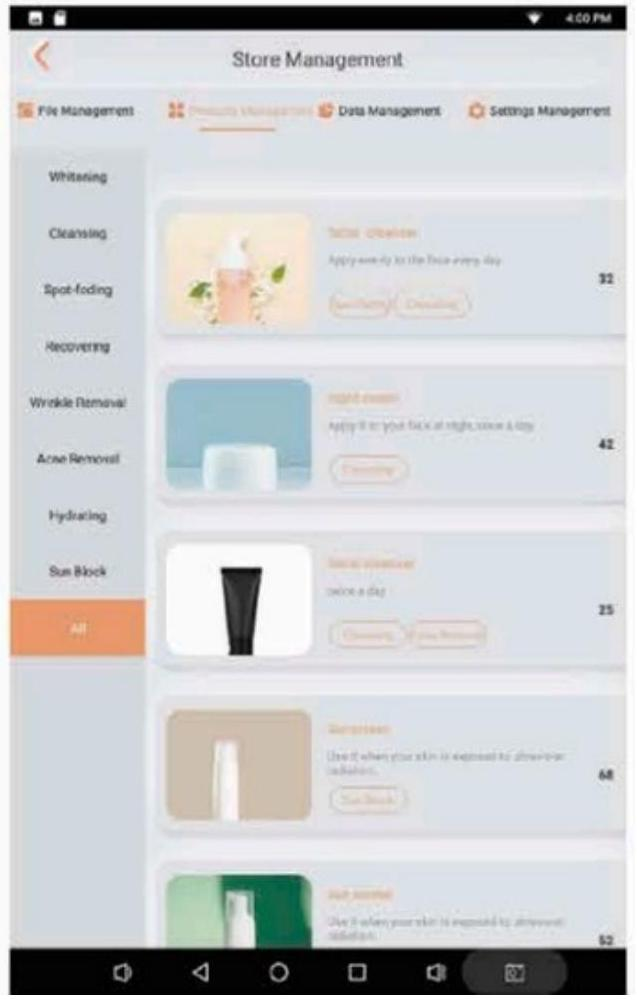
\includegraphics[alt={},max width=\textwidth]{018f02f8-3740-46eb-ab06-ecd68977d8ca-13_1006_637_213_2378}
\captionsetup{labelformat=empty}
\caption{Immagine 6-2-1}
\end{center}
\end{figure}

\begin{figure}[H]
\begin{center}
  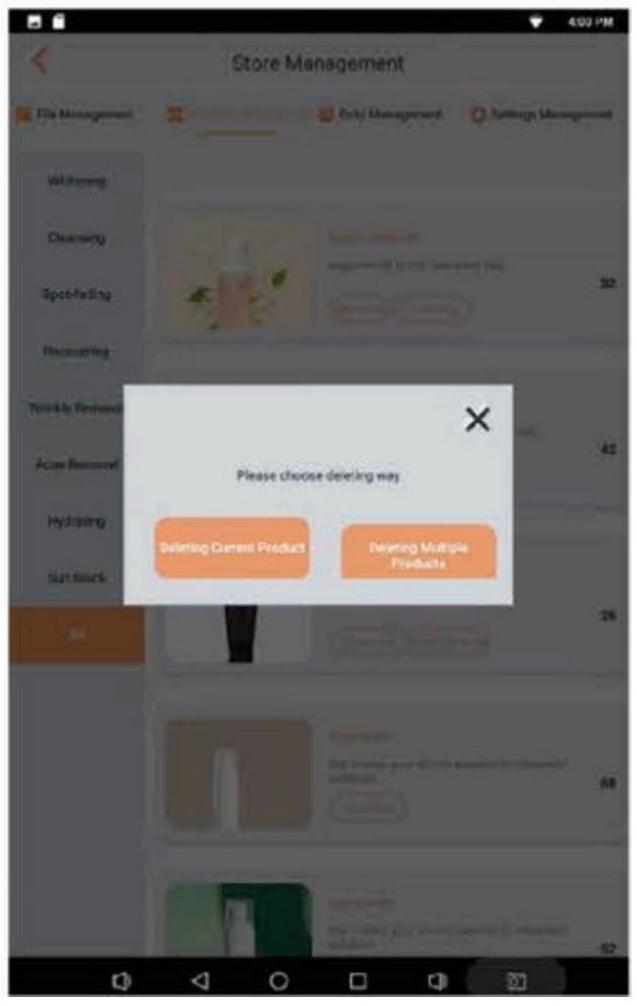
\includegraphics[alt={},max width=\textwidth]{018f02f8-3740-46eb-ab06-ecd68977d8ca-13_1006_637_1460_2365}
\captionsetup{labelformat=empty}
\caption{Immagine 6-2-3}
\end{center}
\end{figure}

\begin{figure}[H]
\begin{center}
  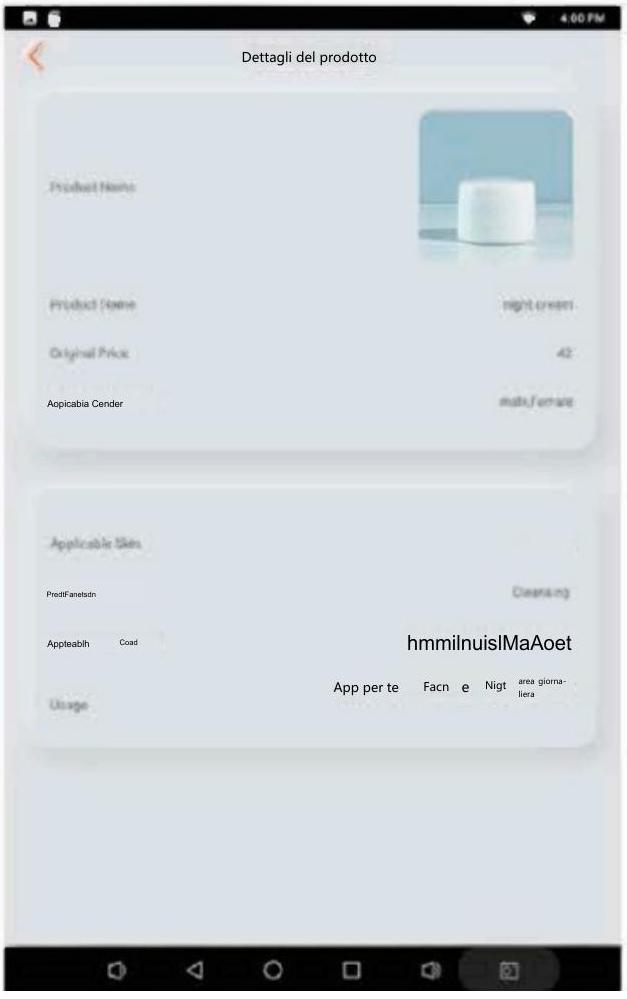
\includegraphics[alt={},max width=\textwidth]{018f02f8-3740-46eb-ab06-ecd68977d8ca-13_999_627_213_3102}
\captionsetup{labelformat=empty}
\caption{Immagine 6-2-2}
\end{center}
\end{figure}

\begin{figure}[H]
\begin{center}
  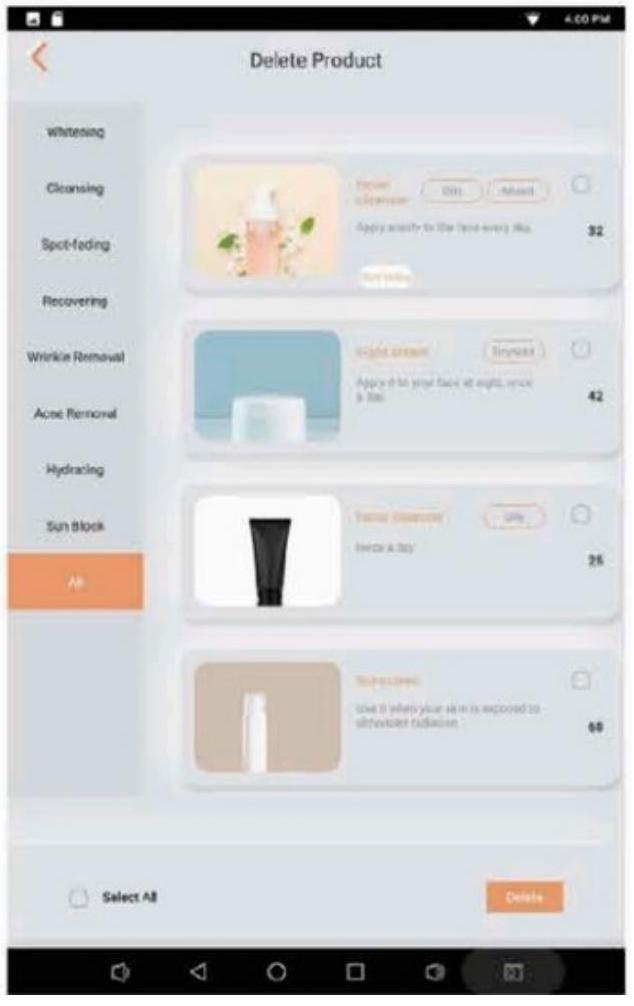
\includegraphics[alt={},max width=\textwidth]{018f02f8-3740-46eb-ab06-ecd68977d8ca-13_1006_634_1460_3095}
\captionsetup{labelformat=empty}
\caption{Immagine 6-2-4}
\end{center}
\end{figure}

36-2-4.

\subsection{Gestione dei dati}
Fai clic su "Interfaccia di gestione dati", dove puoi visualizzare le informazioni sulla percentuale relativa ai dati complessivi del cliente.\\
Innanzitutto, si nota che il numero totale di clienti rilevati è 15, come mostrato in

\begin{figure}[H]
\begin{center}
  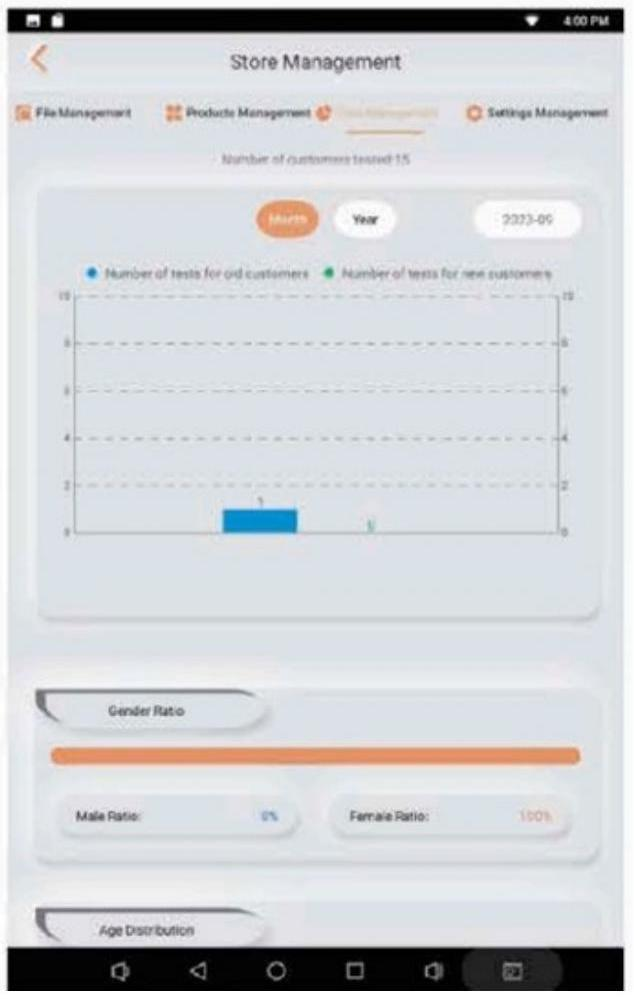
\includegraphics[alt={},max width=\textwidth]{018f02f8-3740-46eb-ab06-ecd68977d8ca-14_999_634_701_336}
\captionsetup{labelformat=empty}
\caption{Immagine 6-3-1}
\end{center}
\end{figure}

immagine 6-3-1 6-3-2.

\begin{figure}[H]
\begin{center}
  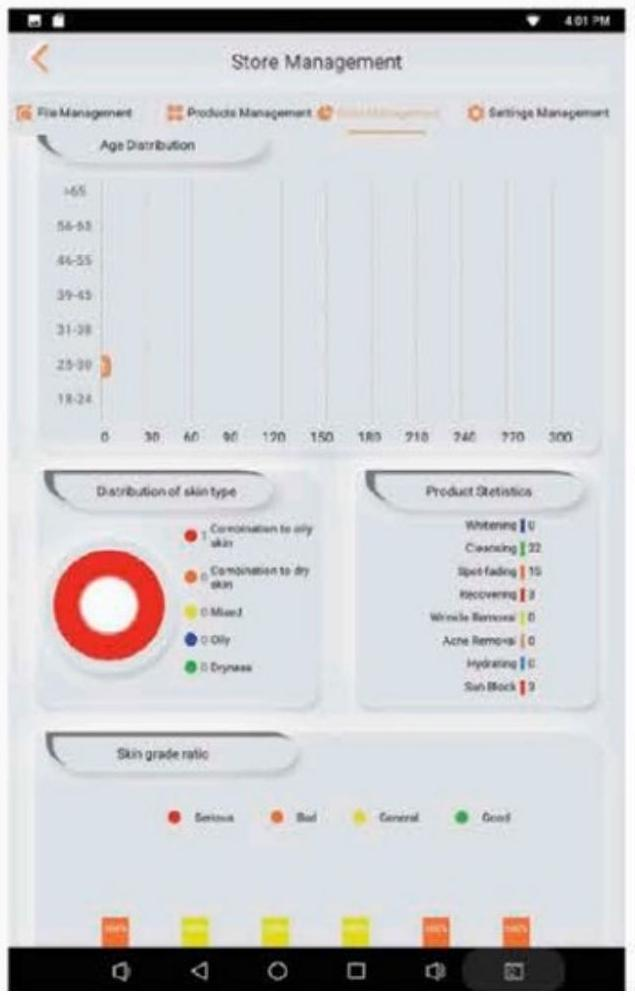
\includegraphics[alt={},max width=\textwidth]{018f02f8-3740-46eb-ab06-ecd68977d8ca-14_999_635_701_1059}
\captionsetup{labelformat=empty}
\caption{Immagine 6-3-2}
\end{center}
\end{figure}

Nella sezione "Statistiche dei dati di rilevamento", nei grafici "Anno" e "Mese" è possibile osservare il numero di ispezioni effettuate per clienti nuovi e esistenti. Ad esempio, nel settembre 2023, un solo cliente esistente è stato sottoposto a nuovo test, mentre non sono stati registrati test per nuovi clienti, come mostrato nella figura 6-3-1.\\
Nella sezione "rapporto di genere": tra i gruppi di clienti sottoposti a test nel settembre 2023, le donne rappresentano il 100\% del totale, come mostrato nella figura 6-3-1. Nella sezione "distribuzione per età": l'asse verticale indica l'intervallo di età dei clienti, mentre l'asse orizzontale indica l'intervallo di numero di clienti testati. Tra i gruppi di clienti testati nel settembre 2023, c'era 1 cliente nell' intervallo di età 25-30, come mostrato nella figura 6-3-2.

Nella sezione "Distribuzione dei tipi di pelle": Tra i gruppi di clienti testati a settembre 2023, l'attributo della pelle di un cliente è stato classificato come "combinato con pelle oleosa", come mostrato nella figura 6-3-2.\\
Nella sezione "Statistiche dei prodotti":Le categorie di prodotti raccomandate in totale in tutti i rapporti dei clienti di settembre 2023 includono: 22 prodotti per la pulizia, 15 prodotti per la rimozione delle macchie, 3 prodotti per la riparazione e 3 prodotti per la protezione solare, come mostrato nella figura 6-3-2.\\
Nella sezione "Skin grade ratio":ad esempio per quanto riguarda i pori, tra tutti i clienti testati, rispetto ai rispettivi coetanei, il $20 \%$ presenta un stato di pori "Generale", mentre l'80\% ha un stato di pori "Pessimo", come mostrato nella figura 6-3-3.

\begin{figure}[H]
\begin{center}
  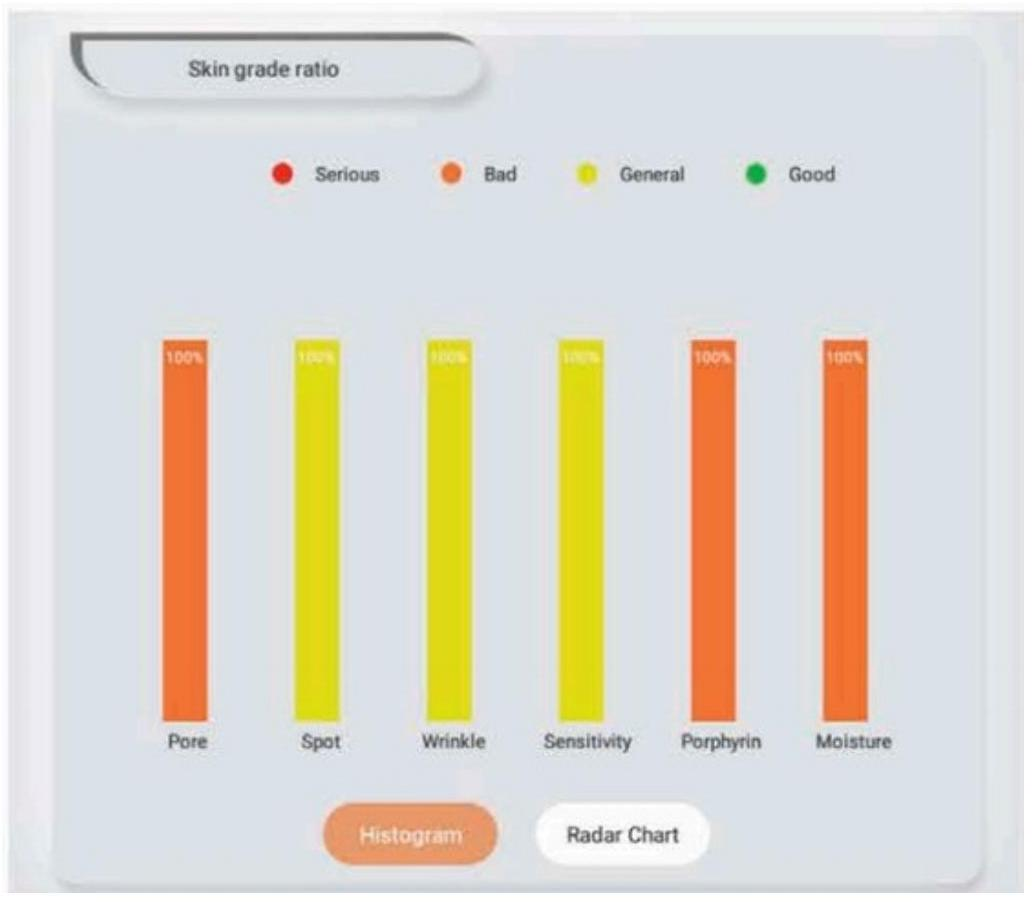
\includegraphics[alt={},max width=\textwidth]{018f02f8-3740-46eb-ab06-ecd68977d8ca-14_903_1032_1046_2584}
\captionsetup{labelformat=empty}
\caption{Immagine 6-3-3}
\end{center}
\end{figure}

\subsection{Gestione delle impostazioni}
\subsubsection{ID del terminale di legame}
Fai clic su "Gestione delle impostazioni", come mostrato nella figura 6-4-1.\\
Prima di tutto, richiedi un ID e una password in Cloud (vedi 7.3.1 per i dettagli), quindi fai clic su "Binding Terminal ID" per inserire ID e password, come mostrato nella figura 6-4-2.

\begin{figure}[H]
\begin{center}
  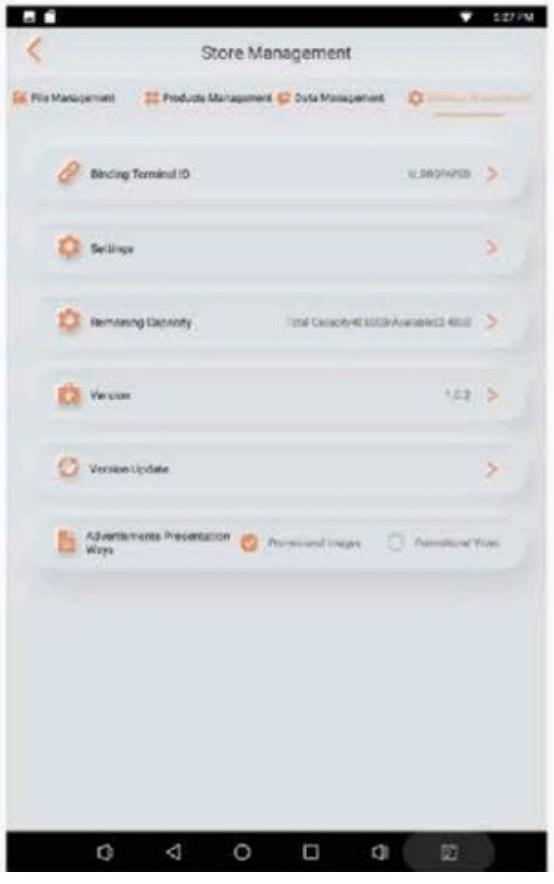
\includegraphics[alt={},max width=\textwidth]{018f02f8-3740-46eb-ab06-ecd68977d8ca-15_884_554_193_400}
\captionsetup{labelformat=empty}
\caption{Immagine 6-4-1}
\end{center}
\end{figure}

\begin{figure}[H]
\begin{center}
  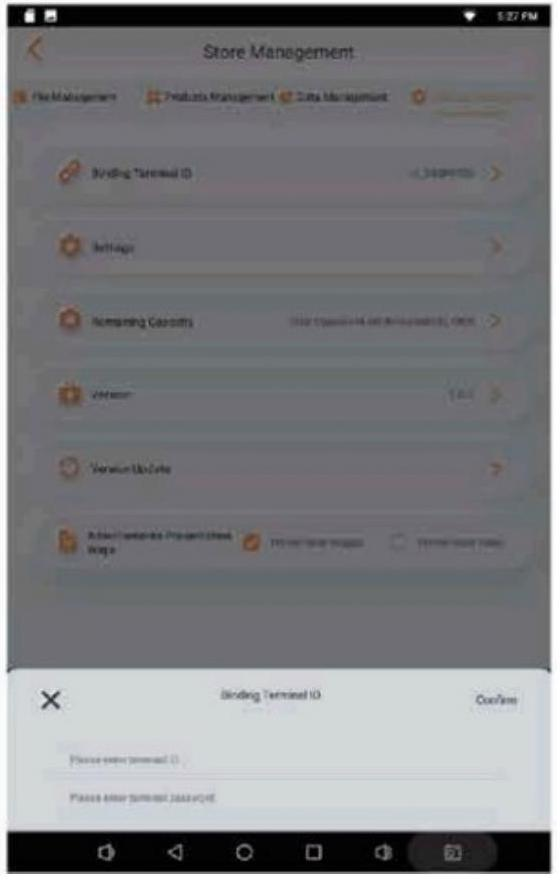
\includegraphics[alt={},max width=\textwidth]{018f02f8-3740-46eb-ab06-ecd68977d8ca-15_884_560_193_1063}
\captionsetup{labelformat=empty}
\caption{Immagine 6-4-2}
\end{center}
\end{figure}

\subsubsection{Impostazioni}
Fai clic su "Impostazioni", come mostrato nella figura 6-4-3.\\
Conessione Wi-Fi:Clicca su "Conessione Wi-Fi" per collegarti al Wi-Fi del negozio o a quello del dispositivo.Scarico delle informazioni:Prima di tutto, caricare sul cloud, in sequenza, il logo e la pubblicità del negozio (vedi 7.3.2 per i dettagli), il prodotto (vedi 7.2.3 per i dettagli) e le suggerimenti di condizionamento (vedi 7.3.4 per i dettagli) sul sito web del cloud.\\
Successivamente utilizza l'"ID del terminale" per connettersi al cloud e al software di analisi (vedi 7.3.1 per i dettagli).\\
Infine, clicca su "LOGO Download", "Advertisement Download", "Product Download" e "Conditioning Suggestion Download" uno dopo l'altro, selezionando il contenuto corrispondente da scaricare e salvare.\\
Backup e ripristino:Fai clic su "Backup" per salvare tutti i dati presenti nel software di analisi. Fai clic su "Ripristino" per recuperare tutti i dati presenti nel software di analisi.\\
Si prega di connettersi alla rete Wi-Fi per attivare il dispositivo:Se il dispositivo non riesce a scattare foto, cliccate qui per attivarlo oppure contattate l'amministratore per risolvere il problema.\\
Invito al marchio: Dopo aver richiesto un codice di invito al marchio nel cloud (vedi 7.2.2 per i dettagli), apri l'opzione "Invito al marchio" nel software di analisi, come mostrato nella figura 6-4-3. A quel punto, fai clic per scaricare i prodotti. Per scaricare i prodotti dello stesso marchio in un'unica volta, devi inserire il codice di invito al marchio, come mostrato nella figura 6-4-4.

\begin{figure}[H]
\begin{center}
  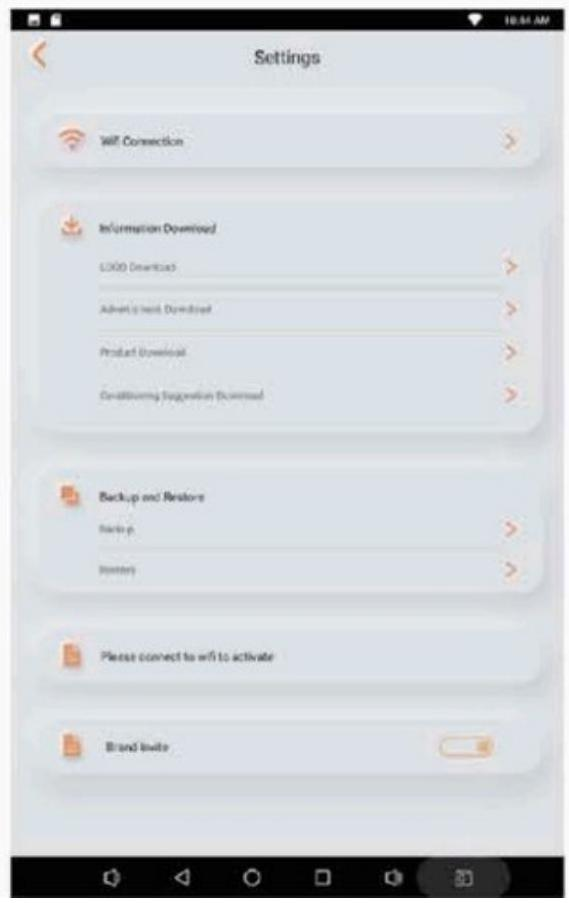
\includegraphics[alt={},max width=\textwidth]{018f02f8-3740-46eb-ab06-ecd68977d8ca-15_903_569_206_2462}
\captionsetup{labelformat=empty}
\caption{Immagine 6-4-3}
\end{center}
\end{figure}

\begin{figure}[H]
\begin{center}
  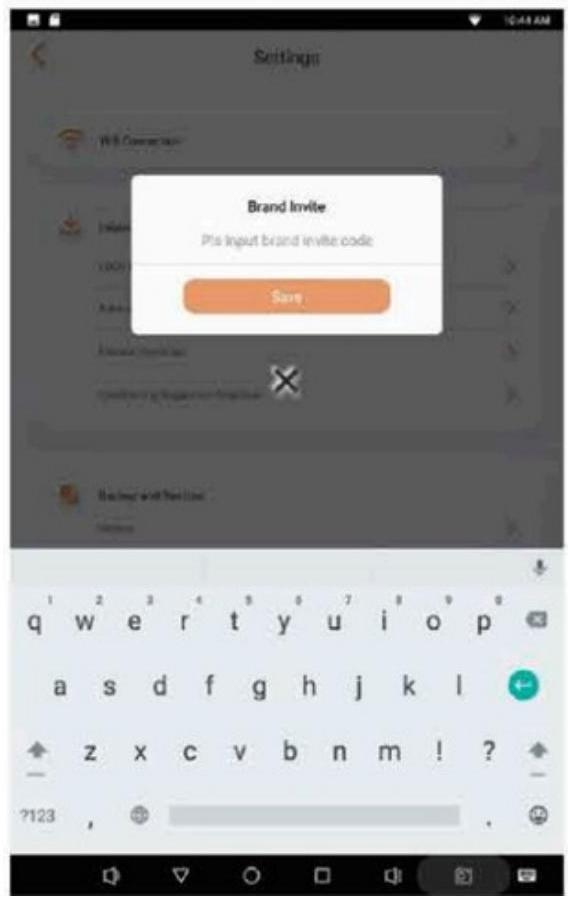
\includegraphics[alt={},max width=\textwidth]{018f02f8-3740-46eb-ab06-ecd68977d8ca-15_900_573_206_3160}
\captionsetup{labelformat=empty}
\caption{Immagine 6-4-4}
\end{center}
\end{figure}

\subsubsection{Capacità residua}
Quello che appare qui è la capacità di MX , come mostrato nella figura 6-4-1.

\subsubsection{Versione}
Quello che appare qui è il numero di versione del sistema di analisi attuale, come mostrato nella figura 6-4-1.

\subsubsection{Aggiornamento della versione}
Fai clic su "Version Update" per ottenere l'ultima versione del sistema, come mostrato nella figura 6-4-1.

\subsubsection{Presentazione degli annunci in diversi modi}
Fai clic sull'app del sistema di analisi per accedere all'interfaccia pubblicitaria, dove puoi inserire immagini o video promozionali. Non c'è limite al numero di immagini da caricare e puoi caricare un solo video, come mostrato nella figura 6-4-1.

\section{Cloud}
\section{Cerca sul sito web:https://emx.milisun.com/}
accedi alla figura 5-1 e registra un account. Come mostrato nelle figure 7-1-1 e 7-1-2.

\begin{figure}[H]
\begin{center}
  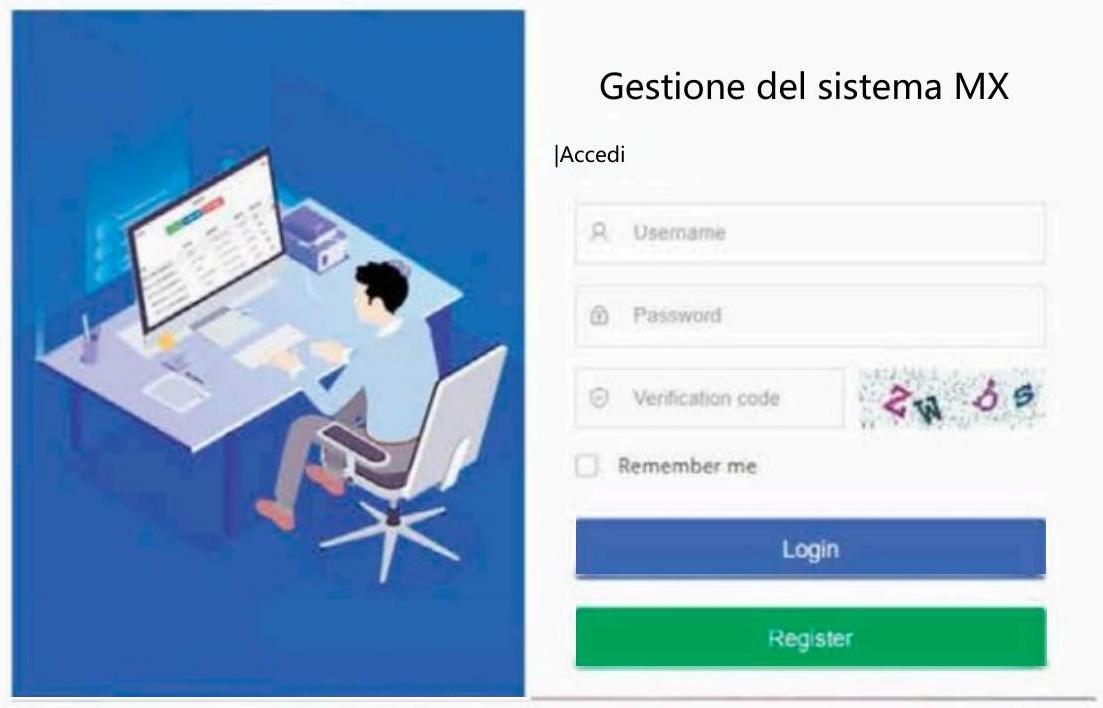
\includegraphics[alt={},max width=\textwidth]{018f02f8-3740-46eb-ab06-ecd68977d8ca-16_708_1103_575_394}
\captionsetup{labelformat=empty}
\caption{Immagine 7-1-1}
\end{center}
\end{figure}

\begin{figure}[H]
\begin{center}
  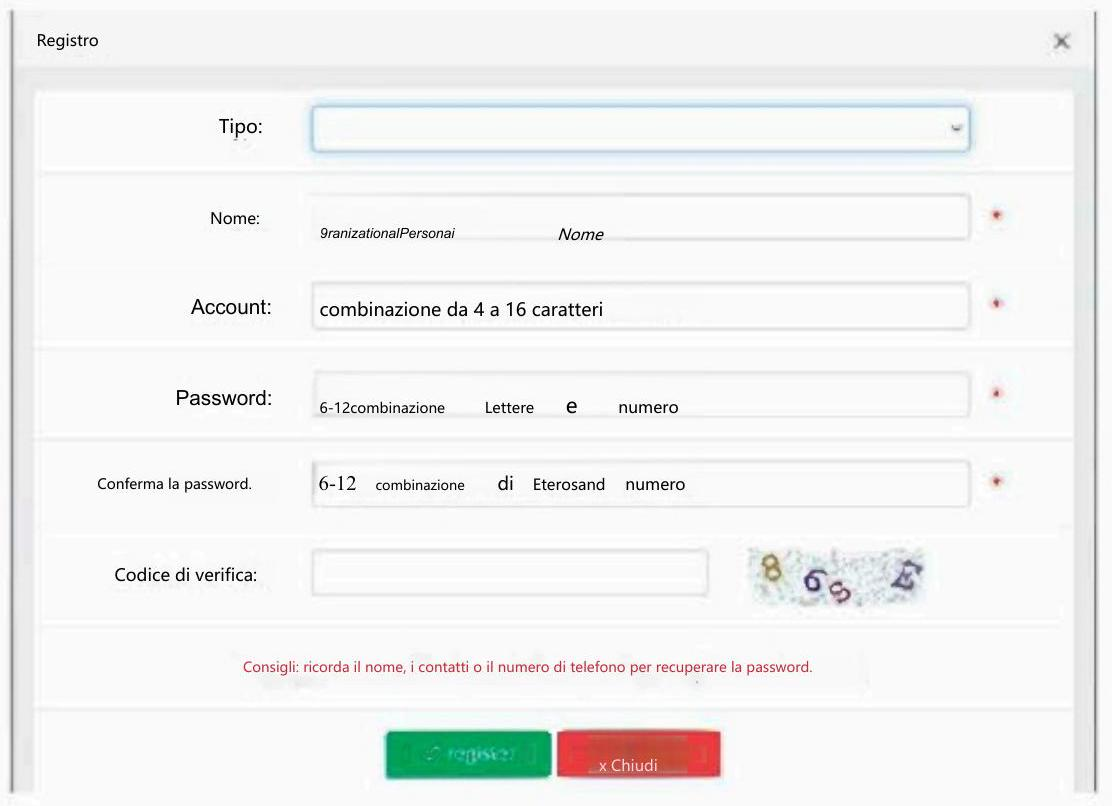
\includegraphics[alt={},max width=\textwidth]{018f02f8-3740-46eb-ab06-ecd68977d8ca-16_806_1112_1450_368}
\captionsetup{labelformat=empty}
\caption{Immagine 7-1-2}
\end{center}
\end{figure}

\subsection{Gestione del sistema}
\subsubsection{Organizzazione}
Fai clic su 'Organizzazione' per accedere alla figura 7-1-3. Qui puoi verificare le informazioni dell'account cloud e gestire anche gli account secondari.

\begin{figure}[H]
\begin{center}
  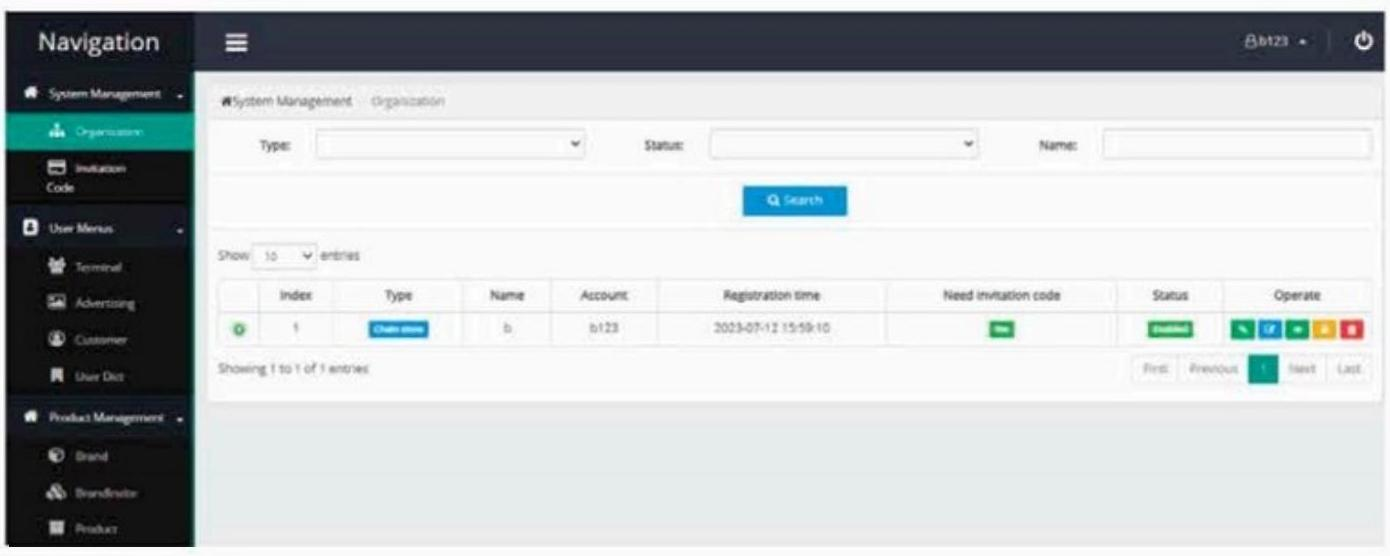
\includegraphics[alt={},max width=\textwidth]{018f02f8-3740-46eb-ab06-ecd68977d8ca-16_556_1390_701_2404}
\captionsetup{labelformat=empty}
\caption{Immagine 7-1-3}
\end{center}
\end{figure}

\subsubsection{Codice di invito}
Fai clic su "Invitation Code" per aggiungere un codice di invito, come mostrato nell'immagine 7-1-47-1-5. Registra un sottoconto (c) della cloud (ad esempio, come nell'immagine 7-1-2, seleziona "beauty salon o personal"). Inserisci il codice di invito dell'account della catena nel campo "Organizzazione - Collegare" del sottoconto, come mostrato nell'immagine 7-1-6.

Le catene di negozi possono condividere prodotti, annunci, ultime notizie e casi di successo con i sottocanali tramite un codice di invito.

\begin{figure}[H]
\begin{center}
  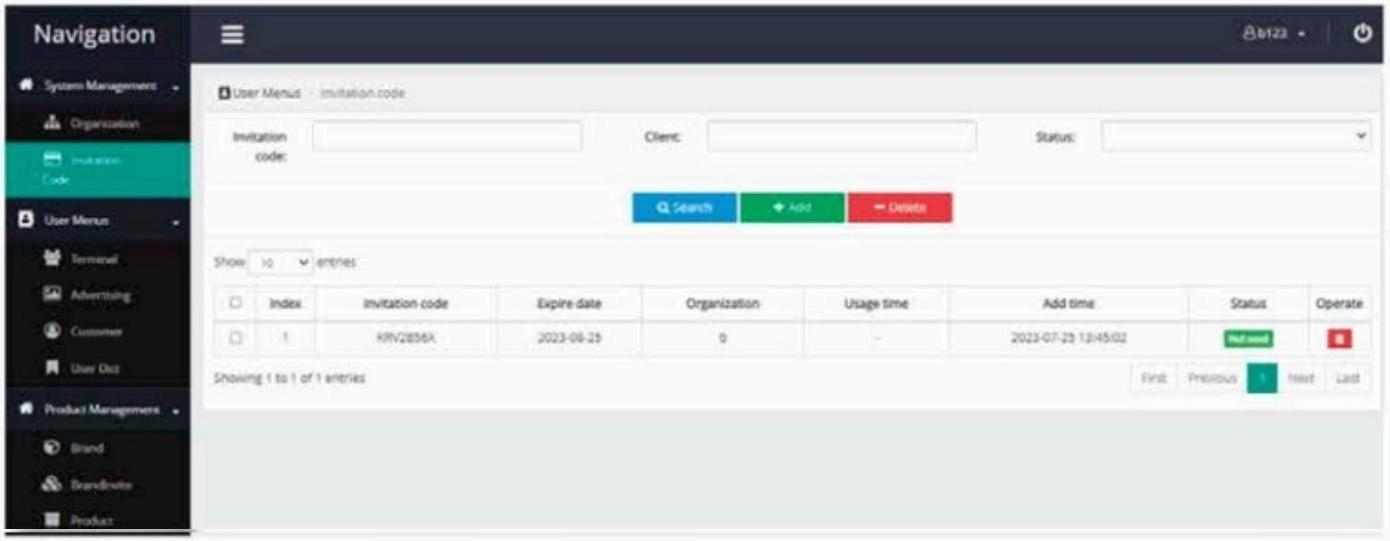
\includegraphics[alt={},max width=\textwidth]{018f02f8-3740-46eb-ab06-ecd68977d8ca-16_541_1390_2119_2407}
\captionsetup{labelformat=empty}
\caption{Immagine 7-1-4}
\end{center}
\end{figure}

\footnotetext{Nota: sono disponibili tre tipi di account: negozio a catena, salone di bellezza e persona fisica. Si prega di selezionare il tipo più adatto durante la registrazione. Il negozio a catena può gestire sia saloni di bellezza che persone fisiche, mentre il salone di bellezza può Gestione del conto personale.
}\begin{figure}[H]
\begin{center}
  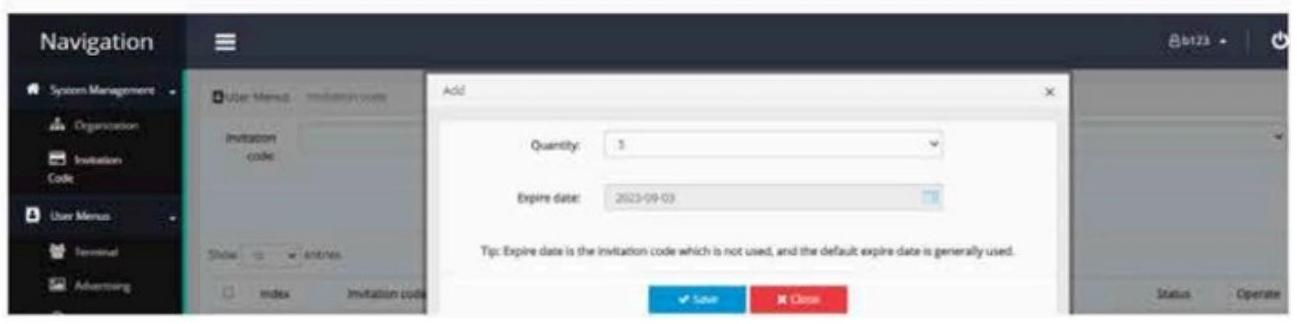
\includegraphics[alt={},max width=\textwidth]{018f02f8-3740-46eb-ab06-ecd68977d8ca-17_324_1297_197_387}
\captionsetup{labelformat=empty}
\caption{Immagine 7-1-5}
\end{center}
\end{figure}

\begin{table}[h]
\begin{center}
\begin{tabular}{|l|l|}
\hline
Navigazione & Bc 12 • \\
\hline
 &  \\
\hline
 &  \\
\hline
\multirow{3}{*}{} &  \\
\hline
 & Cperase \\
\hline
 &  \\
\hline
\end{tabular}
\captionsetup{labelformat=empty}
\caption{Immagine 7-1-6}
\end{center}
\end{table}

\subsection{Gestione del prodotto}
\subsubsection{Brand}
Fai clic su "Brand" per aggiungere un marchio di prodotto, come mostrato nelle figure 7-2-1 e 7-2-2.\\
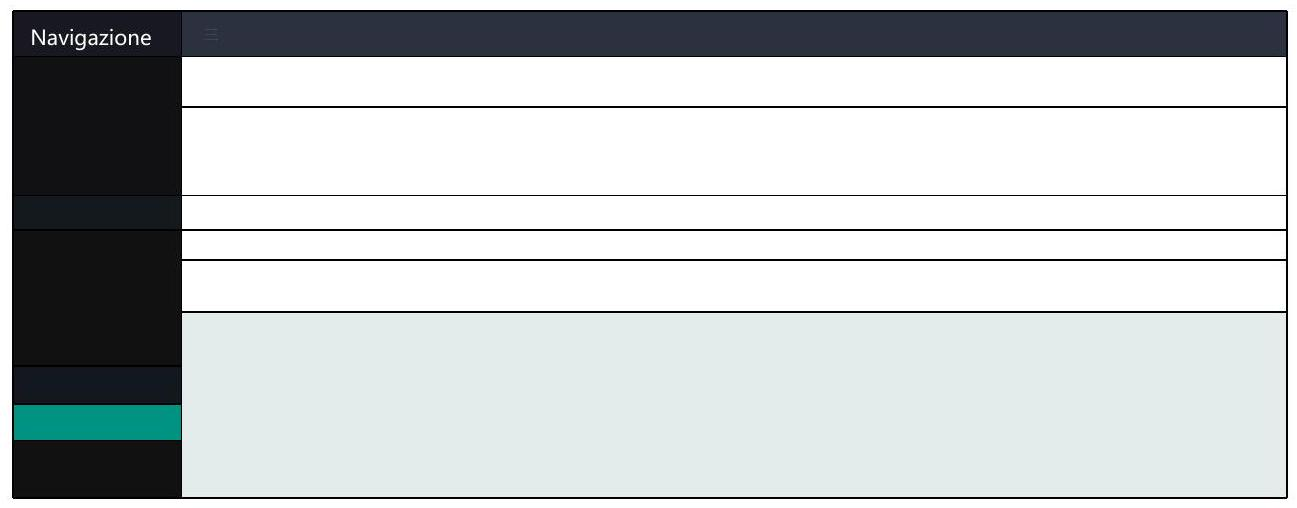
\includegraphics[max width=\textwidth, alt={}, center]{018f02f8-3740-46eb-ab06-ecd68977d8ca-17_508_1297_1460_329}

\begin{figure}[H]
\begin{center}
  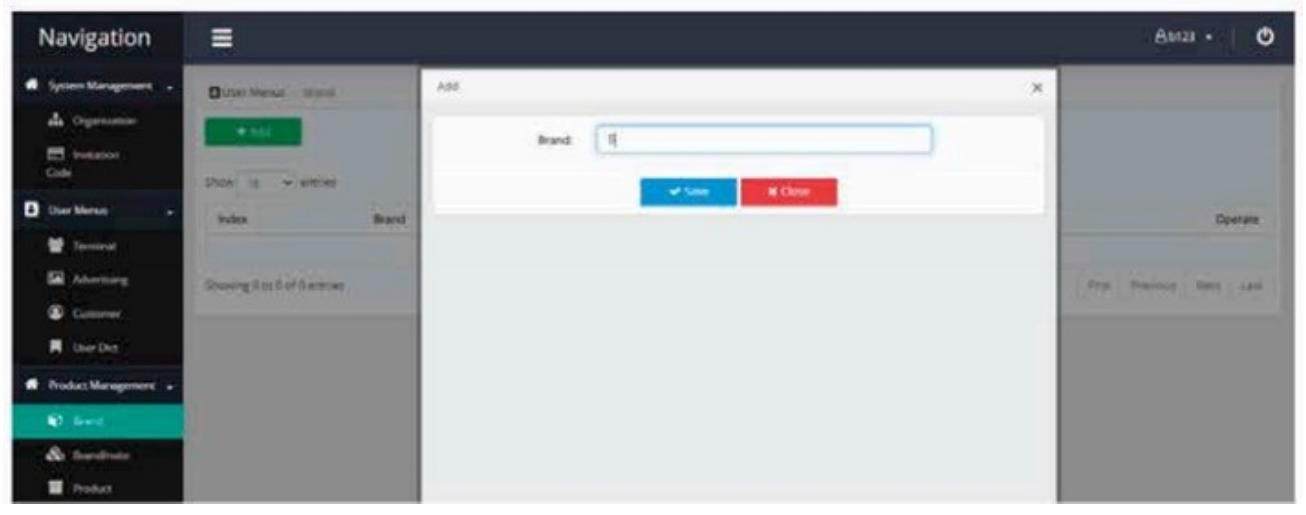
\includegraphics[alt={},max width=\textwidth]{018f02f8-3740-46eb-ab06-ecd68977d8ca-17_515_1306_2080_352}
\captionsetup{labelformat=empty}
\caption{Immagine 7-2-2}
\end{center}
\end{figure}

\subsubsection{BrandInvite}
Clicca su "Brandlnvite" per aggiungere un InvitoCodice e puoi scaricare prodotti della stessa marca in lotti contemporaneamente utilizzando il codice di invito \href{http://brandinvite.as}{brandinvite.as} mostrato nella figura 7-2-37-2-47-2-5.\\
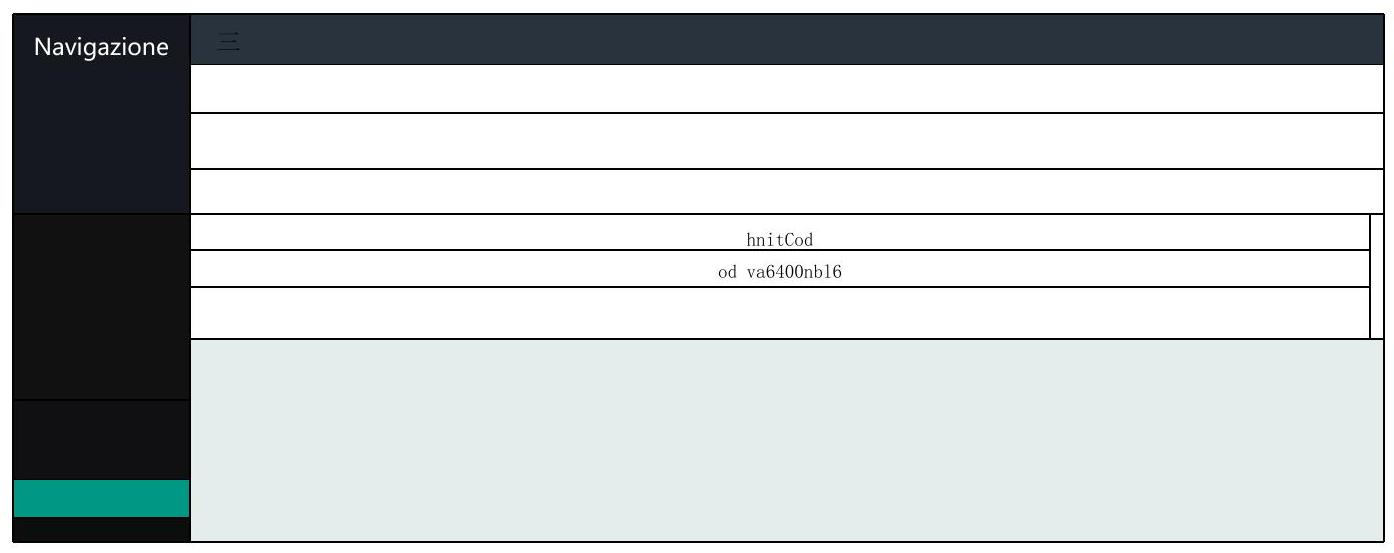
\includegraphics[max width=\textwidth, alt={}, center]{018f02f8-3740-46eb-ab06-ecd68977d8ca-17_553_1394_620_2397}

\begin{figure}[H]
\begin{center}
  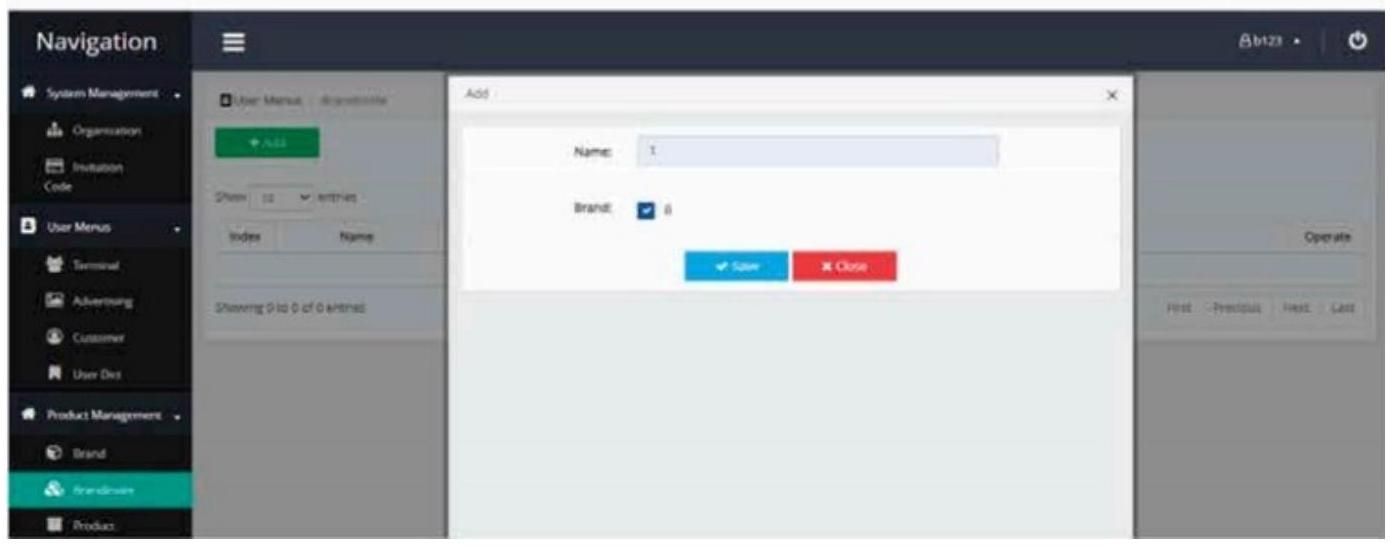
\includegraphics[alt={},max width=\textwidth]{018f02f8-3740-46eb-ab06-ecd68977d8ca-17_547_1390_1273_2381}
\captionsetup{labelformat=empty}
\caption{Immagine 7-2-4}
\end{center}
\end{figure}

Navigazione

\subsubsection{Prodotto}
Fai clic su "Product" e su "Add" per caricare prodotti di bellezza, come mostrato nella figura 7-2-6.

Ghiaccio •

\section{Immagine 7-2-6}
Compila le informazioni relative a "attributi del prodotto" e "problema della skin applicativa", come nome del prodotto, prezzo, genere di applicazione, skin applicativa, attributi del prodotto, pubblico di destinazione, modalità d' uso e immagine del prodotto, come mostrato nelle figure 7-2-7 e 7-2-8.

\begin{figure}[H]
\begin{center}
  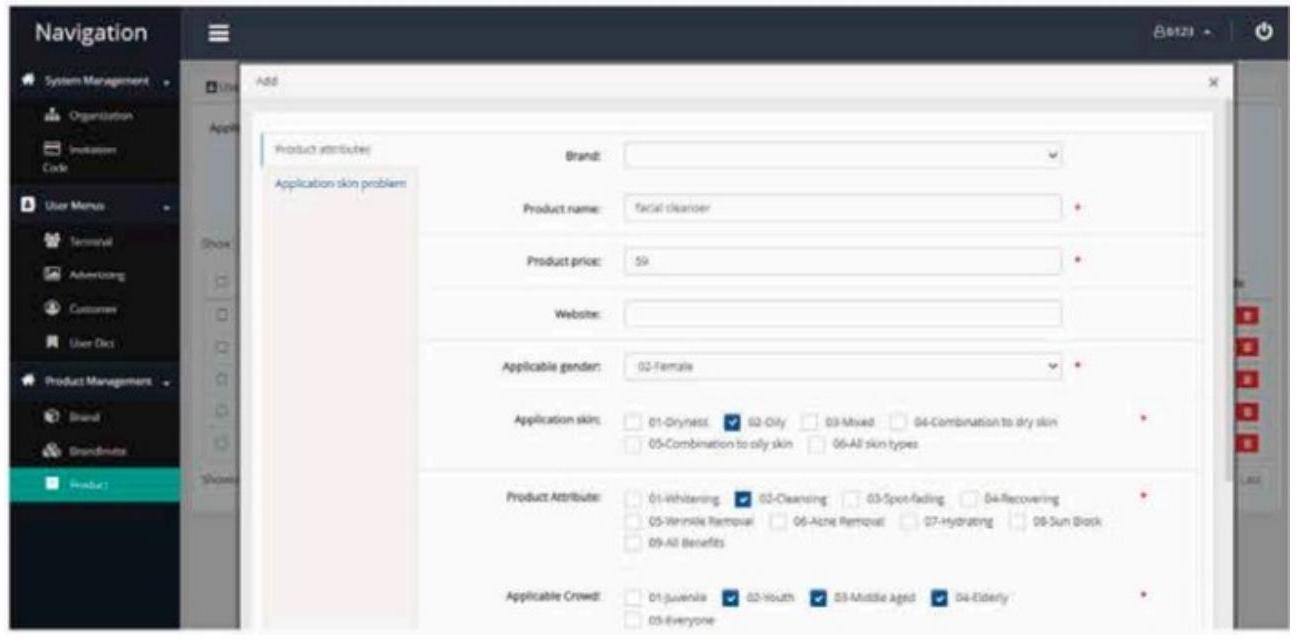
\includegraphics[alt={},max width=\textwidth]{018f02f8-3740-46eb-ab06-ecd68977d8ca-18_641_1297_1360_355}
\captionsetup{labelformat=empty}
\caption{Immagine 7-2-7(A)}
\end{center}
\end{figure}

\begin{figure}[H]
\begin{center}
  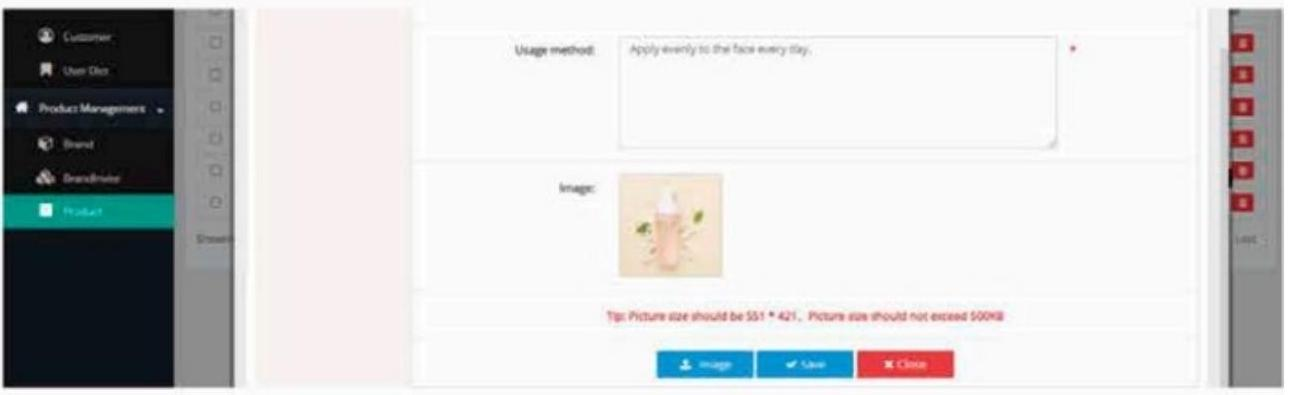
\includegraphics[alt={},max width=\textwidth]{018f02f8-3740-46eb-ab06-ecd68977d8ca-18_395_1291_2181_361}
\captionsetup{labelformat=empty}
\caption{Immagine 7-2-7(B)}
\end{center}
\end{figure}

\begin{figure}[H]
\begin{center}
  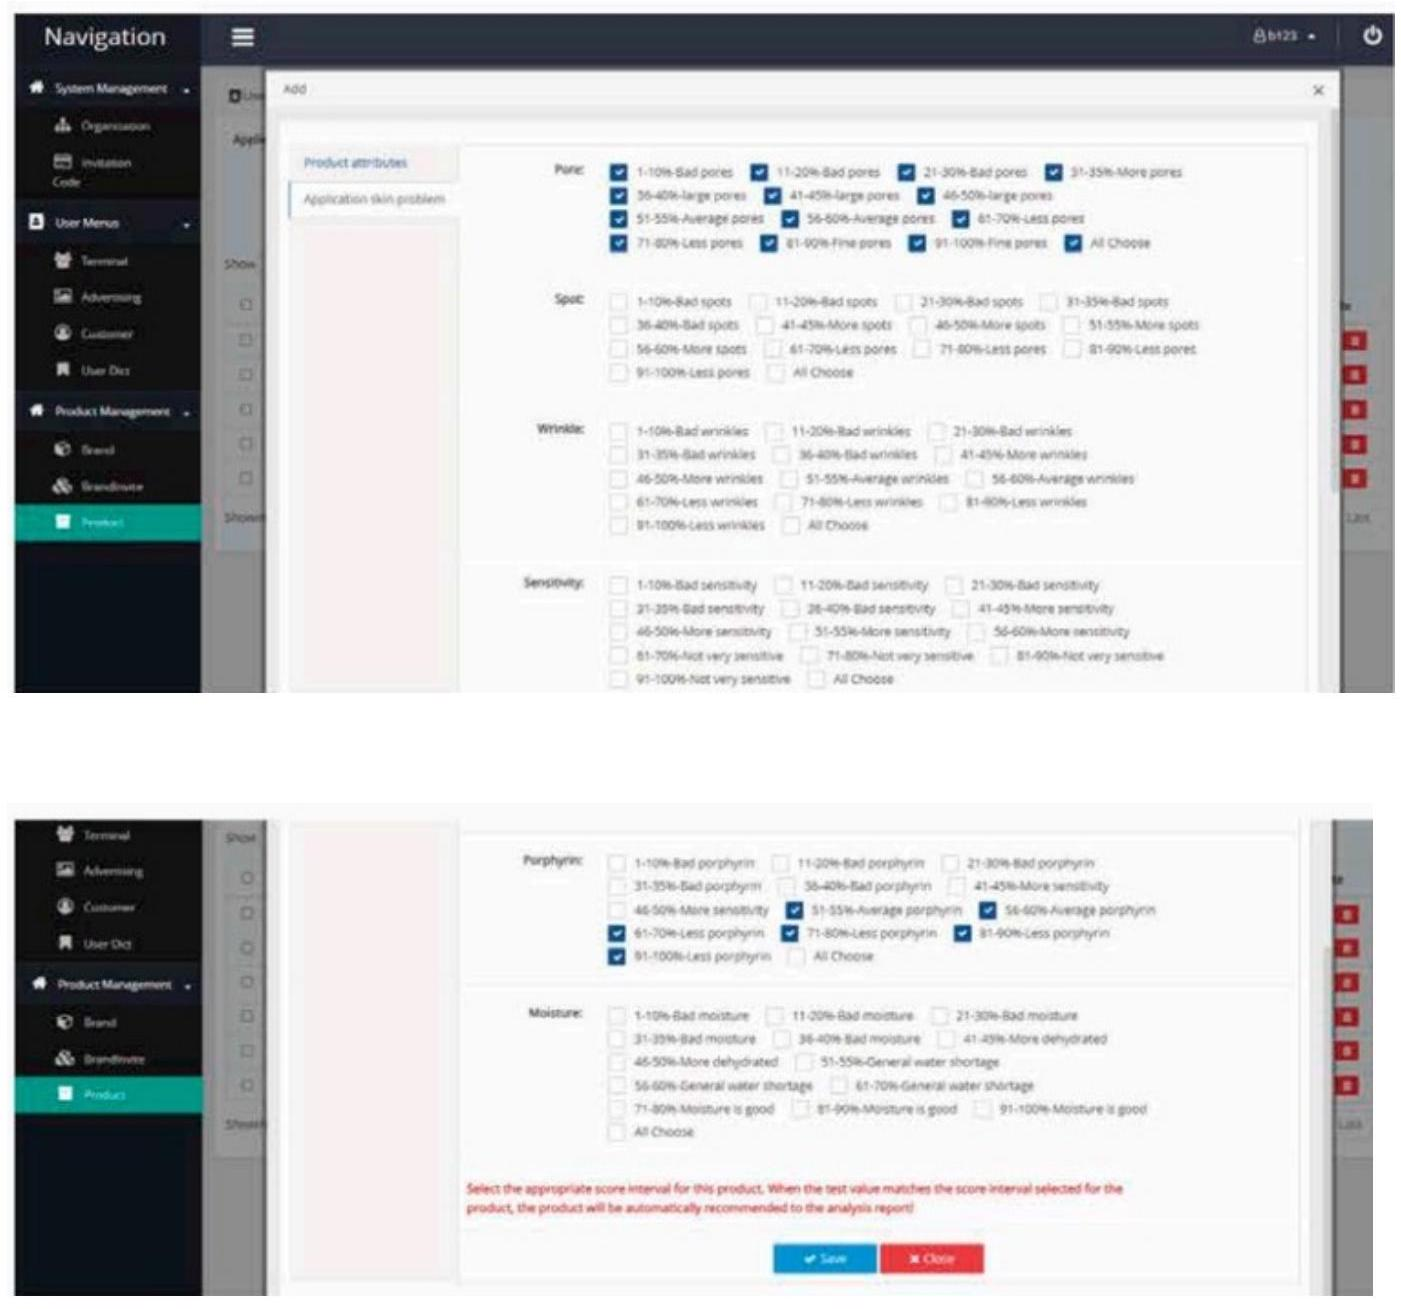
\includegraphics[alt={},max width=\textwidth]{018f02f8-3740-46eb-ab06-ecd68977d8ca-18_1309_1401_197_2416}
\captionsetup{labelformat=empty}
\caption{Immagine 7-2-8}
\end{center}
\end{figure}

\subsection{Menù utente}
\subsubsection{Terminal}
Fai clic su "Terminal" e su "Aggiungi" per generare l'ID del terminale e la password, come mostrato nella figura 7-3-17-3-27-3-3.

\begin{figure}[H]
\begin{center}
  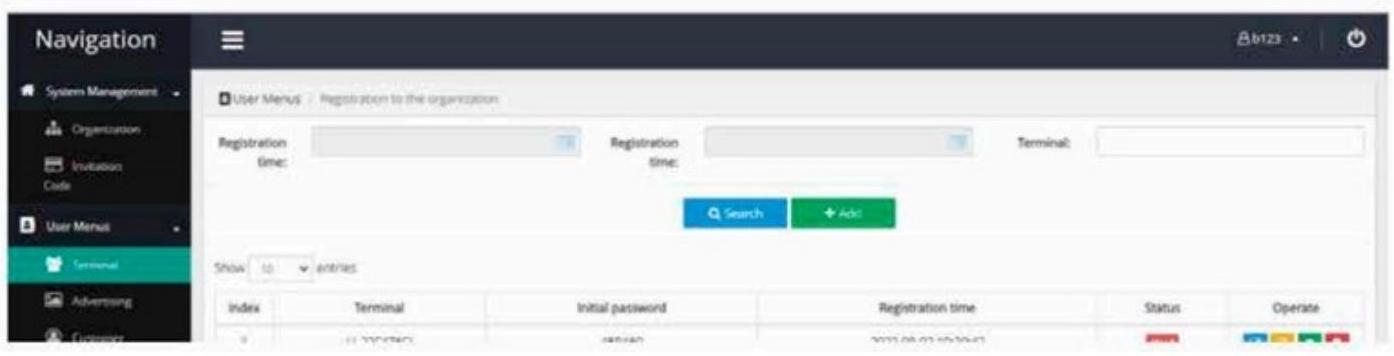
\includegraphics[alt={},max width=\textwidth]{018f02f8-3740-46eb-ab06-ecd68977d8ca-18_356_1394_2171_2423}
\captionsetup{labelformat=empty}
\caption{Immagine 7-3-1}
\end{center}
\end{figure}

\begin{figure}[H]
\begin{center}
  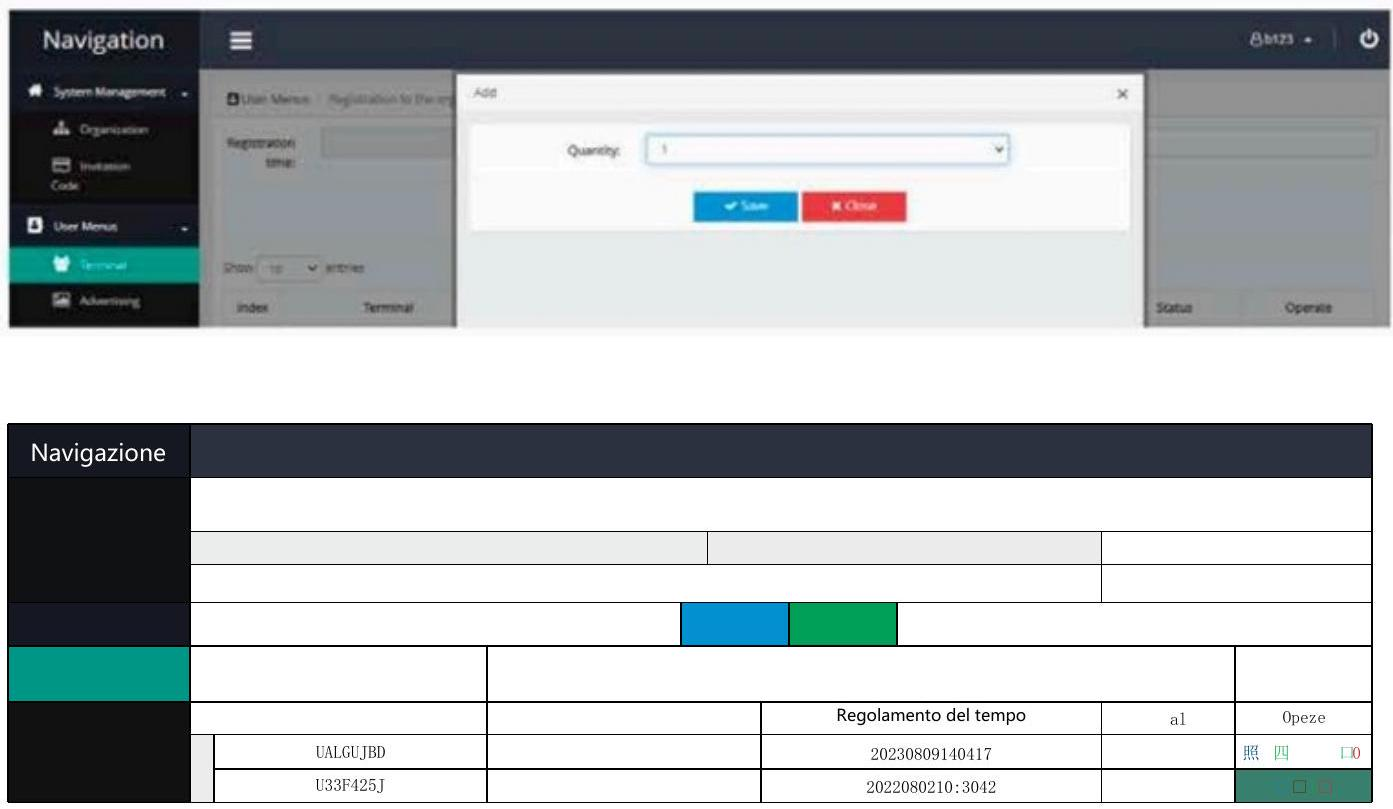
\includegraphics[alt={},max width=\textwidth]{018f02f8-3740-46eb-ab06-ecd68977d8ca-19_809_1393_193_336}
\captionsetup{labelformat=empty}
\caption{Immagine 7-3-3}
\end{center}
\end{figure}

\subsubsection{Pubblicità/Logo}
Fai clic su "Annuncio", come mostrato nella figura 7-3-4. Fai clic su "Naviga" per aggiungere un'immagine pubblicitaria o un'immagine del logo. Presta attenzione alle dimensioni delle immagini, come mostrato nella figura 7-3-5.

\begin{figure}[H]
\begin{center}
  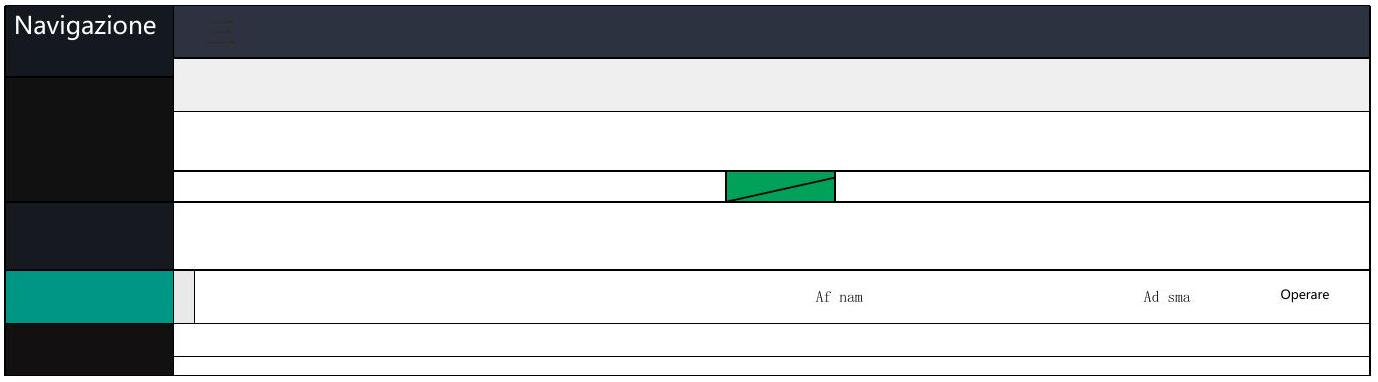
\includegraphics[alt={},max width=\textwidth]{018f02f8-3740-46eb-ab06-ecd68977d8ca-19_382_1378_1431_316}
\captionsetup{labelformat=empty}
\caption{Immagine 7-3-4}
\end{center}
\end{figure}

\begin{figure}[H]
\begin{center}
  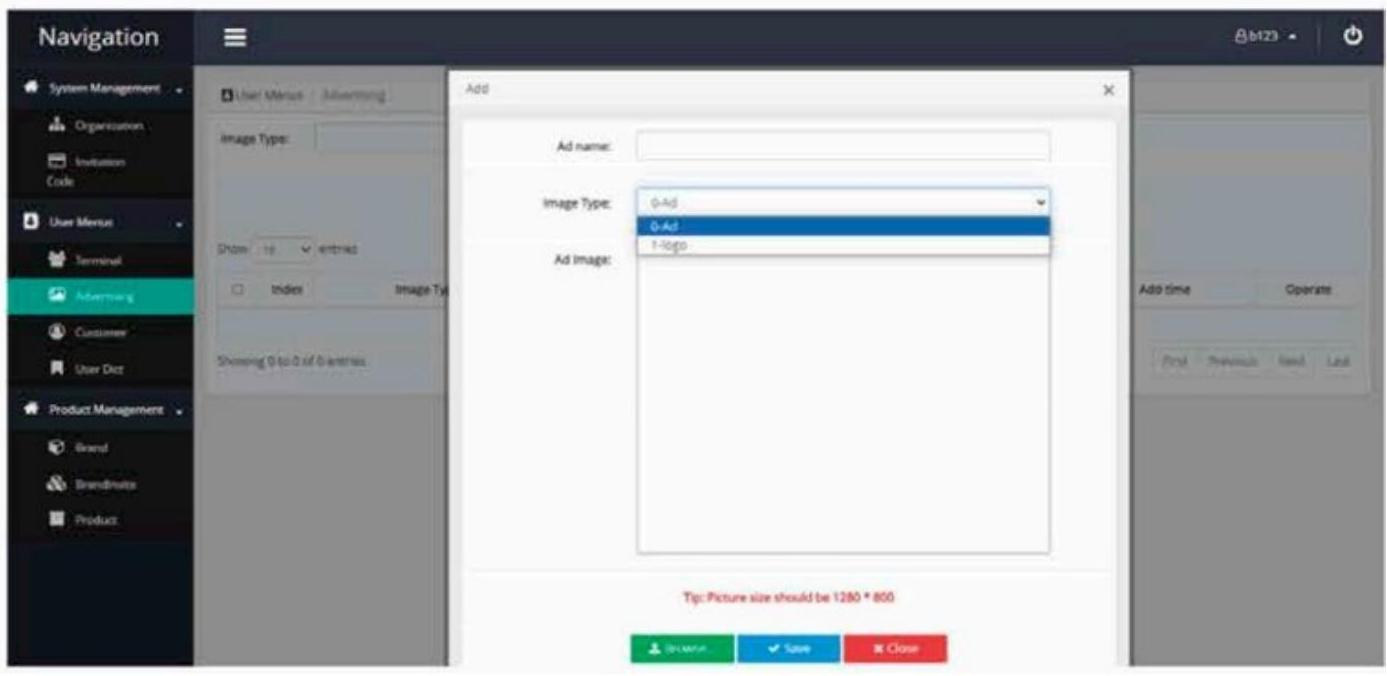
\includegraphics[alt={},max width=\textwidth]{018f02f8-3740-46eb-ab06-ecd68977d8ca-19_676_1387_1932_316}
\captionsetup{labelformat=empty}
\caption{Immagine 7-3-5}
\end{center}
\end{figure}

\subsubsection{Customer}
Nella parte inferiore del rapporto completo presente nel software di analisi, clicca su "Carica in cloud" per salvare il rapporto del client nel cloud. Successivamente, clicca sul "customer" nella nuvola per visualizzare il rapporto del cliente salvato \href{http://report.as}{report.as} come mostrato nella figura 7-3-6.\\
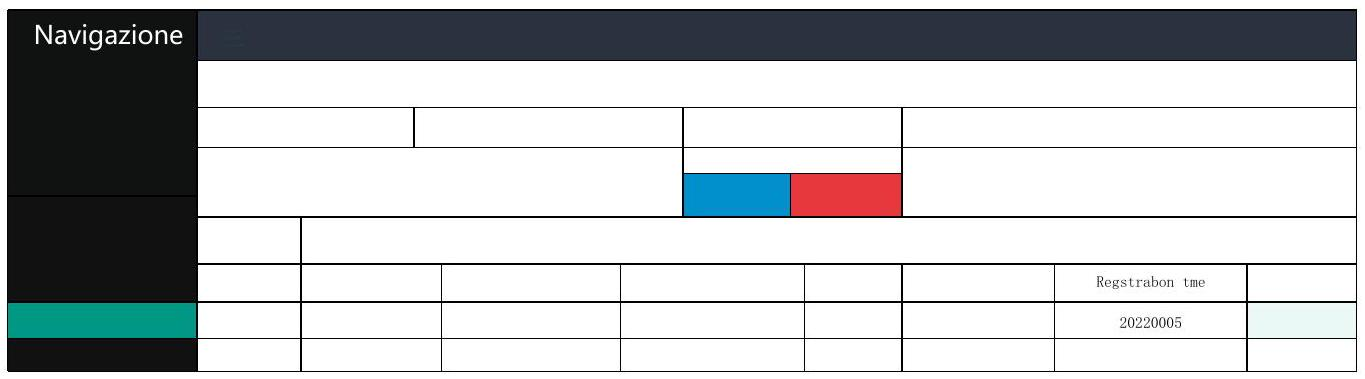
\includegraphics[max width=\textwidth, alt={}, center]{018f02f8-3740-46eb-ab06-ecd68977d8ca-19_379_1365_610_2423}

Clicca su "Dettagli"\\
visualizza il rapporto dettagliato del cliente, come mostrato nella figura 7-3-77-3-8.

\begin{center}
\begin{tabular}{|l|l|l|}
\hline
Navigazione & 三 & Bb \\
\hline
 &  &  \\
\hline
 &  &  \\
\hline
 & 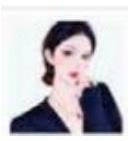
\includegraphics[max width=\textwidth, alt={}]{018f02f8-3740-46eb-ab06-ecd68977d8ca-19_141_133_1690_2992}
 &  \\
\hline
 &  &  \\
\hline
\end{tabular}
\end{center}

Immagine 7-3-7

\begin{figure}[H]
\begin{center}
  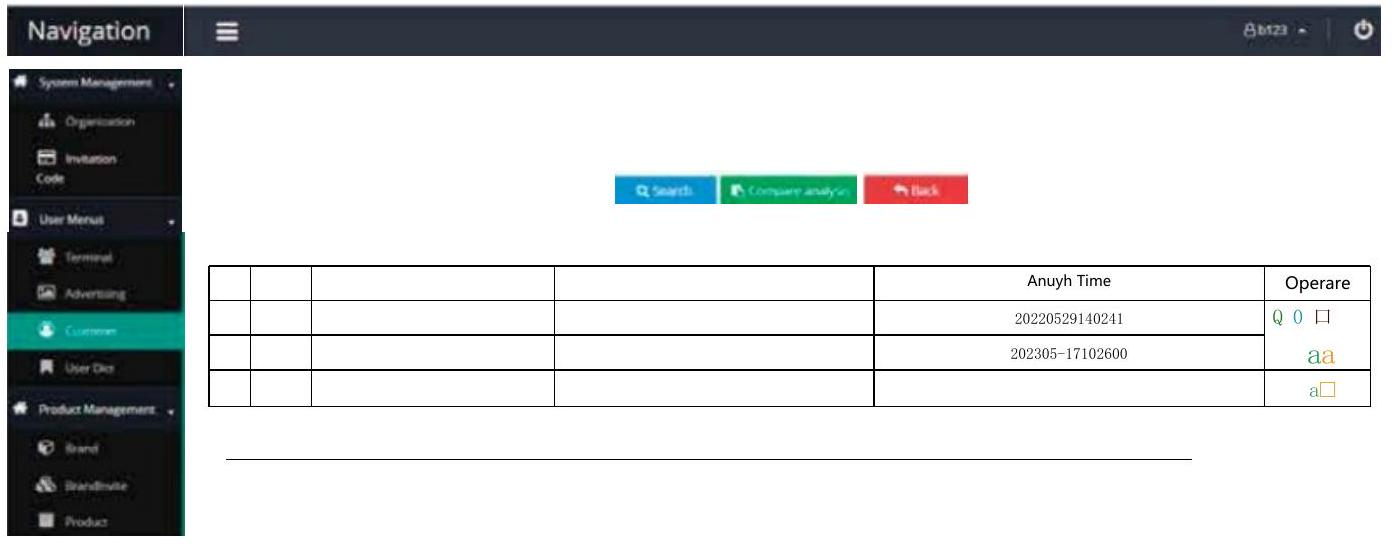
\includegraphics[alt={},max width=\textwidth]{018f02f8-3740-46eb-ab06-ecd68977d8ca-19_547_1394_2022_2423}
\captionsetup{labelformat=empty}
\caption{Immagine 7-3-8}
\end{center}
\end{figure}

Scegli due rapporti di analisi e fai clic su "Analisi comparativa" a consultare il rapporto di analisi comparativa, come illustrato nella figura 7-3-97-3-10.

\begin{figure}[H]
\begin{center}
  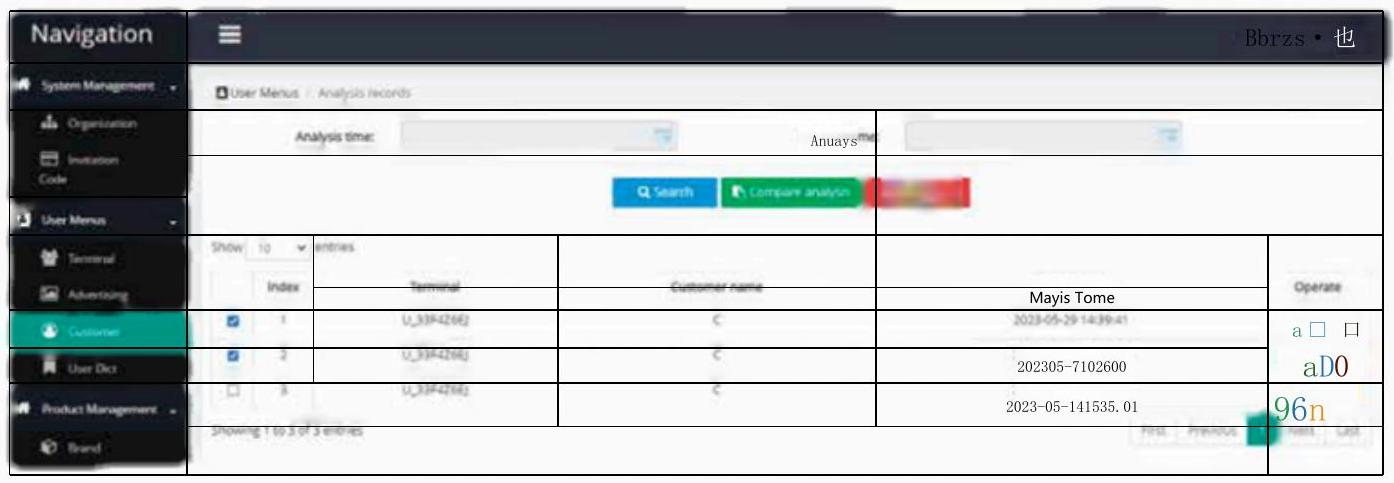
\includegraphics[alt={},max width=\textwidth]{018f02f8-3740-46eb-ab06-ecd68977d8ca-20_483_1394_529_355}
\captionsetup{labelformat=empty}
\caption{Picture7-3-9}
\end{center}
\end{figure}

\begin{figure}[H]
\begin{center}
  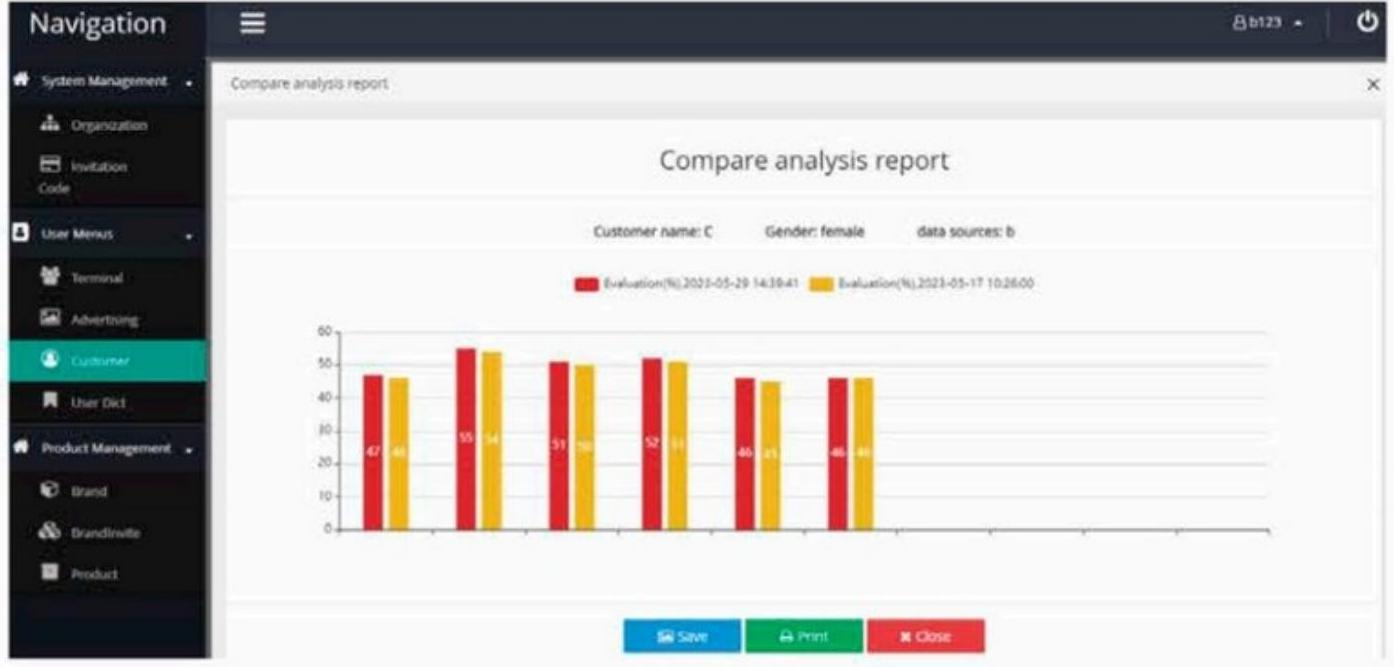
\includegraphics[alt={},max width=\textwidth]{018f02f8-3740-46eb-ab06-ecd68977d8ca-20_667_1394_1250_348}
\captionsetup{labelformat=empty}
\caption{Immagine 7-3-10}
\end{center}
\end{figure}

\section{Operare}
Fai clic su QDロ "Operate" per visualizzare il rapporto di analisi del cliente, il rapporto singolo e il rapporto completo, come mostrato nelle figure $7-3-11$, $7-3-12$ e $7-3-13$. Dopo aver collegato la stampante, fai clic su "Print" 母P s per stampare il rapporto cartaceo.\\
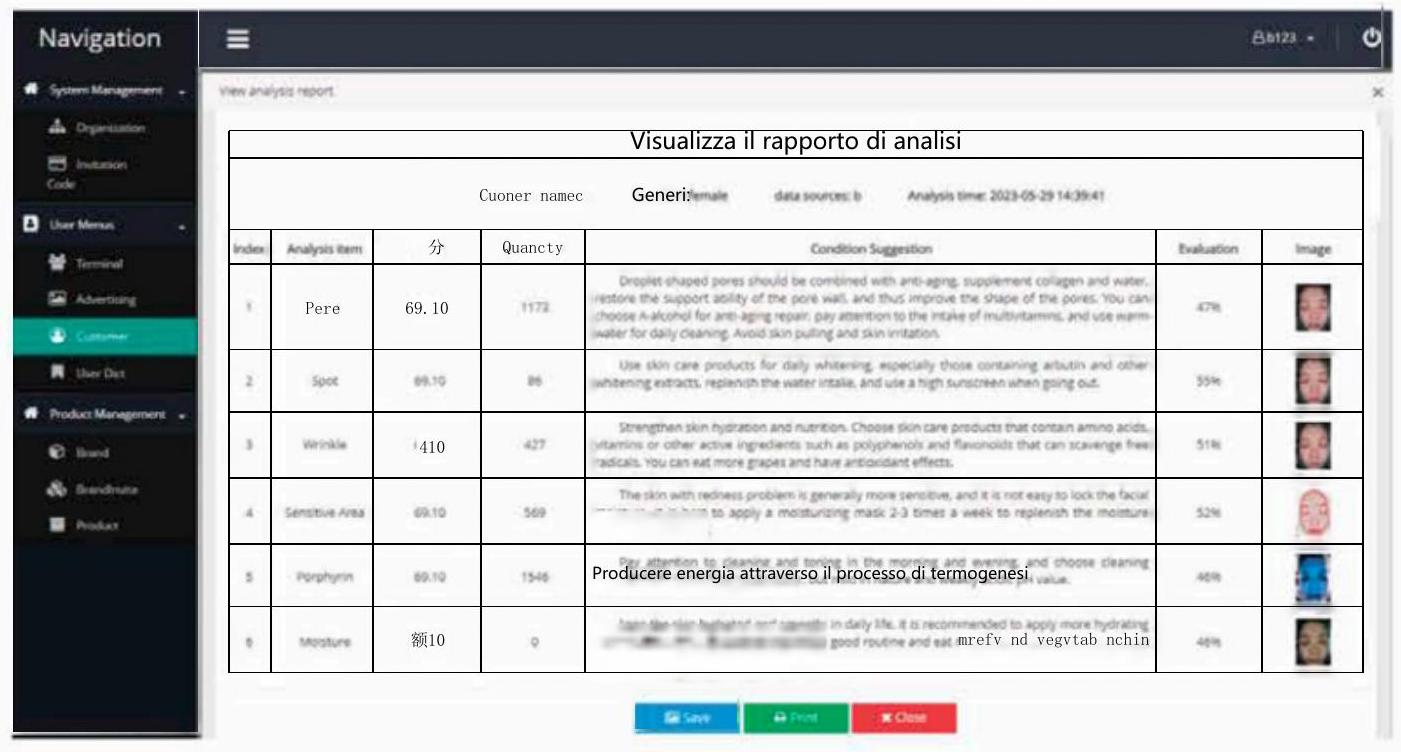
\includegraphics[max width=\textwidth, alt={}, center]{018f02f8-3740-46eb-ab06-ecd68977d8ca-20_752_1401_203_2434}

\begin{figure}[H]
\begin{center}
\captionsetup{labelformat=empty}
\caption{Immagine 7-3-11}
  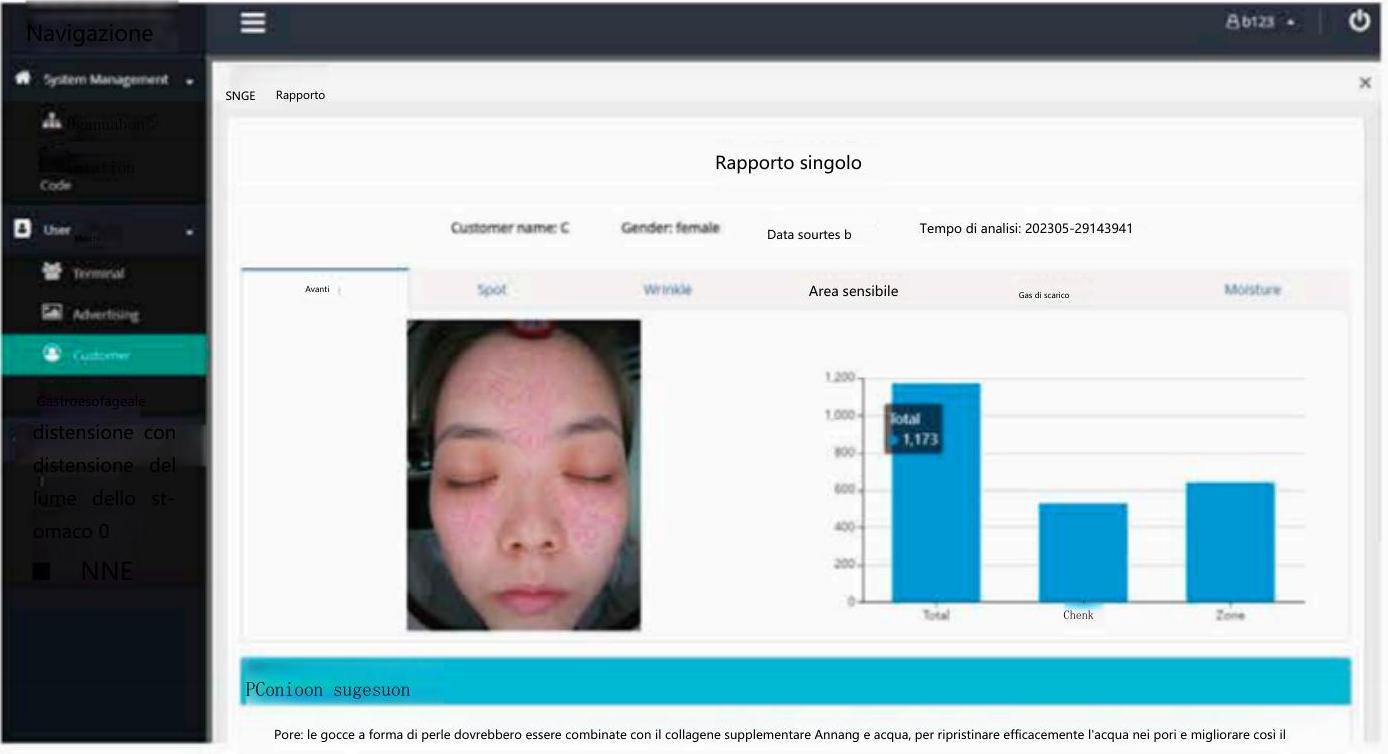
\includegraphics[alt={},max width=\textwidth]{018f02f8-3740-46eb-ab06-ecd68977d8ca-20_754_1388_1033_2429}
\end{center}
\end{figure}

\begin{figure}[H]
\begin{center}
\captionsetup{labelformat=empty}
\caption{Immagine 7-}
  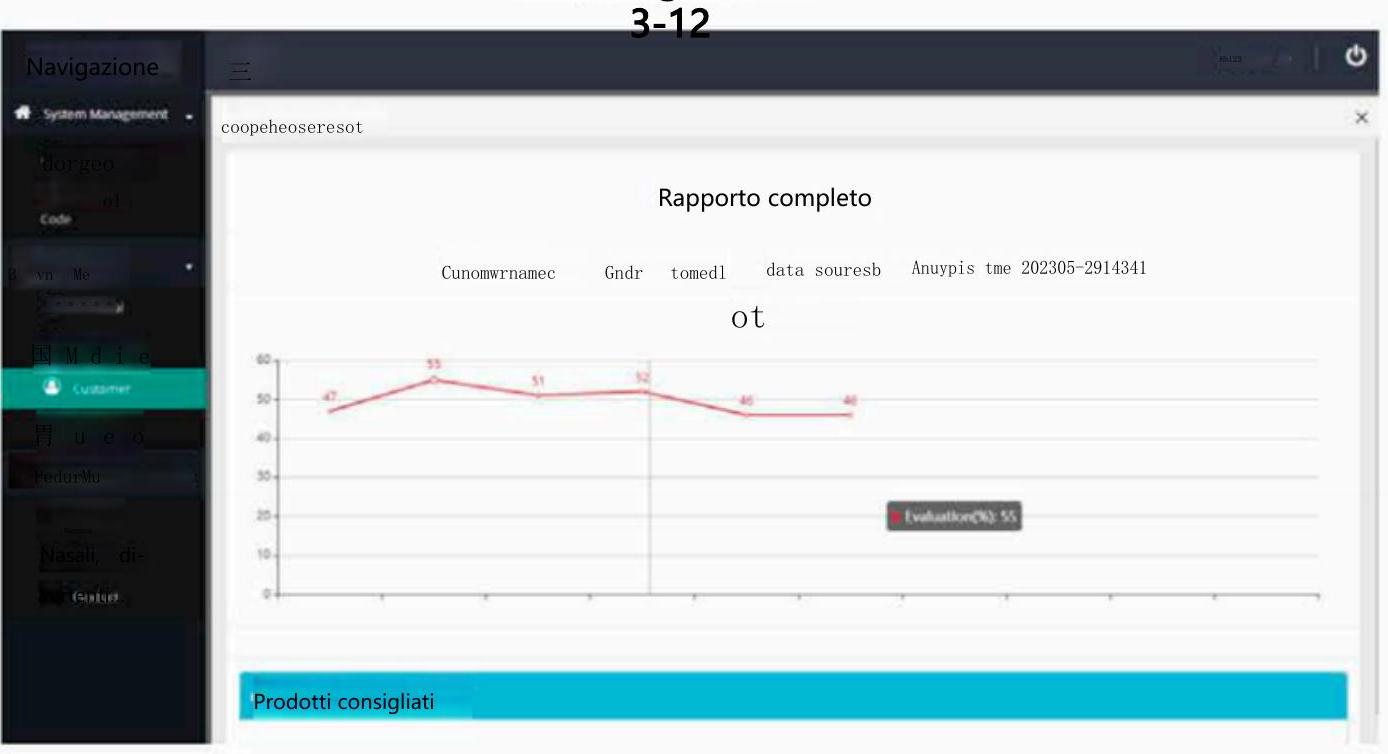
\includegraphics[alt={},max width=\textwidth]{018f02f8-3740-46eb-ab06-ecd68977d8ca-20_754_1388_1848_2429}
\end{center}
\end{figure}

Immagine 7-3-13

\subsubsection{Dizionario utente}
Fai clic su "User Dict" per modificare la "conditioning suggestion", come mostrato nella figura 7-3-14.\\
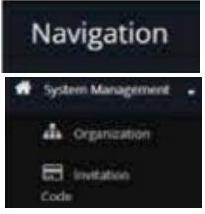
\includegraphics[max width=\textwidth, alt={}, center]{018f02f8-3740-46eb-ab06-ecd68977d8ca-21_214_205_546_361}\\
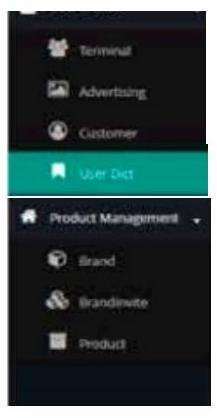
\includegraphics[max width=\textwidth, alt={}, center]{018f02f8-3740-46eb-ab06-ecd68977d8ca-21_418_217_781_355}

\begin{center}
\begin{tabular}{|l|l|l|l|l|l|l|l|l|}
\hline
 &  & n4y & Nome in codice & Codice della dieta & Detaut &  &  &  \\
\hline
 &  &  &  &  &  &  &  &  \\
\hline
 &  &  & Condtioning Sus8estion & FXM2 &  &  &  &  \\
\hline
 &  & N & ondnioning Suggesbon &  & Angolo &  &  &  \\
\hline
 &  &  & cohdmorung Susgestin &  &  &  &  &  \\
\hline
 &  & mL0t & Suggerimenti per la condizionamento & F0M5 &  &  &  &  \\
\hline
 &  & WL01 & Constoning sugeshon &  & Molsture &  &  &  \\
\hline
 &  & WL01 & condonazione di giustizia & PoMz &  & (omprehensvereport &  &  \\
\hline
\multicolumn{7}{|l|}{\begin{tabular}{l}
"howing 1t070f7entres" \\
Frt \\
\end{tabular}} &  &  \\
\hline
\end{tabular}
\end{center}

Immagine 7-3-14

Fai clic su "Modifica terminologia" cambiare la suggerizione di condizionamento, e questo\\
La sezione può essere modificata in base alle esigenze del tuo negozio, come mostrato nella figura 7-3-15.\\
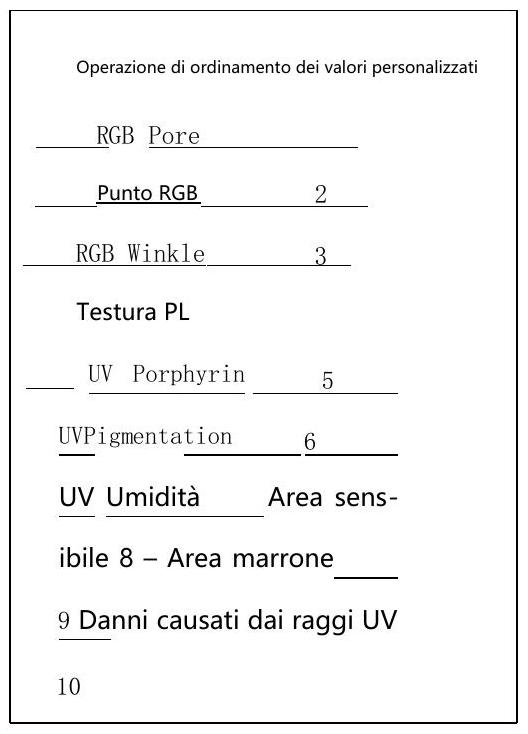
\includegraphics[max width=\textwidth, alt={}, center]{018f02f8-3740-46eb-ab06-ecd68977d8ca-21_734_528_1751_290}

\begin{figure}[H]
\begin{center}
  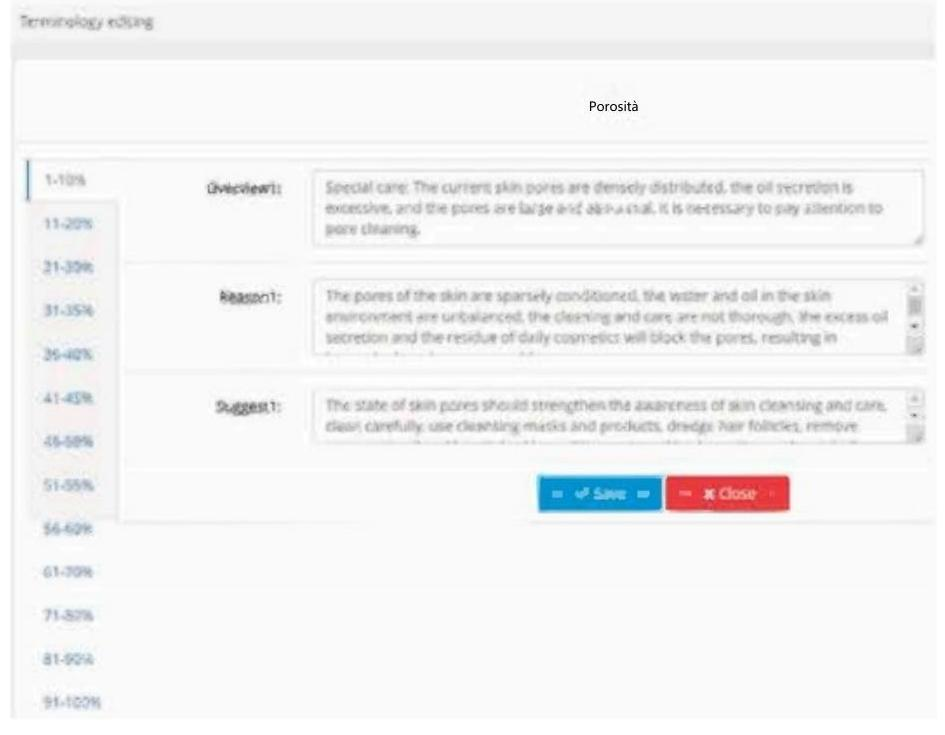
\includegraphics[alt={},max width=\textwidth]{018f02f8-3740-46eb-ab06-ecd68977d8ca-21_735_945_1757_833}
\captionsetup{labelformat=empty}
\caption{Immagine 7-3-15}
\end{center}
\end{figure}

\begin{figure}[H]
\begin{center}
\captionsetup{labelformat=empty}
\caption{Clicca cambiare il nome del progetto del prodotto, come mostrato nella figura 7-3-16.}
  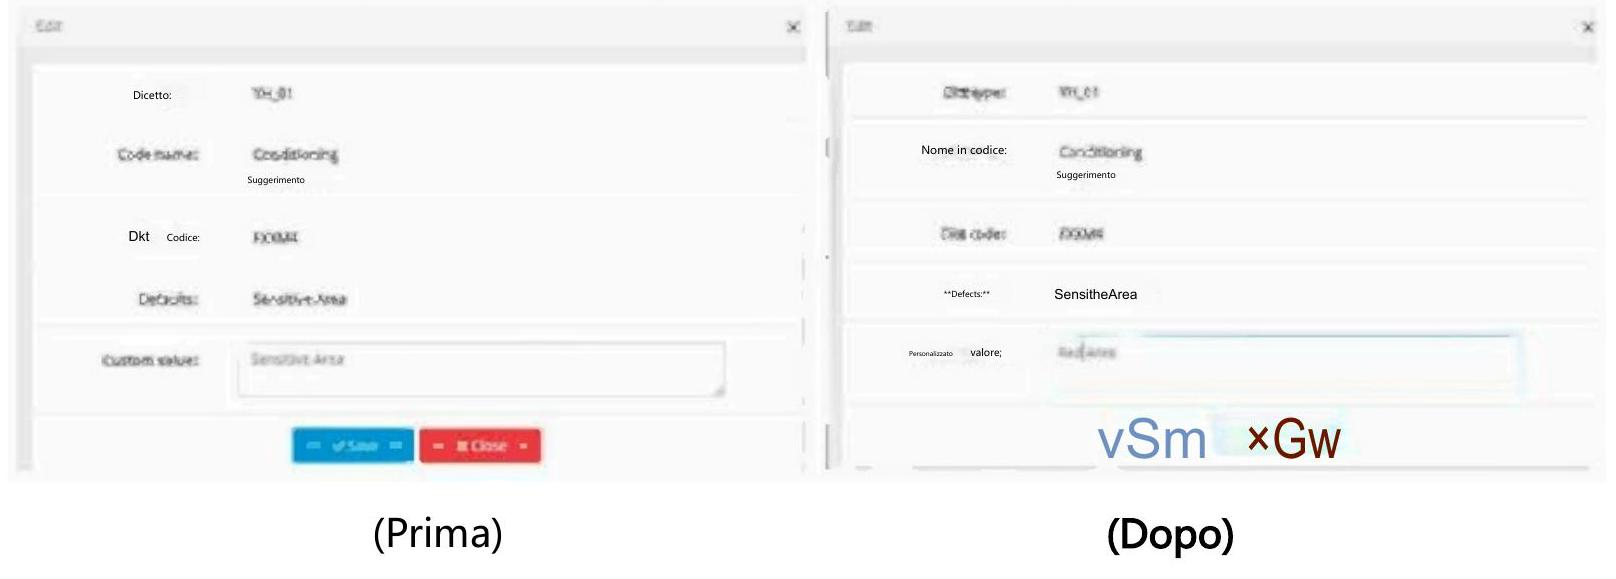
\includegraphics[alt={},max width=\textwidth]{018f02f8-3740-46eb-ab06-ecd68977d8ca-21_579_1616_420_2294}
\end{center}
\end{figure}

Immagine 7-3-16

\section{Elenco dei pacchi}
\begin{center}
\begin{tabular}{|l|l|l|l|}
\hline
Nome del prodotto & Quantità & Opzioni (V) & Nota \\
\hline
Corpo principale & 1 & ✓ &  \\
\hline
Manuale dell'utente & 1 & $\sqrt{ }$ &  \\
\hline
Certificato & 1 & ✓ &  \\
\hline
Carta di garanzia & 1 & ✓ &  \\
\hline
Linea elettrica & 1 & ✓ &  \\
\hline
Carta SD & 1 & ✓ &  \\
\hline
\end{tabular}
\end{center}

\section{Risoluzione dei problemi}
\begin{center}
\begin{tabular}{|l|l|l|l|}
\hline
No. & Sintomo & Motivo probabile & Metodo \\
\hline
1 & Il tablet non avvia. & \begin{tabular}{l}
A. La presa elettrica è lenta. \\
B. L'interruttore di alimentazione non è acceso. \\
C. L'ospite non è stato sottoposto a sputo \\
\end{tabular} & \begin{tabular}{l}
A. Si prega di collegare I' alimentazione. \\
B. Accendi l'alimentazione. \\
switch \\
C. Premi a lungo la tastiera principale per avviare il dispositivo \\
\end{tabular} \\
\hline
2 & Impossibile effettuare l'accesso al sistema. & Non ricordo il nome dell' account o la password & Contatta il produttore per richiedere la password. \\
\hline
3 & L'operazione di registrazione non è riuscita. & Il Wi-Fi non è connesso. & Connetti il Wi-Fi e registra di nuovo. \\
\hline
4 & Impossibile aggiornare il software & Il Wi-Fi non è connesso. & Chiudi il software, connetti il Wi-Fi e aggiorna di nuovo. \\
\hline
5 & "Shooting Crash" & Interferenza da parte di altri dispositivi estetici & Disattiva il dispositivo RF, Laser Interference. Riavvia il dispositivo. \\
\hline
\end{tabular}
\end{center}

\section{Manutenzione e riparazione}
\begin{enumerate}
  \item Utilizzare il dispositivo in modo corretto secondo le istruzioni del manuale d'uso e preservarne l'aspetto esterno durante l'uso.
  \item Non accendere il dispositivo in condizioni anomale.
  \item Durante l'uso, non controllare il dispositivo né modificare il modalità operativa con le mani bagnate.
  \item Dopo aver completato i test, verificate che il dispositivo sia normalmente chiuso, quindi pulite e controllate regolarmente il funzionamento del tecnico.
  \item Se il dispositivo presenta un difetto di qualità non umano entro una settimana dalla data di vendita, il fornitore è responsabile del rimborso, del rimpiazzo e della riparazione.
  \item Durante l'uso e la conservazione normali, se il prodotto presenta problemi di qualità entro il periodo di garanzia, si prega di contattare il fornitore per richiedere una risoluzione.
\end{enumerate}

Le seguenti condizioni non sono coperte dalla garanzia:\\
a. Il dispositivo è danneggiato o deformato a seguito di un impatto;\\
b. L'acqua entra nel dispositivo;\\
c. La rottura causata da smontaggio, riparazione e trasformazione;\\
d. Danni causati da un uso improprio;\\
e. Danni causati da calamità naturali impreviste (incendio, terremoto, alluvione, ecc.)

\section{Trasporto e Stoccaggio}
\begin{center}
\begin{tabular}{|l|l|}
\hline

\includegraphics[max width=\textwidth, alt={}]{018f02f8-3740-46eb-ab06-ecd68977d8ca-22_146_170_1802_2363}
 & \begin{tabular}{l}
Nota: \\
Questo dispositivo è adatto ai mezzi di trasporto comuni, come treni, automobili, navi e aerei. \\
\end{tabular} \\
\hline

\includegraphics[max width=\textwidth, alt={}]{018f02f8-3740-46eb-ab06-ecd68977d8ca-22_151_170_2023_2363}
 & \begin{tabular}{l}
Nota: \\
Durante il trasporto, il dispositivo deve essere protetto da vibrazioni, urti, cadute, sollevamenti e dalla pioggia. \\
\end{tabular} \\
\hline

\includegraphics[max width=\textwidth, alt={}]{018f02f8-3740-46eb-ab06-ecd68977d8ca-22_147_170_2253_2363}
 & \begin{tabular}{l}
Nota: \\
Il dispositivo deve essere conservato in un ambiente non corrosivo e ben ventilato. \\
\end{tabular} \\
\hline

\includegraphics[max width=\textwidth, alt={}]{018f02f8-3740-46eb-ab06-ecd68977d8ca-22_151_172_2483_2363}
 & \begin{tabular}{l}
Nota: \\
Quando il dispositivo non viene utilizzato per un lungo periodo, è consigliabile pulirlo conservarlo. Per evitare l'umidità, è meglio spegnere l'alimentazione una volta all'anno. \\
\end{tabular} \\
\hline
\end{tabular}
\end{center}

\section{Sperimenteri e Verifiche}
\begin{enumerate}
  \item Prima del sbarco, verificare l'imballaggio esterno per eventuali danni. In caso di danni, contattare il dipartimento competente e scattare delle foto. L'apertura della scatola è consentita esclusivamente con autorizzazione del dipartimento interessato. Se il dispositivo è danneggiato, la richiesta può essere inviata al dipartimento logistico.
  \item Dopo lo sbarco, verificare che l'elenco di imballaggio corrisponda alla merce effettiva (controllare l'elenco di imballaggio). In caso di mancanze, contattare immediatamente il reparto vendite dei dispositivi.
\end{enumerate}

\section{Protezione dell'ambiente}
Questo prodotto non influisce sull'ambiente dopo la sua smaltimento e non richiede alcun trattamento speciale. I clienti possono smontare il dispositivo e smaltirlo.

% --- INIZIO INFORMATIVA PRIVACY ---
\newpage

\section{INFORMATIVA PRIVACY}
\begin{center}
	(ai sensi dell'art. 13 del Regolamento UE 2016/679)
\end{center}

La presente informativa è resa ai sensi del Regolamento Generale sulla Protezione dei Dati (GDPR) e riguarda il trattamento dei dati personali dei clienti che si sottopongono a trattamenti e tecnologie estetiche.

\subsection*{Titolare del trattamento}

Il Titolare del trattamento è:

\begin{itemize}
	\item Denominazione centro estetico: \underline{\hspace{5cm}}
	\item Sede legale: \underline{\hspace{7cm}}
	\item P. IVA / C.F.: \underline{\hspace{6cm}}
	\item Contatti (telefono/email): \underline{\hspace{5cm}}
\end{itemize}

\subsection*{Tipologia di dati trattati}

Il Titolare può raccogliere e trattare le seguenti categorie di dati:

\begin{itemize}
	\item Dati anagrafici (nome, cognome, data di nascita)
	\item Dati di contatto (telefono, e-mail)
	\item Dati fiscali per eventuale fatturazione
	\item Dati particolari relativi allo stato di salute (allergie, patologie, gravidanza, terapie in corso) necessari per valutare l'idoneità ai trattamenti estetici
	\item Eventuali immagini fotografiche prima/dopo trattamento (previo consenso specifico)
\end{itemize}

\subsection*{Finalità del trattamento}

I dati personali sono trattati per le seguenti finalità:

\begin{enumerate}
	\item Esecuzione di trattamenti estetici e utilizzo di tecnologie professionali (laser, radiofrequenza, ultrasuoni, pressoterapia, ecc.)
	\item Valutazione dell'idoneità al trattamento
	\item Adempimenti amministrativi, contabili e fiscali
	\item Gestione degli appuntamenti
	\item Eventuale invio di comunicazioni promozionali (solo previo consenso separato)
	\item Eventuale utilizzo di immagini per finalità informative o promozionali (solo previo consenso separato)
\end{enumerate}

\subsection*{Base giuridica del trattamento}

Il trattamento dei dati si fonda su:

\begin{itemize}
	\item Esecuzione del contratto/prestazione richiesta
	\item Adempimento di obblighi di legge
	\item Consenso esplicito dell'interessato per il trattamento di dati particolari (sanitari)
	\item Consenso separato per marketing e utilizzo immagini
\end{itemize}

\subsection*{Modalità di trattamento}

Il trattamento dei dati avviene mediante strumenti cartacei e/o informatici, nel rispetto dei principi di correttezza, liceità, trasparenza e tutela della riservatezza.

Sono adottate adeguate misure di sicurezza per prevenire accessi non autorizzati, perdita o diffusione dei dati.

\subsection*{Conservazione dei dati}

I dati personali saranno conservati:

\begin{itemize}
	\item Per il tempo necessario all'erogazione del servizio
	\item Per il periodo previsto dalla normativa fiscale e civilistica
	\item Fino a revoca del consenso per finalità di marketing o utilizzo immagini
\end{itemize}

\subsection*{Comunicazione dei dati}

I dati potranno essere comunicati a:

\begin{itemize}
	\item Consulenti fiscali e amministrativi
	\item Software gestionali utilizzati per la gestione clienti
	\item Autorità competenti, ove previsto dalla legge
\end{itemize}

I dati non saranno diffusi senza consenso.

\subsection*{Diritti dell'interessato}

L'interessato può esercitare in qualsiasi momento i seguenti diritti:

\begin{itemize}
	\item Accesso ai propri dati
	\item Rettifica o aggiornamento
	\item Cancellazione (diritto all'oblio)
	\item Limitazione del trattamento
	\item Opposizione al trattamento
	\item Revoca del consenso
	\item Reclamo all'Autorità Garante per la Protezione dei Dati Personali
\end{itemize}

Le richieste possono essere inviate ai recapiti del Titolare sopra indicati.

\subsection*{Natura del conferimento dei dati}

Il conferimento dei dati è necessario per l'erogazione dei trattamenti estetici.
Il mancato conferimento può comportare l'impossibilità di eseguire il servizio.

\subsection*{CONSENSO}

Il/La sottoscritto/a dichiara di aver ricevuto e compreso la presente informativa.

\vspace{0.8cm}

Data: \underline{\hspace{5cm}} 

\vspace{15pt}
Firma: \underline{\hspace{6cm}}

\vspace{1cm}

$\square$ Acconsento al trattamento dei dati particolari (sanitari)

\vspace{0.3cm}
$\square$ Acconsento all'utilizzo delle immagini per finalità promozionali

\vspace{0.3cm}
$\square$ Acconsento a ricevere comunicazioni promozionali

% --- FINE INFORMATIVA PRIVACY ---

\newpage


\begin{figure}[H]
	\centering
	\includegraphics[width=0.7\paperwidth,height=\paperheight, keepaspectratio]{"../cose da aggiungere/privacy_conformita/dichiarazione_conformita"}
\end{figure}


\end{document}